% This is the main LaTeX file which is used to produce the Biopython
% Tutorial documentation.
%
% If you just want to read the documentation, you can pick up ready-to-go
% copies in both pdf and html format from:
%
% http://biopython.org/DIST/docs/tutorial/Tutorial.html
% http://biopython.org/DIST/docs/tutorial/Tutorial.pdf
%
% If you want to typeset the documentation, you'll need a standard TeX/LaTeX
% distribution (I use teTeX, which works great for me on unix platforms).
% Additionally, you need HeVeA (or at least hevea.sty), which can be
% found at:
%
% http://pauillac.inria.fr/~maranget/hevea/index.html
%

% You will also need the pictures included in the document, which are
% UMLish diagrams created by Dia
% (http://www.lysator.liu.se/~alla/dia/dia.html).
% These diagrams are available from biopython CVS in the original dia
% format, which you can easily save as .png format using Dia itself.
% They are also checked in as the png files, so if you make
% modifications to the original dia files, the png files should also be
% changed.
%
% Once you're all set, you should be able to generate pdf by running:
%

% pdflatex Tutorial.tex  (to generate the first draft)
% pdflatex Tutorial.tex  (to get the cross references right)
% pdflatex Tutorial.tex  (to get the table of contents right)
%
% To generate the html, you'll need HeVeA installed. First, remove the
% Tutorial.aux file generated by LaTeX, then run:
%

% hevea -fix Tutorial.tex   (to generate the html file)
% hevea -fix Tutorial.tex   (to get the references correct)
% hacha Tutorial.html  (to split the html file into sections)
%
% If you want to typeset this and have problems, please report them
% at biopython-dev@biopython.org, and we'll try to get things resolved. We
% always love to have people interested in the documentation!

\documentclass{report}
\usepackage{url}
\usepackage{fullpage}
\usepackage{hevea}
\usepackage{graphicx}

% make everything have section numbers
\setcounter{secnumdepth}{4}

% Make links between references
\usepackage{hyperref}
\newif\ifpdf
\ifx\pdfoutput\undefined
  \pdffalse
\else
  \pdfoutput=1
  \pdftrue
\fi
\ifpdf
  \hypersetup{colorlinks=true, hyperindex=true, citecolor=red, urlcolor=blue}
\fi

\begin{document}

\title{Biopython Tutorial and Cookbook}
\author{Jeff Chang, Brad Chapman, Iddo Friedberg, Thomas Hamelryck, Michiel de Hoon, Peter Cock}
\date{Last Update -- September 2008}

\maketitle
\tableofcontents

\chapter{Introduction}
\label{chapter:introduction}

\section{What is Biopython?}

The Biopython Project is an international association of developers of freely available Python (\url{http://www.python.org}) tools for computational molecular biology. The web site \url{http://www.biopython.org} provides an online resource for modules, scripts, and web links for developers of Python-based software for life science research.

Basically, we just like to program in python and want to make it as easy as possible to use python for bioinformatics by creating high-quality, reusable modules and scripts.

\subsection{What can I find in the Biopython package}

The main Biopython releases have lots of functionality, including:

\begin{itemize}
  \item The ability to parse bioinformatics files into python utilizable data structures, including support for the following formats:

  \begin{itemize}
    \item Blast output -- both from standalone and WWW Blast
    \item Clustalw
    \item FASTA
    \item GenBank
    \item PubMed and Medline
    \item ExPASy files, like Enzyme, Prodoc and Prosite
    \item SCOP, including `dom' and `lin' files
    \item UniGene
    \item SwissProt
  \end{itemize}

  \item Files in the supported formats can be iterated over record by record or indexed and accessed via a Dictionary interface.

  \item Code to deal with popular on-line bioinformatics destinations such as:

  \begin{itemize}
    \item NCBI -- Blast, Entrez and PubMed services
    \item ExPASy -- Prodoc and Prosite entries
  \end{itemize}

  \item Interfaces to common bioinformatics programs such as:

  \begin{itemize}
    \item Standalone Blast from NCBI
    \item Clustalw alignment program.
  \end{itemize}

  \item A standard sequence class that deals with sequences, ids on sequences, and sequence features.

  \item Tools for performing common operations on sequences, such as translation, transcription and weight calculations.

  \item Code to perform classification of data using k Nearest Neighbors, Naive Bayes or Support Vector Machines.

  \item Code for dealing with alignments, including a standard way to create and deal with substitution matrices.

  \item Code making it easy to split up parallelizable tasks into separate processes.

  \item GUI-based programs to do basic sequence manipulations, translations, BLASTing, etc.

  \item Extensive documentation and help with using the modules, including this file, on-line wiki documentation, the web site, and the mailing list.

  \item Integration with BioSQL, a sequence database schema also supported by the BioPerl and BioJava projects.

\end{itemize}

We hope this gives you plenty of reasons to download and start using Biopython!

\section{Installing Biopython}

All of the installation information for Biopython was separated from
this document to make it easier to keep updated.

The short version is go to our downloads page (\url{http://biopython.org/wiki/Download}),
download and install the listed dependencies, then download and install Biopython.
For Windows we provide pre-compiled click-and-run installers, while for Unix and other
operating systems you must install from source as described in the included README file.
This is usually as simple as the standard command:

\begin{verbatim}
sudo python setup.py install
\end{verbatim}

The longer version of our installation instructions covers
installation of python, Biopython dependencies and Biopython itself.
It is available in PDF
(\url{http://biopython.org/DIST/docs/install/Installation.pdf})
and HTML formats
(\url{http://biopython.org/DIST/docs/install/Installation.html}).

\section{FAQ}

\begin{enumerate}

  \item \emph{Why doesn't} \verb|Bio.SeqIO| \emph{work? It imports fine but there is no parse function etc.} \\
  You need Biopython 1.43 or later.  Older versions did contain some related code under the \verb|Bio.SeqIO| name which has since been deprecated - and this is why the import ``works''.

  \item \emph{Why doesn't} \verb|Bio.SeqIO.read()| \emph{work? The module imports fine but there is no read function!} \\
  You need Biopython 1.45 or later.

  \item \emph{What file formats do} \verb|Bio.SeqIO| \emph{and} \verb|Bio.AlignIO| \emph{read and write?} \\
  See \url{http://biopython.org/wiki/SeqIO} and \url{http://biopython.org/wiki/AlignIO} on the wiki for the latest listing.
  
  \item \emph{Why doesn't} \verb|str(...)| \emph{give me the full sequence of a} \verb|Seq| \emph{object?} \\
  You need Biopython 1.45 or later.  Alternatively, rather than \verb|str(my_seq)|, use \verb|my_seq.tostring()| (which will also work on recent versions of Biopython).
  
  \item \emph{Why doesn't} \verb|Bio.Blast| \emph{work with the latest plain text NCBI blast output?} \\
  The NCBI keep tweaking the plain text output from the BLAST tools, and keeping our parser up to date is an ongoing struggle.  We recommend you use the XML output instead, which is designed to be read by a computer program.

  \item \emph{Why isn't} \verb|Bio.AlignIO| \emph{present? The module import fails!} \\
  You need Biopython 1.46 or later.

  \item \emph{Why doesn't} \verb|Bio.Entrez.read()| \emph{work? The module imports fine but there is no read function!} \\
  You need Biopython 1.46 or later.

  \item \emph{I looked in a directory for code, but I couldn't seem to find the code that does something. Where's it hidden?} \\
  One thing to know is that we put code in \verb|__init__.py| files. If you are not used to looking for code in this file this can be confusing. The reason we do this is to make the imports easier for users. For instance, instead of having to do a ``repetitive'' import like \verb|from Bio.GenBank import GenBank|, you can just use \verb|from Bio import GenBank|.

\end{enumerate}

\chapter{Quick Start -- What can you do with Biopython?}
\label{chapter:quick-start}

This section is designed to get you started quickly with Biopython, and to give a general overview of what is available and how to use it. All of the examples in this section assume that you have some general working knowledge of python, and that you have successfully installed Biopython on your system. If you think you need to brush up on your python, the main python web site provides quite a bit of free documentation to get started with (\url{http://www.python.org/doc/}).

Since much biological work on the computer involves connecting with databases on the internet, some of the examples will also require a working internet connection in order to run.

Now that that is all out of the way, let's get into what we can do with Biopython.

\section{General overview of what Biopython provides}

As mentioned in the introduction, Biopython is a set of libraries to provide the ability to deal with ``things'' of interest to biologists working on the computer. In general this means that you will need to have at least some programming experience (in python, of course!) or at least an interest in learning to program. Biopython's job is to make your job easier as a programmer by supplying reusable libraries so that you can focus on answering your specific question of interest, instead of focusing on the internals of parsing a particular file format (of course, if you want to help by writing a parser that doesn't exist and contributing it to Biopython, please go ahead!). So Biopython's job is to make you happy!

One thing to note about Biopython is that it often provides multiple ways of ``doing the same thing.'' Things have improved in recent releases, but this can still be frustrating to me since I often way to just know the one right way to do something. However, this is also a real benefit because it gives you lots of flexibility and control over the libraries. The tutorial helps to show you the common or easy ways to do things so that you can just make things work. To learn more about the alternative possibilities, look into the Cookbook (Chapter~\ref{chapter:cookbook}, this has some cools tricks and tips) and the Advanced section (which provides you with as much detail as you'd ever want to know!).

\section{Working with sequences}
\label{sec:sequences}

Disputably (of course!), the central object in bioinformatics is the sequence. Thus, we'll start with a quick introduction to the Biopython mechanisms for dealing with sequences, the \verb|Seq| object, which we'll discuss in more detail in Chapter~\ref{chapter:Bio.Seq}.

Most of the time when we think about sequences we have in my mind a string of letters like \verb|'AGTACACTGGT'|. You can create such \verb|Seq| object with this sequence as follows - the ``$>>>$'' represents the python prompt followed by what you would type in:

\begin{verbatim}
>>> from Bio.Seq import Seq
>>> my_seq = Seq("AGTACACTGGT")
>>> my_seq
Seq('AGTACACTGGT', Alphabet())
>>> print my_seq
AGTACACTGGT
>>> my_seq.alphabet
Alphabet()
\end{verbatim}

What we have here is a sequence object with a \emph{generic} alphabet - reflecting the fact we have \emph{not} specified if this is a DNA or protein sequence (okay, a protein with a lot of Alanines, Glycines, Cysteines and Threonines!).  We'll talk more about alphabets in Chapter~\ref{chapter:Bio.Seq}.

In addition to having an alphabet, the \verb|Seq| object differs from the python string in the methods it supports.  You can't do this with a plain string:

\begin{verbatim}
>>> my_seq
Seq('AGTACACTGGT', Alphabet())
>>> my_seq.complement()
Seq('TCATGTGACCA', Alphabet())
>>> my_seq.reverse_complement()
Seq('ACCAGTGTACT', Alphabet())
\end{verbatim}

The next most important class is the \verb|SeqRecord| or Sequence Record.  This holds a sequence (as a \verb|Seq| object) with additional annotation including an identifier, name and description.  The \verb|Bio.SeqIO| module for reading and writing sequence file formats works with \verb|SeqRecord| objects, which will be introduced below and covered in more detail by Chapter~\ref{chapter:Bio.SeqIO}.

This covers the basic features and uses of the Biopython sequence class.
Now that you've got some idea of what it is like to interact with the Biopython libraries, it's time to delve into the fun, fun world of dealing with biological file formats!

\section{A usage example}
\label{sec:orchids}

Before we jump right into parsers and everything else to do with Biopython, let's set up an example to motivate everything we do and make life more interesting. After all, if there wasn't any biology in this tutorial, why would you want you read it?

Since I love plants, I think we're just going to have to have a plant based example (sorry to all the fans of other organisms out there!).  Having just completed a recent trip to our local greenhouse, we've suddenly developed an incredible obsession with Lady Slipper Orchids (if you wonder why, have a look at some \href{http://www.flickr.com/search/?q=lady+slipper+orchid&s=int&z=t}{Lady Slipper Orchids photos on Flickr}, or try a \href{http://images.google.com/images?q=lady%20slipper%20orchid}{Google Image Search}).

Of course, orchids are not only beautiful to look at, they are also extremely interesting for people studying evolution and systematics. So let's suppose we're thinking about writing a funding proposal to do a molecular study of Lady Slipper evolution, and would like to see what kind of research has already been done and how we can add to that.

% Brad's links to Millicent Orchids are dead now (March 2007)
% http://www.millicentorchids.com/greenhouse/images/papesq01.jpg
% http://www.millicentorchids.com/greenhouse/indexphoto.htm

After a little bit of reading up we discover that the Lady Slipper Orchids are in the Orchidaceae family and the Cypripedioideae sub-family and are made up of 5 genera:  \emph{Cypripedium}, \emph{Paphiopedilum}, \emph{Phragmipedium}, \emph{Selenipedium} and \emph{Mexipedium}.

That gives us enough to get started delving for more information. So, let's look at how the Biopython tools can help us.  We'll start with sequence parsing in Section~\ref{sec:sequence-parsing}, but the orchids will be back later on as well - for example we'll search PubMed for papers about orchids and extract sequence data from GenBank in Chapter~\ref{chapter:entrez}, extract data from Swiss-Prot from certain orchid proteins in Chapter~\ref{chapter:swiss_prot}, and work with ClustalW multiple sequence alignments of orchid proteins in Section~\ref{sec:align_clustal}.

\section{Parsing sequence file formats}
\label{sec:sequence-parsing}

A large part of much bioinformatics work involves dealing with the many types of file formats designed to hold biological data. These files are loaded with interesting biological data, and a special challenge is parsing these files into a format so that you can manipulate them with some kind of programming language. However the task of parsing these files can be frustrated by the fact that the formats can change quite regularly, and that formats may contain small subtleties which can break even the most well designed parsers.

We are now going to briefly introduce the \verb|Bio.SeqIO| module -- you can find out more in Chapter~\ref{chapter:Bio.SeqIO}.  We'll start with an online search for our friends, the lady slipper orchids. To keep this introduction simple, we're just using the NCBI website by hand.  Let's just take a look through the nucleotide databases at NCBI, using an Entrez online search (\url{http://www.ncbi.nlm.nih.gov:80/entrez/query.fcgi?db=Nucleotide}) for everything mentioning the text Cypripedioideae (this is the subfamily of lady slipper orchids).  

When this tutorial was originally written, this search gave us only 94 hits, which we saved as a FASTA formatted text file and as a GenBank formatted text file (files \href{http://biopython.org/DIST/docs/tutorial/examples/ls_orchid.fasta}{\tt ls\_orchid.fasta} and \href{http://biopython.org/DIST/docs/tutorial/examples/ls_orchid.gbk}{\tt ls\_orchid.gbk}, also included with the Biopython source code under {\tt docs/tutorial/examples/}).

% The GenBank version is actually new - it was created by filtering out the original 94 hits from the
% latest search of over 400 hits.

If you run the search today, you'll get hundreds of results!  When following the tutorial, if you want to see the same list of genes, just download the two files above or copy them from \verb|docs/examples/| in the Biopython source code.  In Section~\ref{sec:connecting-with-biological-databases} we will look at how to do a search like this from within python.

\subsection{Simple FASTA parsing example}
\label{sec:fasta-parsing}

If you open the lady slipper orchids FASTA file \href{http://biopython.org/DIST/docs/tutorial/examples/ls_orchid.fasta}{\tt ls\_orchid.fasta} in your favourite text editor, you'll see that the file starts like this:

\begin{verbatim}
>gi|2765658|emb|Z78533.1|CIZ78533 C.irapeanum 5.8S rRNA gene and ITS1 and ITS2 DNA
CGTAACAAGGTTTCCGTAGGTGAACCTGCGGAAGGATCATTGATGAGACCGTGGAATAAACGATCGAGTG
AATCCGGAGGACCGGTGTACTCAGCTCACCGGGGGCATTGCTCCCGTGGTGACCCTGATTTGTTGTTGGG
...
\end{verbatim}

It contains 94 records, each has a line starting with ``$>$'' (greater-than symbol) followed by the sequence on one or more lines.  Now try this in python:

\begin{verbatim}
from Bio import SeqIO
handle = open("ls_orchid.fasta")
for seq_record in SeqIO.parse(handle, "fasta") :
    print seq_record.id
    print repr(seq_record.seq)
    print len(seq_record)
handle.close()
\end{verbatim}

\noindent You should get something like this on your screen:

\begin{verbatim}
gi|2765658|emb|Z78533.1|CIZ78533
Seq('CGTAACAAGGTTTCCGTAGGTGAACCTGCGGAAGGATCATTGATGAGACCGTGG...CGC', SingleLetterAlphabet())
740
...
gi|2765564|emb|Z78439.1|PBZ78439
Seq('CATTGTTGAGATCACATAATAATTGATCGAGTTAATCTGGAGGATCTGTTTACT...GCC', SingleLetterAlphabet())
592
\end{verbatim}

Notice that the FASTA format does not specify the alphabet, so \verb|Bio.SeqIO| has defaulted to the rather generic \verb|SingleLetterAlphabet()| rather than something DNA specific.

\subsection{Simple GenBank parsing example}

Now let's load the GenBank file \href{http://biopython.org/DIST/docs/tutorial/examples/ls_orchid.gbk}{\tt ls\_orchid.gbk} instead - notice that the code to do this is almost identical to the snippet used above for the FASTA file - the only difference is we change the filename and the format string:

\begin{verbatim}
from Bio import SeqIO
handle = open("ls_orchid.gbk")
for seq_record in SeqIO.parse(handle, "genbank") :
    print seq_record.id
    print repr(seq_record.seq)
    print len(seq_record)
handle.close()
\end{verbatim}

\noindent This should give:

\begin{verbatim}
Z78533.1
Seq('CGTAACAAGGTTTCCGTAGGTGAACCTGCGGAAGGATCATTGATGAGACCGTGG...CGC', IUPACAmbiguousDNA())
740
...
Z78439.1
Seq('CATTGTTGAGATCACATAATAATTGATCGAGTTAATCTGGAGGATCTGTTTACT...GCC', IUPACAmbiguousDNA())
592
\end{verbatim}

This time \verb|Bio.SeqIO| has been able to choose a sensible alphabet, IUPAC Ambiguous DNA.  You'll also notice that a shorter string has been used as the \verb|seq_record.id| in this case.

\subsection{I love parsing -- please don't stop talking about it!}

Biopython has a lot of parsers, and each has its own little special niches based on the sequence format it is parsing and all of that.  Chapter~\ref{chapter:Bio.SeqIO} covers \verb|Bio.SeqIO| in more detail, while Chapter~\ref{chapter:Bio.AlignIO} introduces \verb|Bio.AlignIO| for sequence alignments.

While the most popular file formats have parsers integrated into \verb|Bio.SeqIO| and/or \verb|Bio.AlignIO|, for some of the rarer and unloved file formats there is either no parser at all, or an old parser which has not been linked in yet.
Please also check the wiki pages \url{http://biopython.org/wiki/SeqIO} and \url{http://biopython.org/wiki/AlignIO} for the latest information, or ask on the mailing list. The wiki pages should include an up to date list of supported file types, and some additional  examples.

The next place to look for information about specific parsers and how to do cool things with them is in the Cookbook (Chapter~\ref{chapter:cookbook} of this Tutorial). If you don't find the information you are looking for, please consider helping out your poor overworked documentors and submitting a cookbook entry about it! (once you figure out how to do it, that is!)

\section{Connecting with biological databases}
\label{sec:connecting-with-biological-databases}

One of the very common things that you need to do in bioinformatics is extract information from biological databases. It can be quite tedious to access these databases manually, especially if you have a lot of repetitive work to do. Biopython attempts to save you time and energy by making some on-line databases available from python scripts. Currently, Biopython has code to extract information from the following databases:

\begin{itemize}
  \item \href{http://www.ncbi.nlm.nih.gov/Entrez/}{Entrez} (and \href{http://www.ncbi.nlm.nih.gov/PubMed/}{PubMed}) from the NCBI -- See Chapter~\ref{chapter:entrez}.
  \item \href{http://www.expasy.org/}{ExPASy} -- See Chapter~\ref{chapter:swiss_prot}.
  \item \href{http://scop.mrc-lmb.cam.ac.uk/scop/}{SCOP} -- See the \verb|Bio.SCOP.search()| function.
\end{itemize}

The code in these modules basically makes it easy to write python code that interact with the CGI scripts on these pages, so that you can get results in an easy to deal with format. In some cases, the results can be tightly integrated with the Biopython parsers to make it even easier to extract information.

\section{What to do next}

Now that you've made it this far, you hopefully have a good understanding of the basics of Biopython and are ready to start using it for doing useful work. The best thing to do now is finish reading this tutorial, and then if you want start snooping around in the source code, and looking at the automatically generated documentation.

Once you get a picture of what you want to do, and what libraries in Biopython will do it, you should take a peak at the Cookbook (Chapter~\ref{chapter:cookbook}), which may have example code to do something similar to what you want to do.

If you know what you want to do, but can't figure out how to do it, please feel free to post questions to the main biopython list (see \url{http://biopython.org/wiki/Mailing_lists}). This will not only help us answer your question, it will also allow us to improve the documentation so it can help the next person do what you want to do.

Enjoy the code!

\chapter{Sequence objects}
\label{chapter:Bio.Seq}

Biological sequences are arguably the central object in Bioinformatics, and in this chapter we'll introduce the Biopython mechanism for dealing with sequences, the \verb|Seq| object.
In Chapter~\ref{chapter:Bio.SeqIO} on Sequence Input/Output (and Section~\ref{sec:advanced-seq}), we'll see that the \verb|Seq| object is also used in the \verb|SeqRecord| object, which combines the sequence information with any annotation.

Sequences are essentially strings of letters like \verb|AGTACACTGGT|, which seems very natural since this is the most common way that sequences are seen in biological file formats.

There are two important differences between the \verb|Seq| object and standard python strings.  First of all the Seq object has a slightly different set of methods to a plain python string (for example, a \verb|reverse_complement()| method used for nucleotide sequences).
Secondly, the \verb|Seq| object has an important attribute, \verb|alphabet|, which is an object describing what the individual characters making up the sequence string ``mean'', and how they should be interpreted.  For example, is \verb|AGTACACTGGT| a DNA sequence, or just a protein sequence that happens to be rich in Alanines, Glycines, Cysteines
and Threonines?

\section{Sequences and Alphabets}

The alphabet object is perhaps the important thing that makes the \verb|Seq| object more than just a string. The currently available alphabets for Biopython are defined in the \verb|Bio.Alphabet| module. We'll use the IUPAC alphabets (\url{http://www.chem.qmw.ac.uk/iupac/}) here to deal with some of our favorite objects: DNA, RNA and Proteins.

\verb|Bio.Alphabet.IUPAC| provides basic definitions for proteins, DNA and RNA, but additionally provides the ability to extend and customize the basic definitions. For instance, for proteins, there is a basic IUPACProtein class, but there is an additional ExtendedIUPACProtein class providing for the additional elements ``U'' (or ``Sec'' for selenocysteine) and ``O'' (or ``Pyl'' for pyrrolysine), plus the ambiguous symbols ``B'' (or ``Asx'' for asparagine or aspartic acid), ``Z'' (or ``Glx'' for glutamine or glutamic acid), ``J'' (or ``Xle'' for leucine isoleucine) and ``X'' (or ``Xxx'' for an unknown amino acid). For DNA you've got choices of IUPACUnambiguousDNA, which provides for just the basic letters, IUPACAmbiguousDNA (which provides for ambiguity letters for every possible situation) and ExtendedIUPACDNA, which allows letters for modified bases. Similarly, RNA can be represented by IUPACAmbiguousRNA or IUPACUnambiguousRNA.

The advantages of having an alphabet class are two fold. First, this gives an idea of the type of information the Seq object contains. Secondly, this provides a means of constraining the information, as a means of type checking.

Now that we know what we are dealing with, let's look at how to utilize this class to do interesting work.
You can create an ambiguous sequence with the default generic alphabet like this:

\begin{verbatim}
>>> from Bio.Seq import Seq
>>> my_seq = Seq("AGTACACTGGT")
>>> my_seq
Seq('AGTACACTGGT', Alphabet())
>>> my_seq.alphabet
Alphabet()
\end{verbatim}

However, where possible you should specify the alphabet explicitly when creating your sequence objects - in this case an unambiguous DNA alphabet object:

\begin{verbatim}
>>> from Bio.Seq import Seq
>>> from Bio.Alphabet import IUPAC
>>> my_seq = Seq("AGTACACTGGT", IUPAC.unambiguous_dna)
>>> my_seq
Seq('AGTACACTGGT', IUPACUnambiguousDNA())
>>> my_seq.alphabet
IUPACUnambiguousDNA()
\end{verbatim}

\section{Sequences act like strings}

In many ways, we can deal with Seq objects as if they were normal python strings, for example getting the length, or iterating over the elements:

\begin{verbatim}
from Bio.Seq import Seq
from Bio.Alphabet import IUPAC
my_seq = Seq("GATCGATGGGCCTATATAGGATCGAAAATCGC", IUPAC.unambiguous_dna)
for index, letter in enumerate(my_seq) :
    print index, letter
print len(letter)
\end{verbatim}

You can access elements of the sequence in the same way as for strings (but remember, python counts from zero!):

\begin{verbatim}
>>> print my_seq[0] #first element
>>> print my_seq[2] #third element
>>> print my_seq[-1] #last element
\end{verbatim}

The \verb|Seq| object has a \verb|.count()| method, just like a string:

\begin{verbatim}
>>> len(my_seq)
32
>>> my_seq.count("G")
10
>>> 100 * float(my_seq.count("G") + my_seq.count("C")) / len(my_seq)
46.875
\end{verbatim}

While you could use the above snippet of code to calculate a GC\%, note that  the \verb|Bio.SeqUtils| module has several GC functions already built.  For example:

\begin{verbatim}
>>> from Bio.Seq import Seq
>>> from Bio.Alphabet import IUPAC
>>> from Bio.SeqUtils import GC
>>> my_seq = Seq('GATCGATGGGCCTATATAGGATCGAAAATCGC', IUPAC.unambiguous_dna)
>>> GC(my_seq)
46.875
\end{verbatim}

\noindent Note that using the \verb|Bio.SeqUtils.GC()| function should automatically cope with mixed case sequences and the ambiguous nucleotide S which means G or C.

Also note that just like a normal python string, the \verb|Seq| object is in some ways ``read-only''.  If you need to edit your sequence, for example simulating a point mutation, look at the Section~\ref{sec:mutable-seq} below which talks about the \verb|MutableSeq| object.

\section{Slicing a sequence}

A more complicated example, let's get a slice of the sequence:

\begin{verbatim}
>>> from Bio.Seq import Seq
>>> from Bio.Alphabet import IUPAC
>>> my_seq = Seq("GATCGATGGGCCTATATAGGATCGAAAATCGC", IUPAC.unambiguous_dna)
>>> my_seq[4:12]
Seq('GATGGGCC', IUPACUnambiguousDNA())
\end{verbatim}

Two things are interesting to note. First, this follows the normal conventions for python strings.  So the first element of the sequence is 0 (which is normal for computer science, but not so normal for biology). When you do a slice the first item is included (i.e.~4 in this case) and the last is excluded (12 in this case), which is the way things work in python, but of course not necessarily the way everyone in the world would expect. The main goal is to stay consistent with what python does.

The second thing to notice is that the slice is performed on the sequence data string, but the new object produced is another \verb|Seq| object which retains the alphabet information from the original \verb|Seq| object.

Also like a python string, you can do slices with a start, stop and \emph{stride} (the step size, which defaults to one).  For example, we can get the first, second and third codon positions of this DNA sequence:

\begin{verbatim}
>>> my_seq[0::3]
Seq('GCTGTAGTAAG', IUPACUnambiguousDNA())
>>> my_seq[1::3]
Seq('AGGCATGCATC', IUPACUnambiguousDNA())
>>> my_seq[2::3]
Seq('TAGCTAAGAC', IUPACUnambiguousDNA())
\end{verbatim}

Another stride trick you might have seen with a python string is the use of a -1 stride to reverse the string.  You can do this with a \verb|Seq| object too:

\begin{verbatim}
>>> my_seq[::-1]
Seq('CGCTAAAAGCTAGGATATATCCGGGTAGCTAG', IUPACUnambiguousDNA())
\end{verbatim}

\section{Turning Seq objects into strings}
\label{sec:seq-to-string}

If you really do just need a plain string, for example to print out, write to a file, or insert into a database, then this is very easy to get:
\begin{verbatim}
>>> str(my_seq)
'GATCGATGGGCCTATATAGGATCGAAAATCGC'
\end{verbatim}
\noindent or:
\begin{verbatim}
>>> my_seq.tostring()
'GATCGATGGGCCTATATAGGATCGAAAATCGC'
\end{verbatim}

Because calling \verb|str()| on a \verb|Seq| object returns the full sequence as a string,
you often don't actually have to do this conversion explicitly.
For example, you can use the \verb|Seq| object directly with a \verb|%s| placeholder when using the python string formatting or interpolation operator (\verb|%|):

\begin{verbatim}
>>> fasta_format_string = ">Name\n%s\n" % my_seq
>>> print fasta_format_string
>Name
GATCGATGGGCCTATATAGGATCGAAAATCGC
\end{verbatim}

\noindent This line of code constructs a simple FASTA format record.  Chapter~\ref{chapter:Bio.SeqIO} covers using the \verb|Bio.SeqIO| module for writing FASTA and other format sequence files.  For writing FASTA files \verb|Bio.SeqIO.write()| will automatically include line wrapping for long sequences (required by some external programs to read the data), while Section~\ref{sec:Bio.SeqIO-and-StringIO} describes a neat way to get a FASTA formatted string.

\emph{NOTE:} If you are using Biopython 1.44 or older, you must explicitly call \verb|my_seq.tostring()| as using \verb|str(my_seq)| would give just a truncated representation.

\section{Concatenating or adding sequences}

Naturally, you can in principle add any two Seq objects together - just like you can with python strings to concatenate them.  However, you can't add sequences with incompatible alphabets, such as a protein sequence and a DNA sequence:

\begin{verbatim}
>>> protein_seq + dna_seq
Traceback (most recent call last):
  File "<stdin>", line 1, in ?
  File "/usr/local/lib/python2.4/site-packages/Bio/Seq.py", line 42, in __add__
    raise TypeError, ("incompatable alphabets", str(self.alphabet),
TypeError: ('incompatable alphabets', 'IUPACProtein()', 'IUPACUnambiguousDNA()')
\end{verbatim}

If you \emph{really} wanted to do this, you'd have to first give both sequences generic alphabets:

\begin{verbatim}
>>> from Bio.Alphabet import generic_alphabet
>>> protein_seq.alphabet = generic_alphabet
>>> dna_seq.alphabet = generic_alphabet
>>> protein_seq + dna_seq
Seq('EVRNAKACGT', Alphabet())
\end{verbatim}

Here is an example of adding a generic nucleotide sequence to an unambiguous IUPAC DNA sequence, resulting in an ambiguous nucleotide sequence:

\begin{verbatim}
>>> from Bio.Seq import Seq
>>> from Bio.Alphabet import generic_nucleotide
>>> from Bio.Alphabet import IUPAC
>>> nuc_seq = Seq("GATCGATGC", generic_nucleotide)
>>> dna_seq = Seq("ACGT", IUPAC.unambiguous_dna)
>>> nuc_seq
Seq('GATCGATGC', NucleotideAlphabet())
>>> dna_seq
Seq('ACGT', IUPACUnambiguousDNA())
>>> nuc_seq + dna_seq
Seq('GATCGATGCACGT', NucleotideAlphabet())
\end{verbatim}

\section{Nucleotide sequences and (reverse) complements}
\label{sec:seq-reverse-complement}

For nucleotide sequences, you can easily obtain the complement or reverse complement of a Seq object:

\begin{verbatim}
>>> my_seq
Seq('GATCGATGGGCCTATATAGGATCGAAAATCGC', IUPACUnambiguousDNA())
>>> my_seq.complement()
Seq('CTAGCTACCCGGATATATCCTAGCTTTTAGCG', IUPACUnambiguousDNA())
>>> my_seq.reverse_complement()
Seq('GCGATTTTCGATCCTATATAGGCCCATCGATC', IUPACUnambiguousDNA())
\end{verbatim}

In all of these operations, the alphabet property is maintained. This is very useful in case you accidentally end up trying to do something weird like take the (reverse)complement of a protein sequence:

\begin{verbatim}
>>> protein_seq = Seq("EVRNAK", IUPAC.protein)
>>> dna_seq = Seq("ACGT", IUPAC.unambiguous_dna)
>>> protein_seq.complement()
Traceback (most recent call last):
  File "<stdin>", line 1, in ?
  File "/usr/local/lib/python2.4/site-packages/Bio/Seq.py", line 108, in complement
    raise ValueError, "Proteins do not have complements!"
ValueError: Proteins do not have complements!
\end{verbatim}

\section{Transcription}
Before talking about transcription, I want to try and clarify the strand issue.
Consider the following (made up) stretch of double stranded DNA which
encodes a short peptide:

\begin{tabular}{rcl}
\\
   & {\small DNA coding strand (aka Crick strand, strand $+1$)} & \\
5' & \texttt{ATGGCCATTGTAATGGGCCGCTGAAAGGGTGCCCGATAG} & 3' \\
   & \texttt{|||||||||||||||||||||||||||||||||||||||} & \\
3' & \texttt{TACCGGTAACATTACCCGGCGACTTTCCCACGGGCTATC} & 5' \\
   & {\small DNA template strand (aka Watson strand, strand $-1$)} & \\
\\
   & {\LARGE $|$} &\\
   & Transcription & \\
   & {\LARGE $\downarrow$} &\\
\\
5' & \texttt{AUGGCCAUUGUAAUGGGCCGCUGAAAGGGUGCCCGAUAG} & 3' \\
   & {\small Single stranded messenger RNA} & \\
\\
\end{tabular}

The actual biological transcription process works from the template strand, doing a reverse complement (TCAG $\rightarrow$ CUGA) to give the mRNA.  However, in Biopython and bioinformatics in general, we typically work directly with the coding strand because this means we can get the mRNA sequence just by switching T $\rightarrow$ U.

Now let's actually get down to doing a transcription in Biopython.  First, let's create \verb|Seq| objects for the coding and template DNA strands:
\begin{verbatim}
>>> from Bio.Seq import Seq
>>> from Bio.Alphabet import IUPAC
>>> coding_dna = Seq("ATGGCCATTGTAATGGGCCGCTGAAAGGGTGCCCGATAG", IUPAC.unambiguous_dna)
>>> coding_dna
Seq('ATGGCCATTGTAATGGGCCGCTGAAAGGGTGCCCGATAG', IUPACUnambiguousDNA())
>>> template_dna = coding_dna.reverse_complement()
>>> template_dna
Seq('CTATCGGGCACCCTTTCAGCGGCCCATTACAATGGCCAT', IUPACUnambiguousDNA())
\end{verbatim}
\noindent These should match the figure above - remember by convention nucleotide sequences are normally read from the 5' to 3' direction, while in the figure the template strand is shown reversed.

Now let's transcribe the coding strand into the corresponding mRNA:
\begin{verbatim}
>>> from Bio.Seq import transcribe
>>> coding_dna
Seq('ATGGCCATTGTAATGGGCCGCTGAAAGGGTGCCCGATAG', IUPACUnambiguousDNA())
>>> messenger_rna = transcribe(coding_dna)
>>> messenger_rna
Seq('AUGGCCAUUGUAAUGGGCCGCUGAAAGGGUGCCCGAUAG', IUPACUnambiguousRNA())
\end{verbatim}
\noindent As you can see, all this does is switch T $\rightarrow$ U, and adjust the alphabet.

If you do want to do a true biological transcription starting with the template strand, then this becomes a two-step process:
\begin{verbatim}
>>> transcribe(template_dna.reverse_complement())
Seq('AUGGCCAUUGUAAUGGGCCGCUGAAAGGGUGCCCGAUAG', IUPACUnambiguousRNA())
\end{verbatim}

The \verb|Bio.Seq| module also includes a back-translation function for going from the mRNA to the coding strand of the DNA.  Again, this is a simple U $\rightarrow$ T substitution and associated change of alphabet:
\begin{verbatim}
>>> from Bio.Seq import Seq, back_transcribe
>>> from Bio.Alphabet import IUPAC
>>> messenger_rna = Seq("AUGGCCAUUGUAAUGGGCCGCUGAAAGGGUGCCCGAUAG", IUPAC.unambiguous_rna)
>>> messenger_rna
Seq('AUGGCCAUUGUAAUGGGCCGCUGAAAGGGUGCCCGAUAG', IUPACUnambiguousRNA())
>>> back_transcribe(messenger_rna)
Seq('ATGGCCATTGTAATGGGCCGCTGAAAGGGTGCCCGATAG', IUPACUnambiguousDNA())
\end{verbatim}

\section{Translation}
Sticking with the same example discussed in the transcription section above,
now let's translate this mRNA into the corresponding protein sequence:
\begin{verbatim}
>>> from Bio.Seq import Seq, translate
>>> from Bio.Alphabet import IUPAC
>>> messenger_rna = Seq("AUGGCCAUUGUAAUGGGCCGCUGAAAGGGUGCCCGAUAG", IUPAC.unambiguous_rna)
>>> messenger_rna
Seq('AUGGCCAUUGUAAUGGGCCGCUGAAAGGGUGCCCGAUAG', IUPACUnambiguousRNA())
>>> translate(messenger_rna)
Seq('MAIVMGR*KGAR*', HasStopCodon(IUPACProtein(), '*'))
\end{verbatim}

You can also translate directly from the coding strand DNA sequence:
\begin{verbatim}
>>> from Bio.Seq import Seq, translate
>>> from Bio.Alphabet import IUPAC
>>> coding_dna = Seq("ATGGCCATTGTAATGGGCCGCTGAAAGGGTGCCCGATAG", IUPAC.unambiguous_dna)
>>> coding_dna
Seq('ATGGCCATTGTAATGGGCCGCTGAAAGGGTGCCCGATAG', IUPACUnambiguousDNA())
>>> translate(coding_dna)
Seq('MAIVMGR*KGAR*', HasStopCodon(IUPACProtein(), '*'))
\end{verbatim}

You should notice in the above protein sequences that in addition to the end stop character, there is an internal stop as well.  This was a deliberate choice of example, as it gives an excuse to talk about different translation tables (Genetic Codes).  

The translation tables available in Biopython were taken from information at \url{ftp://ftp.ncbi.nlm.nih.gov/entrez/misc/data/gc.prt}. So, you have tons of choices to pick from. 
By default, the function \verb|Bio.Seq.translate()| will use the \emph{standard} genetic code (NCBI table 1).

Suppose we are dealing with a mitochondrial sequence.  We need to tell the translation function to use the relevant genetic code instead:
\begin{verbatim}
>>> translate(coding_dna, table="Vertebrate Mitochondrial")
Seq('MAIVMGRWKGAR*', HasStopCodon(IUPACProtein(), '*'))
\end{verbatim}

You can also specify the table using the NCBI table number which is shorter, and often included in the feature annotation of GenBank files:
\begin{verbatim}
>>> translate(coding_dna, table=2)
Seq('MAIVMGRWKGAR*', HasStopCodon(IUPACProtein(), '*'))
\end{verbatim}

The \verb|Bio.Seq.translate()| function is intended to be simple and easy to use.  However, is isn't flexible enough to do things like translate up to the first stop codon for example.  For that, see the next section.

\section{Transcription and Translation Continued}

In the previous sections we talked about the transcription and translation functions in the \verb|Bio.Seq| module, which are intended to be very simple and easy to use.

There is also an older \verb|Bio.Translate| module which has a few more advanced options, but is more complicated to use.  Additionally there is also an older \verb|Bio.Transcribe| module, but as this is now obsolete and likely to be deprecated, we will not discuss it here.

To translate our DNA object we have quite a few choices. First, we can use any number
of translation tables depending on what we know about our DNA sequence.
%The translation tables available in biopython were taken from information at
%\url{ftp://ftp.ncbi.nlm.nih.gov/entrez/misc/data/gc.prt}.
So, you have tons of choices to pick from. As before, let's just focus on two choices:
the Standard translation table, and the Translation table for Vertebrate Mitochondrial
DNA. These tables are labeled with id numbers 1 and 2, respectively.

Now that we know what tables we are trying to use, we're all set to perform a basic translation. First, we need to create translator objects that use the relevant tables. Since we are still dealing with our unambiguous DNA object, we want to fetch translators that take this into account:

\begin{verbatim}
>>> from Bio import Translate
>>> standard_translator = Translate.unambiguous_dna_by_id[1]
>>> mito_translator = Translate.unambiguous_dna_by_id[2]
\end{verbatim}

You compare the actual tables visually by printing the translator objects:

\begin{verbatim}
>>> print standard_translator
Translator object
Table 1 Standard, SGC0

  |  T      |  C      |  A      |  G      |
--+---------+---------+---------+---------+--
T | TTT F   | TCT S   | TAT Y   | TGT C   | T
T | TTC F   | TCC S   | TAC Y   | TGC C   | C
T | TTA L   | TCA S   | TAA Stop| TGA Stop| A
T | TTG L(s)| TCG S   | TAG Stop| TGG W   | G
--+---------+---------+---------+---------+--
C | CTT L   | CCT P   | CAT H   | CGT R   | T
C | CTC L   | CCC P   | CAC H   | CGC R   | C
C | CTA L   | CCA P   | CAA Q   | CGA R   | A
C | CTG L(s)| CCG P   | CAG Q   | CGG R   | G
--+---------+---------+---------+---------+--
A | ATT I   | ACT T   | AAT N   | AGT S   | T
A | ATC I   | ACC T   | AAC N   | AGC S   | C
A | ATA I   | ACA T   | AAA K   | AGA R   | A
A | ATG M(s)| ACG T   | AAG K   | AGG R   | G
--+---------+---------+---------+---------+--
G | GTT V   | GCT A   | GAT D   | GGT G   | T
G | GTC V   | GCC A   | GAC D   | GGC G   | C
G | GTA V   | GCA A   | GAA E   | GGA G   | A
G | GTG V   | GCG A   | GAG E   | GGG G   | G
--+---------+---------+---------+---------+--
>>> print mito_translator
Translator object
Table 2 Vertebrate Mitochondrial, SGC1

  |  T      |  C      |  A      |  G      |
--+---------+---------+---------+---------+--
T | TTT F   | TCT S   | TAT Y   | TGT C   | T
T | TTC F   | TCC S   | TAC Y   | TGC C   | C
T | TTA L   | TCA S   | TAA Stop| TGA W   | A
T | TTG L   | TCG S   | TAG Stop| TGG W   | G
--+---------+---------+---------+---------+--
C | CTT L   | CCT P   | CAT H   | CGT R   | T
C | CTC L   | CCC P   | CAC H   | CGC R   | C
C | CTA L   | CCA P   | CAA Q   | CGA R   | A
C | CTG L   | CCG P   | CAG Q   | CGG R   | G
--+---------+---------+---------+---------+--
A | ATT I(s)| ACT T   | AAT N   | AGT S   | T
A | ATC I(s)| ACC T   | AAC N   | AGC S   | C
A | ATA M(s)| ACA T   | AAA K   | AGA Stop| A
A | ATG M(s)| ACG T   | AAG K   | AGG Stop| G
--+---------+---------+---------+---------+--
G | GTT V   | GCT A   | GAT D   | GGT G   | T
G | GTC V   | GCC A   | GAC D   | GGC G   | C
G | GTA V   | GCA A   | GAA E   | GGA G   | A
G | GTG V(s)| GCG A   | GAG E   | GGG G   | G
--+---------+---------+---------+---------+--
\end{verbatim}

Once we've got the relevant translator object, it's time to go ahead and translate a sequence:

\begin{verbatim}
>>> from Bio.Seq import Seq
>>> from Bio.Alphabet import IUPAC
>>> my_seq = Seq("GCCATTGTAATGGGCCGCTGAAAGGGTGCCCGA", IUPAC.unambiguous_dna)
>>> standard_translator.translate(my_seq)
Seq('AIVMGR*KGAR', IUPACProtein())
>>> mito_translator.translate(my_seq)
Seq('AIVMGRWKGAR', IUPACProtein())
\end{verbatim}

Notice that the default translation will just go ahead and proceed blindly through a stop codon. If you are aware that you are translating some kind of open reading frame and want to just see everything up until the stop codon, this can be easily done with the \verb|translate_to_stop| function:

\begin{verbatim}
>>> standard_translator.translate_to_stop(my_seq)
Seq('AIVMGR', IUPACProtein())
\end{verbatim}

It is also possible to reverse translate a protein into a DNA sequence:

\begin{verbatim}
>>> my_protein = Seq("AVMGRWKGGRAAG", IUPAC.protein)
>>> standard_translator.back_translate(my_protein)
Seq('GCTGTTATGGGTCGTTGGAAGGGTGGTCGTGCTGCTGGT', IUPACUnambiguousDNA())
\end{verbatim}

Note that this only gives you one possible back-translation, and doesn't attempt to show any freedom with ambiguous nucleotides.

\section{MutableSeq objects}
\label{sec:mutable-seq}

Just like the normal python string, the \verb|Seq| object is ``read only'', or in python terminology, immutable.  Apart from the wanting the \verb|Seq| object to act like a string, this is also a useful default since in many biological applications you want to ensure you are not changing your sequence data:

\begin{verbatim}
>>> from Bio.Seq import Seq
>>> from Bio.Alphabet import IUPAC
>>> my_seq = Seq("GCCATTGTAATGGGCCGCTGAAAGGGTGCCCGA", IUPAC.unambiguous_dna)
>>> my_seq[5] = "G"
Traceback (most recent call last):
  File "<stdin>", line 1, in ?
AttributeError: 'Seq' instance has no attribute '__setitem__'
\end{verbatim}

However, you can convert it into a mutable sequence (a \verb|MutableSeq| object) and do pretty much anything you want with it:

\begin{verbatim}
>>> mutable_seq = my_seq.tomutable()
>>> mutable_seq
MutableSeq('GCCATTGTAATGGGCCGCTGAAAGGGTGCCCGA', IUPACUnambiguousDNA())
\end{verbatim}

Alternatively, you can create a \verb|MutableSeq| object directly from a string:
\begin{verbatim}
>>> from Bio.Seq import MutableSeq
>>> from Bio.Alphabet import IUPAC
>>> mutable_seq = MutableSeq("GCCATTGTAATGGGCCGCTGAAAGGGTGCCCGA", IUPAC.unambiguous_dna)
\end{verbatim}

Either way will give you a sequence object which can be changed:
\begin{verbatim}
>>> mutable_seq
MutableSeq('GCCATTGTAATGGGCCGCTGAAAGGGTGCCCGA', IUPACUnambiguousDNA())
>>> mutable_seq[5] = "T"
>>> mutable_seq
MutableSeq('GCCATTGTAATGGGCCGCTGAAAGGGTGCCCGA', IUPACUnambiguousDNA())
>>> mutable_seq.remove("T")
>>> mutable_seq
MutableSeq('GCCATGTAATGGGCCGCTGAAAGGGTGCCCGA', IUPACUnambiguousDNA())
>>> mutable_seq.reverse()
>>> mutable_seq
MutableSeq('AGCCCGTGGGAAAGTCGCCGGGTAATGTACCG', IUPACUnambiguousDNA())
\end{verbatim}

Do note that unlike the \verb|Seq| object, the \verb|MutableSeq| object's methods like \verb|reverse_complement()| and \verb|reverse()| act in-situ!

An important technical difference between mutable and immutable objects in python means that you can't use a \verb|MutableSeq| object as a dictionary key, but you can use a python string or a \verb|Seq| object in this way.

Once you have finished editing your a \verb|MutableSeq| object, it's easy to get back to a read-only \verb|Seq| object should you need to:

\begin{verbatim}
>>> new_seq = mutable_seq.toseq()
>>> new_seq
Seq('AGCCCGTGGGAAAGTCGCCGGGTAATGTACCG', IUPACUnambiguousDNA())
\end{verbatim}

You can also get a string from a \verb|MutableSeq| object just like from a \verb|Seq| object (Section~\ref{sec:seq-to-string}).

\section{Working with directly strings}

To close this chapter, for those you who \emph{really} don't want to use the sequence objects, the module level functions in \verb|Bio.Seq| will also accept plain python strings (in addition to \verb|Seq| objects or \verb|MutableSeq| objects):

\begin{verbatim}
>>> from Bio.Seq import reverse_complement, transcribe, back_transcribe, translate
>>> my_string = "GCTGTTATGGGTCGTTGGAAGGGTGGTCGTGCTGCTGGTTAG"
>>> reverse_complement(my_string)
'CTAACCAGCAGCACGACCACCCTTCCAACGACCCATAACAGC'
>>> transcribe(my_string)
'GCUGUUAUGGGUCGUUGGAAGGGUGGUCGUGCUGCUGGUUAG'
>>> back_transcribe(my_string)
'GCTGTTATGGGTCGTTGGAAGGGTGGTCGTGCTGCTGGTTAG'
>>> translate(my_string)
'AVMGRWKGGRAAG*'
\end{verbatim}

\noindent You are however, encouraged to work with \verb|Seq| objects by default.

\chapter{Sequence Input/Output}
\label{chapter:Bio.SeqIO}

In this chapter we'll discuss in more detail the \verb|Bio.SeqIO| module, which was briefly introduced in Chapter~\ref{chapter:quick-start}. This is a relatively new interface, added in Biopython 1.43, which aims to provide a simple interface for working with assorted sequence file formats in a uniform way.

The ``catch'' is that you have to work with \verb|SeqRecord| objects - which contain a \verb|Seq| object (as described in Chapter~\ref{chapter:Bio.Seq}) plus annotation like an identifier and description.  We'll introduce the basics of \verb|SeqRecord| object in this chapter, but see Section~\ref{sec:advanced-seq} for more details.

\section{Parsing or Reading Sequences}

The workhorse function \verb|Bio.SeqIO.parse()| is used to read in sequence data as SeqRecord objects.  This function expects two arguments:

\begin{enumerate}
\item The first argument is a {\it handle} to read the data from. A handle is typically a file opened for reading, but could be the output from a command line program, or data downloaded from the internet (see Section~\ref{sec:SeqIO_Online}).  See Section~\ref{sec:appendix-handles} for more about handles.
\item The second argument is a lower case string specifying sequence format -- we don't try and guess the file format for you!  See \url{http://biopython.org/wiki/SeqIO} for a full listing of supported formats.
\end{enumerate}

\noindent This returns an {\it iterator} which gives \verb|SeqRecord| objects.  Iterators are typically used in a for loop.

Sometimes you'll find yourself dealing with files which contain only a single record.  For this situation Biopython 1.45 introduced the function \verb|Bio.SeqIO.read()|.  Again, this takes a handle and format as arguments.  Provided there is one and only one record, this is returned as a \verb|SeqRecord| object.

\subsection{Reading Sequence Files}

In general \verb|Bio.SeqIO.parse()| is used to read in sequence files as \verb|SeqRecord| objects, and is typically used with a for loop like this:

\begin{verbatim}
from Bio import SeqIO
handle = open("ls_orchid.fasta")
for seq_record in SeqIO.parse(handle, "fasta") :
    print seq_record.id
    print repr(seq_record.seq)
    print len(seq_record.seq)
handle.close()
\end{verbatim}

The above example is repeated from the introduction in Section~\ref{sec:sequence-parsing}, and will load the orchid DNA sequences in the FASTA format file \href{http://biopython.org/DIST/docs/tutorial/examples/ls_orchid.fasta}{ls\_orchid.fasta}.  If instead you wanted to load a GenBank format file like \href{http://biopython.org/DIST/docs/tutorial/examples/ls_orchid.gbk}{ls\_orchid.gbk} then all you need to do is change the filename and the format string:

\begin{verbatim}
from Bio import SeqIO
handle = open("ls_orchid.gbk")
for seq_record in SeqIO.parse(handle, "genbank") :
    print seq_record.id
    print seq_record.seq
    print len(seq_record.seq)
handle.close()
\end{verbatim}

Similarly, if you wanted to read in a file in another file format, then assuming \verb|Bio.SeqIO.parse()| supports it you would just need to change the format string as appropriate, for example ``swiss'' for SwissProt files or ``embl'' for EMBL text files. There is a full listing on the wiki page (\url{http://biopython.org/wiki/SeqIO}).

\subsection{Iterating over the records in a sequence file}

In the above examples, we have usually used a for loop to iterate over all the records one by one.  You can use the for loop with all sorts of Python objects (including lists, tuples and strings) which support the iteration interface.

The object returned by \verb|Bio.SeqIO| is actually an iterator which returns \verb|SeqRecord| objects.  You get to see each record in turn, but once and only once.  The plus point is that an iterator can save you memory when dealing with large files.

Instead of using a for loop, can also use the \verb|.next()| method of an iterator to step through the entries, like this:

\begin{verbatim}
from Bio import SeqIO
handle = open("ls_orchid.fasta")
record_iterator = SeqIO.parse(handle, "fasta")

first_record = record_iterator.next()
print first_record.id
print first_record.description

second_record = record_iterator.next()
print second_record.id
print second_record.description

handle.close()
\end{verbatim}

Note that if you try and use \verb|.next()| and there are no more results, you'll either get back the special Python object \verb|None| or a \verb|StopIteration| exception.

One special case to consider is when your sequence files have multiple records, but you only want the first one.  In this situation the following code is very concise:

\begin{verbatim}
from Bio import SeqIO
first_record  = SeqIO.parse(open("ls_orchid.gbk"), "genbank").next()
\end{verbatim}

A word of warning here -- using the \verb|.next()| method like this will silently ignore any additional records in the file.
If your files have {\it one and only one} record, like some of the online examples later in this chapter, or a GenBank file for a single chromosome, then use the new \verb|Bio.SeqIO.read()| function instead.
This will check there are no extra unexpected records present.

\subsection{Getting a list of the records in a sequence file}

In the previous section we talked about the fact that \verb|Bio.SeqIO.parse()| gives you a \verb|SeqRecord| iterator, and that you get the records one by one.  Very often you need to be able to access the records in any order. The Python \verb|list| data type is perfect for this, and we can turn the record iterator into a list of \verb|SeqRecord| objects using the built-in Python function \verb|list()| like so:

\begin{verbatim}
from Bio import SeqIO
handle = open("ls_orchid.gbk")
records = list(SeqIO.parse(handle, "genbank"))
handle.close()

print "Found %i records" % len(records)

print "The last record"
last_record = records[-1] #using Python's list tricks
print last_record.id
print repr(last_record.seq)
print len(last_record)

print "The first record"
first_record = records[0] #remember, Python counts from zero
print first_record.id
print repr(first_record.seq)
print len(first_record)
\end{verbatim}

\noindent Giving:

\begin{verbatim}
Found 94 records
The last record
Z78439.1
Seq('CATTGTTGAGATCACATAATAATTGATCGAGTTAATCTGGAGGATCTGTTTACT...GCC', IUPACAmbiguousDNA())
592
The first record
Z78533.1
Seq('CGTAACAAGGTTTCCGTAGGTGAACCTGCGGAAGGATCATTGATGAGACCGTGG...CGC', IUPACAmbiguousDNA())
740
\end{verbatim}

You can of course still use a for loop with a list of \verb|SeqRecord| objects.  Using a list is much more flexible than an iterator (for example, you can determine the number of records from the length of the list), but does need more memory because it will hold all the records in memory at once.

\subsection{Extracting data}

The \verb|SeqRecord| object and its annotation structures are described more fully in
Section~\ref{sec:advanced-seq}.  For now, as an example of how annotations are stored, we'll look at the output from parsing the first record in the GenBank file \href{http://biopython.org/DIST/docs/tutorial/examples/ls_orchid.gbk}{ls\_orchid.gbk}.

\begin{verbatim}
from Bio import SeqIO
record_iterator = SeqIO.parse(open("ls_orchid.gbk"), "genbank")
first_record = record_iterator.next()
print first_record
\end{verbatim}

\noindent That should give something like this:

\begin{verbatim}
ID: Z78533.1
Name: Z78533
Description: C.irapeanum 5.8S rRNA gene and ITS1 and ITS2 DNA.
Number of features: 5
/sequence_version=1
/source=Cypripedium irapeanum
/taxonomy=['Eukaryota', 'Viridiplantae', 'Streptophyta', ..., 'Cypripedium']
/keywords=['5.8S ribosomal RNA', '5.8S rRNA gene', ..., 'ITS1', 'ITS2']
/references=[...]
/accessions=['Z78533']
/data_file_division=PLN
/date=30-NOV-2006
/organism=Cypripedium irapeanum
/gi=2765658
Seq('CGTAACAAGGTTTCCGTAGGTGAACCTGCGGAAGGATCATTGATGAGACCGTGG...CGC', IUPACAmbiguousDNA())
\end{verbatim}

This gives a human readable summary of most of the annotation data for the \verb|SeqRecord|.  For any python object you can get some clues as to how to interact with it using the python built in function \verb|dir()| which lists all the properties and methods 
of an object:

\begin{verbatim}
>>> dir(first_record)
[..., 'annotations', 'dbxrefs', 'description', 'features', 'format', 'id', 'name', 'seq']
\end{verbatim}

In the above list, we've omitted the special cases whose names start with an underscore.  You've already met the \verb|SeqRecord| object's \verb|.description|, \verb|.id| and \verb|.name| properties (all simple strings) and the \verb|.seq| property (the sequence itself as a \verb|Seq| object).
The \verb|.dbxrefs| property is a list of database cross-references (as strings).
We'll talk about the \verb|.format()| method later (Section~\ref{sec:Bio.SeqIO-and-StringIO}). 

That leaves two more properties, \verb|.features| which is a list of \verb|SeqFeature| objects (sequence annotation associated with a particular sub-sequence, like genes -- see Section~\ref{sec:advanced-seq}), and \verb|.annotations| which is a python dictionary used to hold any other annotation (associated with the full sequence, for example a description or the species it is from).

The contents of this annotations dictionary were shown when we printed the record above.
You can also print them out directly:
\begin{verbatim}
print first_record.annotations
\end{verbatim}
\noindent Like any python dictionary, you can easily get a list of the keys:
\begin{verbatim}
print first_record.annotations.keys()
\end{verbatim}
\noindent or values:
\begin{verbatim}
print first_record.annotations.values()
\end{verbatim}

In general, the annotation values are strings, or lists of strings.  One special case is any references in the file get stored as reference objects.  

Suppose you wanted to extract a list of the species from the \href{http://biopython.org/DIST/docs/tutorial/examples/ls_orchid.gbk}{ls\_orchid.gbk} GenBank file.  The information we want, \emph{Cypripedium irapeanum}, is held in the annotations dictionary under `source' and `organism', which we can access like this:

\begin{verbatim}
>>> print first_record.annotations["source"]
Cypripedium irapeanum
\end{verbatim}

\noindent or:

\begin{verbatim}
>>> print first_record.annotations["organism"]
Cypripedium irapeanum
\end{verbatim}

In general, `organism' is used for the scientific name (in Latin, e.g. \textit{Arabidopsis thaliana}),
while `source' will often be the common name (e.g. thale cress).  In this example, as is often the case,
the two fields are identical.  

Now let's go through all the records, building up a list of the species each orchid sequence is from:

\begin{verbatim}
from Bio import SeqIO
handle = open("ls_orchid.gbk")
all_species = []
for seq_record in SeqIO.parse(handle, "genbank") :
    all_species.append(seq_record.annotations["organism"])
handle.close()
print all_species
\end{verbatim}

Another way of writing this code is to use a list comprehension:

\begin{verbatim}
from Bio import SeqIO
all_species = [seq_record.annotations["organism"] for seq_record in \
               SeqIO.parse(open("ls_orchid.gbk"), "genbank")]
print all_species
\end{verbatim}

\noindent In either case, the result is:

% Try and keep this example output line short enough to fit on one page of PDF output:
\begin{verbatim}
['Cypripedium irapeanum', 'Cypripedium californicum', ..., 'Paphiopedilum barbatum']
\end{verbatim}

Great.  That was pretty easy because GenBank files are annotated in a standardised way.

Now, let's suppose you wanted to extract a list of the species from a FASTA file, rather than the GenBank file.  The bad news is you will have to write some code to extract the data you want from the record's description line - if the information is in the file in the first place!  Our example FASTA format file \href{http://biopython.org/DIST/docs/tutorial/examples/ls_orchid.fasta}{ls\_orchid.fasta} starts like this:

\begin{verbatim}
>gi|2765658|emb|Z78533.1|CIZ78533 C.irapeanum 5.8S rRNA gene and ITS1 and ITS2 DNA
CGTAACAAGGTTTCCGTAGGTGAACCTGCGGAAGGATCATTGATGAGACCGTGGAATAAACGATCGAGTG
AATCCGGAGGACCGGTGTACTCAGCTCACCGGGGGCATTGCTCCCGTGGTGACCCTGATTTGTTGTTGGG
...
\end{verbatim}

You can check by hand, but for every record the species name is in the description line as the second word.  This means if we break up each record's \verb|.description| at the spaces, then the species is there as field number one (field zero is the record identifier).  That means we can do this:

\begin{verbatim}
from Bio import SeqIO
handle = open("ls_orchid.fasta")
all_species = []
for seq_record in SeqIO.parse(handle, "fasta") :
    all_species.append(seq_record.description.split()[1])
handle.close()
print all_species
\end{verbatim}

\noindent This gives:

\begin{verbatim}
['C.irapeanum', 'C.californicum', 'C.fasciculatum', 'C.margaritaceum', ..., 'P.barbatum']
\end{verbatim}

The concise alternative using list comprehensions would be:

\begin{verbatim}
from Bio import SeqIO
all_species == [seq_record.description.split()[1] for seq_record in \
                SeqIO.parse(open("ls_orchid.fasta"), "fasta")]
print all_species
\end{verbatim}

In general, extracting information from the FASTA description line is not very nice.
If you can get your sequences in a well annotated file format like GenBank or EMBL,
then this sort of annotation information is much easier to deal with.

\section{Parsing sequences from the net}
\label{sec:SeqIO_Online}
In the previous section, we looked at parsing sequence data from a file handle.
We hinted that handles are not always from files, and in this section we'll use
handles to internet connections to download sequences.

Note that just because you \emph{can} download sequence data and parse it into
a \verb|SeqRecord| object in one go doesn't mean this is always a good idea.
In general, you should probably download sequences \emph{once} and save them to
a file for reuse.

\subsection{Parsing GenBank records from the net}
\label{sec:SeqIO_GenBank_Online}
Section~\ref{sec:efetch} talks about the Entrez EFetch interface in more detail,
but for now let's just connect to the NCBI and get a few \textit{Opuntia} (prickly-pear)
proteins from GenBank using their GI numbers.

First of all, let's fetch just one record.  Remember, when you expect the handle
to contain one and only one record, use the \verb|Bio.SeqIO.read()| function:

\begin{verbatim}
from Bio import Entrez
form Bio import SeqIO
handle = Entrez.efetch(db="protein", rettype="genbank", id="6273291")
seq_record = SeqIO.read(handle, "genbank")
handle.close()
print "%s with %i features" % (seq_record.id, len(seq_record.features))
\end{verbatim}

\noindent Expected output:

\begin{verbatim}
gi|6273291|gb|AF191665.1|AF191665 with 3 features
\end{verbatim}

The NCBI will also let you ask for the file in other formats, for example as a
FASTA file.  If you don't care about the annotations and features in a GenBank
file, this is a better choice to download because it's a smaller file:

\begin{verbatim}
from Bio import Entrez
form Bio import SeqIO
handle = Entrez.efetch(db="protein", rettype="fasta", id="6273291")
seq_record = SeqIO.read(handle, "fasta")
handle.close()
print "%s with %i features" % (seq_record.id, len(seq_record.features))
\end{verbatim}

\noindent Expected output:

\begin{verbatim}
gi|6273291|gb|AF191665.1|AF191665 with 0 features
\end{verbatim}

Now let's fetch several records.  This time the handle contains multiple records,
so we must use the \verb|Bio.SeqIO.parse()| function:

\begin{verbatim}
from Bio import Entrez
form Bio import SeqIO
handle = Entrez.efetch(db="protein", rettype="genbank", \
                       id="6273291,6273290,6273289")
for seq_record in SeqIO.parse(handle, "genbank") :
    print seq_record.id, seq_record.description[:50] + "..."
    print "Sequence length %i," % len(seq_record),
    print "%i features," % len(seq_record.features),
    print "from: %s" % seq_record.annotations["source"]
handle.close()
\end{verbatim}

\noindent That should give the following output:

\begin{verbatim}
AF191665.1 Opuntia marenae rpl16 gene; chloroplast gene for c...
Sequence length 902, 3 features, from: chloroplast Opuntia marenae
AF191664.1 Opuntia clavata rpl16 gene; chloroplast gene for c...
Sequence length 899, 3 features, from: chloroplast Grusonia clavata
AF191663.1 Opuntia bradtiana rpl16 gene; chloroplast gene for...
Sequence length 899, 3 features, from: chloroplast Opuntia bradtianaa
\end{verbatim}

See Chapter~\ref{chapter:entrez} for more about the \verb|Bio.Entrez| module, and make sure to read about the NCBI guidelines for using Entrez (Section~\ref{sec:entrez-guidelines}).

\subsection{Parsing SwissProt sequences from the net}
\label{sec:SeqIO_ExPASy_and_SwissProt}
Now let's use a handle to download a SwissProt file from ExPASy,
something covered in more depth in Chapter~\ref{chapter:swiss_prot}.
As mentioned above, when you expect the handle to contain one and only one record,
use the \verb|Bio.SeqIO.read()| function:

\begin{verbatim}
from Bio import ExPASy
from Bio import SeqIO
handle = ExPASy.get_sprot_raw("O23729")
seq_record = SeqIO.read(handle, "swiss")
handle.close()
print seq_record.id
print seq_record.name
print seq_record.description
print repr(seq_record.seq)
print "Length %i" % len(seq_record)
print seq_record.annotations["keywords"]
\end{verbatim}

\noindent Assuming your network connection is OK, you should get back:

\begin{verbatim}
O23729
CHS3_BROFI
Chalcone synthase 3 (EC 2.3.1.74) (Naringenin-chalcone synthase 3).
Seq('MAPAMEEIRQAQRAEGPAAVLAIGTSTPPNALYQADYPDYYFRITKSEHLTELK...GAE', ProteinAlphabet())
Length 394
['Acyltransferase', 'Flavonoid biosynthesis', 'Transferase']
\end{verbatim}

\section{Sequence files as Dictionaries}

The next thing that we'll do with our ubiquitous orchid files is to show how to index them and access them like a database using the Python \verb|dictionary| data type (like a hash in Perl). This is very useful for large files where you only need to access certain elements of the file, and makes for a nice quick 'n dirty database.

You can use the function \verb|Bio.SeqIO.to_dict()| to make a SeqRecord dictionary (in memory).  By default this will use each record's identifier (i.e. the \verb|.id| attribute) as the key.  Let's try this using our GenBank file:

\begin{verbatim}
from Bio import SeqIO
handle = open("ls_orchid.gbk")
orchid_dict = SeqIO.to_dict(SeqIO.parse(handle, "genbank"))
handle.close()
\end{verbatim}

Since this variable \verb|orchid_dict| is an ordinary Python dictionary, we can look at all of the keys we have available:

\begin{verbatim}
>>> print orchid_dict.keys()
['Z78484.1', 'Z78464.1', 'Z78455.1', 'Z78442.1', 'Z78532.1', 'Z78453.1', ..., 'Z78471.1']
\end{verbatim}

We can access a single \verb|SeqRecord| object via the keys and manipulate the object as normal:

\begin{verbatim}
>>> seq_record = orchid_dict["Z78475.1"]
>>> print seq_record.description
P.supardii 5.8S rRNA gene and ITS1 and ITS2 DNA
>>> print repr(seq_record.seq)
Seq('CGTAACAAGGTTTCCGTAGGTGAACCTGCGGAAGGATCATTGTTGAGATCACAT...GGT', IUPACAmbiguousDNA())
\end{verbatim}

So, it is very easy to create an in memory ``database'' of our GenBank records.  Next we'll try this for the FASTA file instead.

Note that those of you with prior python experience should all be able to construct a dictionary like this ``by hand''.  However, typical dictionary construction methods will not deal with the case of repeated keys very nicely.  Using the \verb|Bio.SeqIO.to_dict()| will explicitly check for duplicate keys, and raise an exception if any are found.

\subsection{Specifying the dictionary keys}

Using the same code as above, but for the FASTA file instead:

\begin{verbatim}
from Bio import SeqIO
handle = open("ls_orchid.fasta")
orchid_dict = SeqIO.to_dict(SeqIO.parse(handle, "fasta"))
handle.close()
print orchid_dict.keys()
\end{verbatim}

\noindent This time the keys are:

\begin{verbatim}
['gi|2765596|emb|Z78471.1|PDZ78471', 'gi|2765646|emb|Z78521.1|CCZ78521', ...
 ..., 'gi|2765613|emb|Z78488.1|PTZ78488', 'gi|2765583|emb|Z78458.1|PHZ78458']
\end{verbatim}

You should recognise these strings from when we parsed the FASTA file earlier in Section~\ref{sec:fasta-parsing}.  Suppose you would rather have something else as the keys - like the accession numbers.  This brings us nicely to \verb|SeqIO.to_dict()|'s optional argument \verb|key_function|, which lets you define what to use as the dictionary key for your records.

First you must write your own function to return the key you want (as a string) when given a \verb|SeqRecord| object.  In general, the details of function will depend on the sort of input records you are dealing with.  But for our orchids, we can just split up the record's identifier using the ``pipe'' character (the vertical line) and return the fourth entry (field three):

\begin{verbatim}
def get_accession(record) :
    """"Given a SeqRecord, return the accession number as a string.
  
    e.g. "gi|2765613|emb|Z78488.1|PTZ78488" -> "Z78488.1"
    """
    parts = record.id.split("|")
    assert len(parts) == 5 and parts[0] == "gi" and parts[2] == "emb"
    return parts[3]
\end{verbatim}

\noindent Then we can give this function to the \verb|SeqIO.to_dict()| function to use in building the dictionary:

\begin{verbatim}
from Bio import SeqIO
handle = open("ls_orchid.fasta")
orchid_dict = SeqIO.to_dict(SeqIO.parse(handle, "fasta"), key_function=get_accession)
handle.close()
print orchid_dict.keys()
\end{verbatim}

\noindent Finally, as desired, the new dictionary keys:

\begin{verbatim}
>>> print orchid_dict.keys()
['Z78484.1', 'Z78464.1', 'Z78455.1', 'Z78442.1', 'Z78532.1', 'Z78453.1', ..., 'Z78471.1']
\end{verbatim}

\noindent Not too complicated, I hope!

\subsection{Indexing a dictionary using the SEGUID checksum}

To give another example of working with dictionaries of \verb|SeqRecord| objects, we'll use the SEGUID checksum function.  This is a relatively recent checksum, and collisions should be very rare (i.e. two different sequences with the same checksum), an improvement on the CRC64 checksum.

Once again, working with the orchids GenBank file:

\begin{verbatim}
from Bio import SeqIO
from Bio.SeqUtils.CheckSum import seguid
for record in SeqIO.parse(open("ls_orchid.gbk"), "genbank") :
    print record.id, seguid(record.seq)
\end{verbatim}

\noindent This should give:

\begin{verbatim}
Z78533.1 JUEoWn6DPhgZ9nAyowsgtoD9TTo
Z78532.1 MN/s0q9zDoCVEEc+k/IFwCNF2pY
...
Z78439.1 H+JfaShya/4yyAj7IbMqgNkxdxQ
\end{verbatim}

Now, recall the \verb|Bio.SeqIO.to_dict()| function's \verb|key_function| argument expects a function which turns a \verb|SeqRecord| into a string.  We can't use the \verb|seguid()| function directly because it expects to be given a \verb|Seq| object (or a string).  However, we can use python's \verb|lambda| feature to create a ``one off'' function to give to \verb|Bio.SeqIO.to_dict()| instead:

\begin{verbatim}
from Bio import SeqIO
from Bio.SeqUtils.CheckSum import seguid
seguid_dict = SeqIO.to_dict(SeqIO.parse(open("ls_orchid.gbk"), "genbank"),
                            lambda rec : seguid(rec.seq))
record = seguid_dict["MN/s0q9zDoCVEEc+k/IFwCNF2pY"]
print record.id
print record.description
\end{verbatim}

\noindent That should have retrieved the record {\tt Z78532.1}, the second entry in the file.

\section{Writing Sequence Files}

We've talked about using \verb|Bio.SeqIO.parse()| for sequence input (reading files), and now we'll look at \verb|Bio.SeqIO.write()| which is for sequence output (writing files).  This is a function taking three arguments: some \verb|SeqRecord| objects, a handle to write to, and a sequence format.

Here is an example, where we start by creating a few \verb|SeqRecord| objects the hard way (by hand, rather than by loading them from a file):

\begin{verbatim}
from Bio.Seq import Seq
from Bio.SeqRecord import SeqRecord
from Bio.Alphabet import generic_protein

rec1 = SeqRecord(Seq("MMYQQGCFAGGTVLRLAKDLAENNRGARVLVVCSEITAVTFRGPSETHLDSMVGQALFGD" \
                    +"GAGAVIVGSDPDLSVERPLYELVWTGATLLPDSEGAIDGHLREVGLTFHLLKDVPGLISK" \
                    +"NIEKSLKEAFTPLGISDWNSTFWIAHPGGPAILDQVEAKLGLKEEKMRATREVLSEYGNM" \
                    +"SSAC", generic_protein),
                 id="gi|14150838|gb|AAK54648.1|AF376133_1",
                 description="chalcone synthase [Cucumis sativus]")

rec2 = SeqRecord(Seq("YPDYYFRITNREHKAELKEKFQRMCDKSMIKKRYMYLTEEILKENPSMCEYMAPSLDARQ" \
                    +"DMVVVEIPKLGKEAAVKAIKEWGQ", generic_protein),
                 id="gi|13919613|gb|AAK33142.1|",
                 description="chalcone synthase [Fragaria vesca subsp. bracteata]")

rec3 = SeqRecord(Seq("MVTVEEFRRAQCAEGPATVMAIGTATPSNCVDQSTYPDYYFRITNSEHKVELKEKFKRMC" \
                    +"EKSMIKKRYMHLTEEILKENPNICAYMAPSLDARQDIVVVEVPKLGKEAAQKAIKEWGQP" \
                    +"KSKITHLVFCTTSGVDMPGCDYQLTKLLGLRPSVKRFMMYQQGCFAGGTVLRMAKDLAEN" \
                    +"NKGARVLVVCSEITAVTFRGPNDTHLDSLVGQALFGDGAAAVIIGSDPIPEVERPLFELV" \
                    +"SAAQTLLPDSEGAIDGHLREVGLTFHLLKDVPGLISKNIEKSLVEAFQPLGISDWNSLFW" \
                    +"IAHPGGPAILDQVELKLGLKQEKLKATRKVLSNYGNMSSACVLFILDEMRKASAKEGLGT" \
                    +"TGEGLEWGVLFGFGPGLTVETVVLHSVAT", generic_protein),
                 id="gi|13925890|gb|AAK49457.1|",
                 description="chalcone synthase [Nicotiana tabacum]")
               
my_records = [rec1, rec2, rec3]
\end{verbatim}

\noindent Now we have a list of \verb|SeqRecord| objects, we'll write them to a FASTA format file:

\begin{verbatim}
from Bio import SeqIO
handle = open("my_example.faa", "w")
SeqIO.write(my_records, handle, "fasta")
handle.close()
\end{verbatim}

\noindent And if you open this file in your favourite text editor it should look like this:

\begin{verbatim}
>gi|14150838|gb|AAK54648.1|AF376133_1 chalcone synthase [Cucumis sativus]
MMYQQGCFAGGTVLRLAKDLAENNRGARVLVVCSEITAVTFRGPSETHLDSMVGQALFGD
GAGAVIVGSDPDLSVERPLYELVWTGATLLPDSEGAIDGHLREVGLTFHLLKDVPGLISK
NIEKSLKEAFTPLGISDWNSTFWIAHPGGPAILDQVEAKLGLKEEKMRATREVLSEYGNM
SSAC
>gi|13919613|gb|AAK33142.1| chalcone synthase [Fragaria vesca subsp. bracteata]
YPDYYFRITNREHKAELKEKFQRMCDKSMIKKRYMYLTEEILKENPSMCEYMAPSLDARQ
DMVVVEIPKLGKEAAVKAIKEWGQ
>gi|13925890|gb|AAK49457.1| chalcone synthase [Nicotiana tabacum]
MVTVEEFRRAQCAEGPATVMAIGTATPSNCVDQSTYPDYYFRITNSEHKVELKEKFKRMC
EKSMIKKRYMHLTEEILKENPNICAYMAPSLDARQDIVVVEVPKLGKEAAQKAIKEWGQP
KSKITHLVFCTTSGVDMPGCDYQLTKLLGLRPSVKRFMMYQQGCFAGGTVLRMAKDLAEN
NKGARVLVVCSEITAVTFRGPNDTHLDSLVGQALFGDGAAAVIIGSDPIPEVERPLFELV
SAAQTLLPDSEGAIDGHLREVGLTFHLLKDVPGLISKNIEKSLVEAFQPLGISDWNSLFW
IAHPGGPAILDQVELKLGLKQEKLKATRKVLSNYGNMSSACVLFILDEMRKASAKEGLGT
TGEGLEWGVLFGFGPGLTVETVVLHSVAT
\end{verbatim}

\subsection{Converting between sequence file formats}

In previous example we used a list of \verb|SeqRecord| objects as input to the \verb|Bio.SeqIO.write()| function, but it will also accept a \verb|SeqRecord| iterator like we get from \verb|Bio.SeqIO.parse()| -- this lets us do file conversion very succinctly. For this example we'll read in the GenBank format file \href{http://biopython.org/DIST/docs/tutorial/examples/ls_orchid.gbk}{ls\_orchid.gbk} and write it out in FASTA format:

\begin{verbatim}
from Bio import SeqIO
in_handle = open("ls_orchid.gbk", "r")
out_handle = open("my_example.fasta", "w")
SeqIO.write(SeqIO.parse(in_handle, "genbank"), out_handle, "fasta")
in_handle.close()
out_handle.close()
\end{verbatim}

You {\it can} in fact do this in one line, by being lazy about closing the file handles. This is arguably bad style, but it is very concise:

\begin{verbatim}
from Bio import SeqIO
SeqIO.write(SeqIO.parse(open("ls_orchid.gbk"), "genbank"), open("my_example.faa", "w"), "fasta")
\end{verbatim}

\subsection{Converting a file of sequences to their reverse complements}

Suppose you had a file of nucleotide sequences, and you wanted to turn it into a file containing their reverse complement sequences.  This time a little bit of work is required to transform the \verb|SeqRecord| objects we get from our input file into something suitable for saving to our output file.

To start with, we'll use \verb|Bio.SeqIO.parse()| to load some nucleotide
sequences from a file, then print out their reverse complements using
the \verb|Seq| object's built in \verb|.reverse_complement()| method (see Section~\ref{sec:seq-reverse-complement}):

\begin{verbatim}
from Bio import SeqIO
in_handle = open("ls_orchid.gbk")
for record in SeqIO.parse(in_handle, "genbank") :
    print record.id
    print record.seq.reverse_complement().tostring()
in_handle.close()
\end{verbatim}

Now, if we want to save these reverse complements to a file, we'll need to make \verb|SeqRecord| objects.
For this I think its most elegant to write our own function, where we can decide how to name our
new records:

\begin{verbatim}
from Bio.SeqRecord import SeqRecord

def make_rc_record(record) :
    """Returns a new SeqRecord with the reverse complement sequence."""
    rc_rec = SeqRecord(seq = record.seq.reverse_complement(), \
                       id = "rc_" + record.id, \
                       name = "rc_" + record.name, \
                       description = "reverse complement")
    return rc_rec
\end{verbatim}

We can then use this to turn the input records into reverse complement records ready for output.  If you don't mind about having all the records in memory at once, then the python \verb|map()| function is a very intuitive way of doing this:

\begin{verbatim}
from Bio import SeqIO

in_handle = open("ls_orchid.fasta", "r")
records = map(make_rc_record, SeqIO.parse(in_handle, "fasta"))
in_handle.close()

out_handle = open("rev_comp.fasta", "w")
SeqIO.write(records, out_handle, "fasta")
out_handle.close()
\end{verbatim}

This is an excellent place to demonstrate the power of list comprehensions which in their simplest are a long-winded equivalent to using \verb|map()|, like this:

\begin{verbatim}
records = [make_rc_record(rec) for rec in SeqIO.parse(in_handle, "fasta")]
\end{verbatim}

\noindent Now list comprehensions have a nice trick up their sleeves, you can add a conditional statement:

\begin{verbatim}
records = [make_rc_record(rec) for rec in SeqIO.parse(in_handle, "fasta") if len(rec)<700]
\end{verbatim}

That would create an in memory list of reverse complement records where the sequence length was under 700 base pairs. However, if you are using Python 2.4 or later, we can do exactly the same with a generator expression - but with the advantage that this does not create a list of all the records in memory at once:

\begin{verbatim}
records = (make_rc_record(rec) for rec in SeqIO.parse(in_handle, "fasta") if len(rec)<700)
\end{verbatim}

If you like compact code, and don't mind being lax about closing file handles, we can reduce this to one long line:

\begin{verbatim}
from Bio import SeqIO
SeqIO.write((make_rc_record(rec) for rec in \
            SeqIO.parse(open("ls_orchid.fasta", "r"), "fasta") if len(rec) < 700), \
            open("rev_comp.fasta", "w"), "fasta")
\end{verbatim}

Personally, I think the above snippet of code is a little too compact, and I find the following much easier to read:

\begin{verbatim}
from Bio import SeqIO
records = (make_rc_record(rec) for rec in \
           SeqIO.parse(open("ls_orchid.fasta", "r"), "fasta") \
           if len(rec) < 700)
SeqIO.write(records, open("rev_comp.fasta", "w"), "fasta")
\end{verbatim}

\noindent or, for Python 2.3 with a list comprehension,

\begin{verbatim}
from Bio import SeqIO
records = [make_rc_record(rec) for rec in \
           SeqIO.parse(open("ls_orchid.fasta", "r"), "fasta") \
           if len(rec) < 700]
SeqIO.write(records, open("rev_comp.fasta", "w"), "fasta")
\end{verbatim}

\subsection{Getting your SeqRecord objects as formatted strings}
\label{sec:Bio.SeqIO-and-StringIO}
Suppose that you don't really want to write your records to a file or handle -- instead you want a string containing the records in a particular file format.  The \verb|Bio.SeqIO| interface is based on file handles, but python has a useful built in module which provides a string based handle.

For an example of how you might use this, let's load in a bunch of \verb|SeqRecord| objects from our orchids GenBank file, and create a string containing the records in FASTA format:

\begin{verbatim}
from Bio import SeqIO
from StringIO import StringIO

records = SeqIO.parse(open("ls_orchid.gbk", "r"), "genbank")

out_handle = StringIO()
SeqIO.write(records, out_handle, "fasta")
#Now need to "rewind" the StringIO handle back to the start...
out_handle.seek(0)
#...and we can read back what was written to it as a string:
fasta_data = out_handle.read()

print fasta_data
\end{verbatim}

This isn't entirely straightforward the first time you see it!  On the bright side, for the special case where you would like a string containing a single record in a particular file format, Biopython 1.48 adds a new \verb|format()| method to the \verb|SeqRecord| class:

\begin{verbatim}
from Bio.Seq import Seq
from Bio.SeqRecord import SeqRecord
from Bio.Alphabet import generic_protein

record = SeqRecord(Seq("MMYQQGCFAGGTVLRLAKDLAENNRGARVLVVCSEITAVTFRGPSETHLDSMVGQALFGD" \
                      +"GAGAVIVGSDPDLSVERPLYELVWTGATLLPDSEGAIDGHLREVGLTFHLLKDVPGLISK" \
                      +"NIEKSLKEAFTPLGISDWNSTFWIAHPGGPAILDQVEAKLGLKEEKMRATREVLSEYGNM" \
                      +"SSAC", generic_protein),
                   id="gi|14150838|gb|AAK54648.1|AF376133_1",
                   description="chalcone synthase [Cucumis sativus]")
                   
print record.format("fasta")
\end{verbatim}
\noindent which should give:
\begin{verbatim}
>gi|14150838|gb|AAK54648.1|AF376133_1 chalcone synthase [Cucumis sativus]
MMYQQGCFAGGTVLRLAKDLAENNRGARVLVVCSEITAVTFRGPSETHLDSMVGQALFGD
GAGAVIVGSDPDLSVERPLYELVWTGATLLPDSEGAIDGHLREVGLTFHLLKDVPGLISK
NIEKSLKEAFTPLGISDWNSTFWIAHPGGPAILDQVEAKLGLKEEKMRATREVLSEYGNM
SSAC
\end{verbatim}

This \verb|format| method takes a single mandatory argument, a lower case string which is supported by \verb|Bio.SeqIO| as an output format.  However, some of the file formats \verb|Bio.SeqIO| can write to \emph{require} more than one record (typically the case for multiple sequence alignment formats), and thus won't work via this \verb|format()| method.

Note that although we don't encourage it, you \emph{can} use the \verb|format()| method to write to a file, like this:
\begin{verbatim}
from Bio import SeqIO
record_iterator = SeqIO.parse(open("ls_orchid.gbk"), "genbank")
out_handle = open("ls_orchid.tab", "w")
for record in record_iterator :
    out_handle.write(record.format("tab"))
out_handle.close()
\end{verbatim}
\noindent While this style of code will work for a simple sequential file format like FASTA or the simple tab separated format used in this example, it will \emph{not} work for more complex or interlaced file formats.  This is why we still recommend using \verb|Bio.SeqIO.write()|, as in the following example:
\begin{verbatim}
from Bio import SeqIO
record_iterator = SeqIO.parse(open("ls_orchid.gbk"), "genbank")
out_handle = open("ls_orchid.tab", "w")
SeqIO.write(record_iterator, out_handle, "tab")
out_handle.close()
\end{verbatim}

\chapter{Sequence Alignment Input/Output}
\label{chapter:Bio.AlignIO}

In this chapter we'll discuss the \verb|Bio.AlignIO| module, which is very similar to the \verb|Bio.SeqIO| module from the previous chapter, but deals with \verb|Alignment| objects rather than \verb|SeqRecord| objects. 
This is new interface in Biopython 1.46, which aims to provide a simple interface for working with assorted sequence alignment file formats in a uniform way.

Note that both \verb|Bio.SeqIO| and \verb|Bio.AlignIO| can read and write sequence alignment files.  The appropriate choice will depend largely on what you want to do with the data.

\section{Parsing or Reading Sequence Alignments}

We have two functions for reading in sequence alignments, \verb|Bio.AlignIO.read()| and \verb|Bio.AlignIO.parse()| which following the convention introduced in \verb|Bio.SeqIO| are for files containing one or multiple alignments respectively.

Using \verb|Bio.AlignIO.parse()| will return an {\it iterator} which gives \verb|Alignment| objects.  Iterators are typically used in a for loop.  Examples of situations where you will have multiple different alignments include resampled alignments from the PHYLIP tool \verb|seqboot|, or multiple pairwise alignments from the EMBOSS tools \verb|water| or \verb|needle|, or Bill Pearson's FASTA tools.

However, in many situations you will be dealing with files which contain only a single alignment.  In this case, you should use the \verb|Bio.AlignIO.read()| function which return a single \verb|Alignment| object.

Both functions expect two mandatory arguments:

\begin{enumerate}
\item The first argument is a {\it handle} to read the data from, typically an open file (see Section~\ref{sec:appendix-handles}).
\item The second argument is a lower case string specifying the alignment format.  As in \verb|Bio.SeqIO| we don't try and guess the file format for you!  See \url{http://biopython.org/wiki/AlignIO} for a full listing of supported formats.
\end{enumerate}

\noindent There is also an optional \verb|seq_count| argument which is discussed in Section~\ref{sec:AlignIO-count-argument} below for dealing with ambiguous file formats which may contain more than one alignment.

\subsection{Single Alignments}
As an example, consider the following annotation rich protein alignment in the PFAM or Stockholm file format:

\begin{verbatim}
# STOCKHOLM 1.0
#=GS COATB_BPIKE/30-81  AC P03620.1
#=GS COATB_BPIKE/30-81  DR PDB; 1ifl ; 1-52;
#=GS Q9T0Q8_BPIKE/1-52  AC Q9T0Q8.1
#=GS COATB_BPI22/32-83  AC P15416.1
#=GS COATB_BPM13/24-72  AC P69541.1
#=GS COATB_BPM13/24-72  DR PDB; 2cpb ; 1-49;
#=GS COATB_BPM13/24-72  DR PDB; 2cps ; 1-49;
#=GS COATB_BPZJ2/1-49   AC P03618.1
#=GS Q9T0Q9_BPFD/1-49   AC Q9T0Q9.1
#=GS Q9T0Q9_BPFD/1-49   DR PDB; 1nh4 A; 1-49;
#=GS COATB_BPIF1/22-73  AC P03619.2
#=GS COATB_BPIF1/22-73  DR PDB; 1ifk ; 1-50;
COATB_BPIKE/30-81             AEPNAATNYATEAMDSLKTQAIDLISQTWPVVTTVVVAGLVIRLFKKFSSKA
#=GR COATB_BPIKE/30-81  SS    -HHHHHHHHHHHHHH--HHHHHHHH--HHHHHHHHHHHHHHHHHHHHH----
Q9T0Q8_BPIKE/1-52             AEPNAATNYATEAMDSLKTQAIDLISQTWPVVTTVVVAGLVIKLFKKFVSRA
COATB_BPI22/32-83             DGTSTATSYATEAMNSLKTQATDLIDQTWPVVTSVAVAGLAIRLFKKFSSKA
COATB_BPM13/24-72             AEGDDP...AKAAFNSLQASATEYIGYAWAMVVVIVGATIGIKLFKKFTSKA
#=GR COATB_BPM13/24-72  SS    ---S-T...CHCHHHHCCCCTCCCTTCHHHHHHHHHHHHHHHHHHHHCTT--
COATB_BPZJ2/1-49              AEGDDP...AKAAFDSLQASATEYIGYAWAMVVVIVGATIGIKLFKKFASKA
Q9T0Q9_BPFD/1-49              AEGDDP...AKAAFDSLQASATEYIGYAWAMVVVIVGATIGIKLFKKFTSKA
#=GR Q9T0Q9_BPFD/1-49   SS    ------...-HHHHHHHHHHHHHHHHHHHHHHHHHHHHHHHHHHHHHHHH--
COATB_BPIF1/22-73             FAADDATSQAKAAFDSLTAQATEMSGYAWALVVLVVGATVGIKLFKKFVSRA
#=GR COATB_BPIF1/22-73  SS    XX-HHHH--HHHHHH--HHHHHHH--HHHHHHHHHHHHHHHHHHHHHHH---
#=GC SS_cons                  XHHHHHHHHHHHHHHHCHHHHHHHHCHHHHHHHHHHHHHHHHHHHHHHHC--
#=GC seq_cons                 AEssss...AptAhDSLpspAT-hIu.sWshVsslVsAsluIKLFKKFsSKA
//
\end{verbatim}

This is the seed alignment for the Phage\_Coat\_Gp8 (PF05371) PFAM entry, downloaded as a compressed archive from \url{http://pfam.sanger.ac.uk/family/alignment/download/gzipped?acc=PF05371&alnType=seed}.  We can load this file as follows (assuming it has been saved to disk as ``PF05371\_seed.sth'' in the current working directory):

\begin{verbatim}
from Bio import AlignIO
alignment = AlignIO.read(open("PF05371_seed.sth"), "stockholm")
print alignment
\end{verbatim}

\noindent This code will print out a summary of the alignment:

\begin{verbatim}
SingleLetterAlphabet() alignment with 7 rows and 52 columns
AEPNAATNYATEAMDSLKTQAIDLISQTWPVVTTVVVAGLVIRL...SKA COATB_BPIKE/30-81
AEPNAATNYATEAMDSLKTQAIDLISQTWPVVTTVVVAGLVIKL...SRA Q9T0Q8_BPIKE/1-52
DGTSTATSYATEAMNSLKTQATDLIDQTWPVVTSVAVAGLAIRL...SKA COATB_BPI22/32-83
AEGDDP---AKAAFNSLQASATEYIGYAWAMVVVIVGATIGIKL...SKA COATB_BPM13/24-72
AEGDDP---AKAAFDSLQASATEYIGYAWAMVVVIVGATIGIKL...SKA COATB_BPZJ2/1-49
AEGDDP---AKAAFDSLQASATEYIGYAWAMVVVIVGATIGIKL...SKA Q9T0Q9_BPFD/1-49
FAADDATSQAKAAFDSLTAQATEMSGYAWALVVLVVGATVGIKL...SRA COATB_BPIF1/22-73
\end{verbatim}

You'll notice in the above output the sequences have been truncated.  We could instead write our own code to format this as we please by iterating over the rows as \verb|SeqRecord| objects:

\begin{verbatim}
from Bio import AlignIO
alignment = AlignIO.read(open("PF05371_seed.sth"), "stockholm")
print "Alignment length %i" % alignment.get_alignment_length()
for record in alignment :
    print "%s - %s" % (record.seq, record.id)
\end{verbatim}

\noindent This will give the following output:

\begin{verbatim}
Alignment length 52
AEPNAATNYATEAMDSLKTQAIDLISQTWPVVTTVVVAGLVIRLFKKFSSKA - COATB_BPIKE/30-81
AEPNAATNYATEAMDSLKTQAIDLISQTWPVVTTVVVAGLVIKLFKKFVSRA - Q9T0Q8_BPIKE/1-52
DGTSTATSYATEAMNSLKTQATDLIDQTWPVVTSVAVAGLAIRLFKKFSSKA - COATB_BPI22/32-83
AEGDDP---AKAAFNSLQASATEYIGYAWAMVVVIVGATIGIKLFKKFTSKA - COATB_BPM13/24-72
AEGDDP---AKAAFDSLQASATEYIGYAWAMVVVIVGATIGIKLFKKFASKA - COATB_BPZJ2/1-49
AEGDDP---AKAAFDSLQASATEYIGYAWAMVVVIVGATIGIKLFKKFTSKA - Q9T0Q9_BPFD/1-49
FAADDATSQAKAAFDSLTAQATEMSGYAWALVVLVVGATVGIKLFKKFVSRA - COATB_BPIF1/22-73
\end{verbatim}

Did you notice in the raw file above that several of the sequences include database cross-references to the PDB and the associated known secondary structure?  Try this:

\begin{verbatim}
for record in alignment :
    if record.dbxrefs :
        print record.id, record.dbxrefs
\end{verbatim}

\noindent giving:

\begin{verbatim}
COATB_BPIKE/30-81 ['PDB; 1ifl ; 1-52;']
COATB_BPM13/24-72 ['PDB; 2cpb ; 1-49;', 'PDB; 2cps ; 1-49;']
Q9T0Q9_BPFD/1-49 ['PDB; 1nh4 A; 1-49;']
COATB_BPIF1/22-73 ['PDB; 1ifk ; 1-50;']
\end{verbatim}

\noindent To have a look at all the sequence annotation, try this:

\begin{verbatim}
for record in alignment :
    print record
\end{verbatim}

Sanger provide a nice web interface at \url{http://pfam.sanger.ac.uk/family?acc=PF05371} which will actually let you download this alignment in several other formats.  This is what the file looks like in the FASTA file format:

\begin{verbatim}
>COATB_BPIKE/30-81
AEPNAATNYATEAMDSLKTQAIDLISQTWPVVTTVVVAGLVIRLFKKFSSKA
>Q9T0Q8_BPIKE/1-52
AEPNAATNYATEAMDSLKTQAIDLISQTWPVVTTVVVAGLVIKLFKKFVSRA
>COATB_BPI22/32-83
DGTSTATSYATEAMNSLKTQATDLIDQTWPVVTSVAVAGLAIRLFKKFSSKA
>COATB_BPM13/24-72
AEGDDP...AKAAFNSLQASATEYIGYAWAMVVVIVGATIGIKLFKKFTSKA
>COATB_BPZJ2/1-49
AEGDDP...AKAAFDSLQASATEYIGYAWAMVVVIVGATIGIKLFKKFASKA
>Q9T0Q9_BPFD/1-49
AEGDDP...AKAAFDSLQASATEYIGYAWAMVVVIVGATIGIKLFKKFTSKA
>COATB_BPIF1/22-73
FAADDATSQAKAAFDSLTAQATEMSGYAWALVVLVVGATVGIKLFKKFVSRA
\end{verbatim}

\noindent Assuming you download and save this as file ``PF05371\_seed.faa'' then you can load it with almost exactly the same code:

\begin{verbatim}
from Bio import AlignIO
alignment = AlignIO.read(open("PF05371_seed.faa"), "fasta")
print alignment
\end{verbatim}

All that has changed in this code is the filename and the format string.  You'll get the same output as before, the sequences and record identifiers are the same.
However, as you should expect, if you check each \verb|SeqRecord| there is no annotation nor database cross-references because these are not included in the FASTA file format.

Note that rather than using the Sanger website, you could have used \verb|Bio.AlignIO| to convert the original Stockholm format file into a FASTA file yourself (see below).

With any supported file format, you can load an alignment in exactly the same way just by changing the format string.  For example, use ``phylip'' for PHYLIP files, ``nexus'' for NEXUS files or ``emboss'' for the alignments output by the EMBOSS tools.  There is a full listing on the wiki page (\url{http://biopython.org/wiki/AlignIO}).

\subsection{Multiple Alignments}

The previous section focused on reading files containing a single alignment.  In general however, files can contain more than one alignment, and to read these files we must use the \verb|Bio.AlignIO.parse()| function.

Suppose you have a small alignment in PHYLIP format:

\begin{verbatim}
    5    6
Alpha     AACAAC
Beta      AACCCC
Gamma     ACCAAC
Delta     CCACCA
Epsilon   CCAAAC
\end{verbatim}

If you wanted to bootstrap a phylogenetic tree using the PHYLIP tools, one of the steps would be to create a set of many resampled alignments using the tool \verb|bootseq|.  This would give output something like this, which has been abbreviated for conciseness:

\begin{verbatim}
    5     6
Alpha     AAACCA
Beta      AAACCC
Gamma     ACCCCA
Delta     CCCAAC
Epsilon   CCCAAA
    5     6
Alpha     AAACAA
Beta      AAACCC
Gamma     ACCCAA
Delta     CCCACC
Epsilon   CCCAAA
    5     6
Alpha     AAAAAC
Beta      AAACCC
Gamma     AACAAC
Delta     CCCCCA
Epsilon   CCCAAC
...
    5     6
Alpha     AAAACC
Beta      ACCCCC
Gamma     AAAACC
Delta     CCCCAA
Epsilon   CAAACC
\end{verbatim}

If you wanted to read this in using \verb|Bio.AlignIO| you could use:

\begin{verbatim}
from Bio import AlignIO
alignments = AlignIO.parse(open("resampled.phy"), "phylip")
for alignment in alignments :
    print alignment
    print
\end{verbatim}

\noindent This would give the following output, again abbreviated for display:

\begin{verbatim}
SingleLetterAlphabet() alignment with 5 rows and 6 columns
AAACCA Alpha
AAACCC Beta
ACCCCA Gamma
CCCAAC Delta
CCCAAA Epsilon

SingleLetterAlphabet() alignment with 5 rows and 6 columns
AAACAA Alpha
AAACCC Beta
ACCCAA Gamma
CCCACC Delta
CCCAAA Epsilon

SingleLetterAlphabet() alignment with 5 rows and 6 columns
AAAAAC Alpha
AAACCC Beta
AACAAC Gamma
CCCCCA Delta
CCCAAC Epsilon

...

SingleLetterAlphabet() alignment with 5 rows and 6 columns
AAAACC Alpha
ACCCCC Beta
AAAACC Gamma
CCCCAA Delta
CAAACC Epsilon
\end{verbatim}

As with the function \verb|Bio.SeqIO.parse()|, using \verb|Bio.AlignIO.parse()| returns an iterator.
If you want to keep all the alignments in memory at once, which will allow you to access them in any order, then turn the iterator into a list:

\begin{verbatim}
from Bio import AlignIO
alignments = list(AlignIO.parse(open("resampled.phy"), "phylip"))
last_align = alignments[-1]
first_align = alignments[0]
\end{verbatim}

\subsection{Ambiguous Alignments}
\label{sec:AlignIO-count-argument}
Many alignment file formats can explicitly store more than one alignment, and the division between each alignment is clear.  However, when a general sequence file format has been used there is no such block structure.  The most common such situation is when alignments have been saved in the FASTA file format.  For example consider the following:

\begin{verbatim}
>Alpha
ACTACGACTAGCTCAG--G
>Beta
ACTACCGCTAGCTCAGAAG
>Gamma
ACTACGGCTAGCACAGAAG
>Alpha
ACTACGACTAGCTCAGG--
>Beta
ACTACCGCTAGCTCAGAAG
>Gamma
ACTACGGCTAGCACAGAAG
\end{verbatim}

\noindent This could be a single alignment containing six sequences (with repeated identifiers).  Or, judging from the identifiers, this is probably two different alignments each with three sequences, which happen to all have the same length.

What about this next example?

\begin{verbatim}
>Alpha
ACTACGACTAGCTCAG--G
>Beta
ACTACCGCTAGCTCAGAAG
>Alpha
ACTACGACTAGCTCAGG--
>Gamma
ACTACGGCTAGCACAGAAG
>Alpha
ACTACGACTAGCTCAGG--
>Delta
ACTACGGCTAGCACAGAAG
\end{verbatim}

\noindent Again, this could be a single alignment with six sequences.  However this time based on the identifiers we might guess this is three pairwise alignments which by chance have all got the same lengths.

This final example is similar:

\begin{verbatim}
>Alpha
ACTACGACTAGCTCAG--G
>XXX
ACTACCGCTAGCTCAGAAG
>Alpha
ACTACGACTAGCTCAGG
>YYY
ACTACGGCAAGCACAGG
>Alpha
--ACTACGAC--TAGCTCAGG
>ZZZ
GGACTACGACAATAGCTCAGG
\end{verbatim}

\noindent In this third example, because of the differing lengths, this cannot be treated as a single alignment containing all six records.  However, it could be three pairwise alignments.

Clearly trying to store more than one alignment in a FASTA file is not ideal.  However, if you are forced to deal with these as input files \verb|Bio.AlignIO| can cope with the most common situation where all the alignments have the same number of records.
One example of this is a collection of pairwise alignments, which can be produced by the EMBOSS tools \verb|needle| and \verb|water| -- although in this situation, \verb|Bio.AlignIO| should be able to understand their native output using ``emboss'' as the format string.

To interpret these FASTA examples as several separate alignments, we can use \verb|Bio.AlignIO.parse()| with the optional \verb|seq_count| argument which specifies how many sequences are expected in each alignment (in these examples, 3, 2 and 2 respectively).
For example, using the third example as the input data:

\begin{verbatim}
for alignment in AlignIO.parse(handle, "fasta", seq_count=2) :
    print "Alignment length %i" % alignment.get_alignment_length()
    for record in alignment :
        print "%s - %s" % (record.seq, record.id)
    print
\end{verbatim}

\noindent giving:

\begin{verbatim}
Alignment length 19
ACTACGACTAGCTCAG--G - Alpha
ACTACCGCTAGCTCAGAAG - XXX

Alignment length 17
ACTACGACTAGCTCAGG - Alpha
ACTACGGCAAGCACAGG - YYY

Alignment length 21
--ACTACGAC--TAGCTCAGG - Alpha
GGACTACGACAATAGCTCAGG - ZZZ
\end{verbatim}

Using \verb|Bio.AlignIO.read()| or \verb|Bio.AlignIO.parse()| without the \verb|seq_count| argument would give a single alignment containing all six records for the first two examples.  For the third example, an exception would be raised because the lengths differ preventing them being turned into a single alignment.

If the file format itself has a block structure allowing \verb|Bio.AlignIO| to determine the number of sequences in each alignment directly, then the \verb|seq_count| argument is not needed.  If it is supplied, and doesn't agree with the file contents, an error is raised.

Note that this optional \verb|seq_count| argument assumes each alignment in the file has the same number of sequences.  Hypothetically you may come across stranger situations, for example a FASTA file containing several alignments each with a different number of sequences -- although I would love to hear of a real world example of this.  Assuming you cannot get the data in a nicer file format, there is no straight forward way to deal with this using \verb|Bio.AlignIO|.  In this case, you could consider reading in the sequences themselves using \verb|Bio.SeqIO| and batching them together to create the alignments as appropriate.

\section{Writing Alignments}

We've talked about using \verb|Bio.AlignIO.read()| and \verb|Bio.AlignIO.parse()| for alignment input (reading files), and now we'll look at \verb|Bio.AlignIO.write()| which is for alignment output (writing files).  This is a function taking three arguments: some \verb|Alignment| objects, a handle to write to, and a sequence format.

Here is an example, where we start by creating a few \verb|Alignment| objects the hard way (by hand, rather than by loading them from a file):

\begin{verbatim}
from Bio.Align.Generic import Alignment
from Bio.Alphabet import IUPAC, Gapped
alphabet = Gapped(IUPAC.unambiguous_dna)

align1 = Alignment(alphabet)
align1.add_sequence("Alpha", "ACTGCTAGCTAG")
align1.add_sequence("Beta",  "ACT-CTAGCTAG")
align1.add_sequence("Gamma", "ACTGCTAGDTAG")

align2 = Alignment(alphabet)
align2.add_sequence("Delta",  "GTCAGC-AG")
align2.add_sequence("Epislon","GACAGCTAG")
align2.add_sequence("Zeta",   "GTCAGCTAG")

align3 = Alignment(alphabet)
align3.add_sequence("Eta",   "ACTAGTACAGCTG")
align3.add_sequence("Theta", "ACTAGTACAGCT-")
align3.add_sequence("Iota",  "-CTACTACAGGTG")

my_alignments = [align1, align2, align3]
\end{verbatim}

\noindent Now we have a list of \verb|Alignment| objects, we'll write them to a PHYLIP format file:

\begin{verbatim}
from Bio import AlignIO
handle = open("my_example.phy", "w")
SeqIO.write(my_alignments, handle, "phylip")
handle.close()
\end{verbatim}

\noindent And if you open this file in your favourite text editor it should look like this:

\begin{verbatim}
 3 12
Alpha      ACTGCTAGCT AG
Beta       ACT-CTAGCT AG
Gamma      ACTGCTAGDT AG
 3 9
Delta      GTCAGC-AG
Epislon    GACAGCTAG
Zeta       GTCAGCTAG
 3 13
Eta        ACTAGTACAG CTG
Theta      ACTAGTACAG CT-
Iota       -CTACTACAG GTG
\end{verbatim}

Its more common to want to load an existing alignment, and save that, perhaps after some simple manipulation like removing certain rows or columns.

\subsection{Converting between sequence alignment file formats}
\label{sec:converting-alignments}

Converting between sequence alignment file formats with \verb|Bio.AlignIO| works in the same way as converting between sequence file formats with \verb|Bio.SeqIO| -- we load generally the alignment(s) using \verb|Bio.AlignIO.parse()| and then save them using the \verb|Bio.AlignIO.write()|.

For this example, we'll load the PFAM/Stockholm format file used earlier and save it as a Clustal W format file:

\begin{verbatim}
from Bio import AlignIO
alignments = AlignIO.parse(open("PF05371_seed.sth"), "stockholm")
handle = open("PF05371_seed.aln","w")
AlignIO.write(alignments, handle, "clustal")
handle.close()
\end{verbatim}

The \verb|Bio.AlignIO.write()| function expects to be given multiple alignment objects.  In the example above we gave it the alignment iterator returned by \verb|Bio.AlignIO.parse()|.

In this case, we know there is only one alignment in the file so we could have used \verb|Bio.AlignIO.read()| instead, but notice we have to pass this alignment to \verb|Bio.AlignIO.write()| as a single element list:

\begin{verbatim}
from Bio import AlignIO
alignment = AlignIO.read(open("PF05371_seed.sth"), "stockholm")
handle = open("PF05371_seed.aln","w")
AlignIO.write([alignment], handle, "clustal")
handle.close()
\end{verbatim}

Either way, you should end up with the same new Clustal W format file ``PF05371\_seed.aln'' with the following content:

\begin{verbatim}
CLUSTAL X (1.81) multiple sequence alignment


COATB_BPIKE/30-81                   AEPNAATNYATEAMDSLKTQAIDLISQTWPVVTTVVVAGLVIRLFKKFSS
Q9T0Q8_BPIKE/1-52                   AEPNAATNYATEAMDSLKTQAIDLISQTWPVVTTVVVAGLVIKLFKKFVS
COATB_BPI22/32-83                   DGTSTATSYATEAMNSLKTQATDLIDQTWPVVTSVAVAGLAIRLFKKFSS
COATB_BPM13/24-72                   AEGDDP---AKAAFNSLQASATEYIGYAWAMVVVIVGATIGIKLFKKFTS
COATB_BPZJ2/1-49                    AEGDDP---AKAAFDSLQASATEYIGYAWAMVVVIVGATIGIKLFKKFAS
Q9T0Q9_BPFD/1-49                    AEGDDP---AKAAFDSLQASATEYIGYAWAMVVVIVGATIGIKLFKKFTS
COATB_BPIF1/22-73                   FAADDATSQAKAAFDSLTAQATEMSGYAWALVVLVVGATVGIKLFKKFVS

COATB_BPIKE/30-81                   KA
Q9T0Q8_BPIKE/1-52                   RA
COATB_BPI22/32-83                   KA
COATB_BPM13/24-72                   KA
COATB_BPZJ2/1-49                    KA
Q9T0Q9_BPFD/1-49                    KA
COATB_BPIF1/22-73                   RA
\end{verbatim}

Alternatively, you could make a PHYLIP format file which we'll name ``PF05371\_seed.phy'':

\begin{verbatim}
from Bio import AlignIO
alignment = AlignIO.read(open("PF05371_seed.sth"), "stockholm")
handle = open("PF05371_seed.phy","w")
AlignIO.write([alignment], handle, "phylip")
handle.close()
\end{verbatim}

This time the output looks like this:

\begin{verbatim}
 7 52
COATB_BPIK AEPNAATNYA TEAMDSLKTQ AIDLISQTWP VVTTVVVAGL VIRLFKKFSS
Q9T0Q8_BPI AEPNAATNYA TEAMDSLKTQ AIDLISQTWP VVTTVVVAGL VIKLFKKFVS
COATB_BPI2 DGTSTATSYA TEAMNSLKTQ ATDLIDQTWP VVTSVAVAGL AIRLFKKFSS
COATB_BPM1 AEGDDP---A KAAFNSLQAS ATEYIGYAWA MVVVIVGATI GIKLFKKFTS
COATB_BPZJ AEGDDP---A KAAFDSLQAS ATEYIGYAWA MVVVIVGATI GIKLFKKFAS
Q9T0Q9_BPF AEGDDP---A KAAFDSLQAS ATEYIGYAWA MVVVIVGATI GIKLFKKFTS
COATB_BPIF FAADDATSQA KAAFDSLTAQ ATEMSGYAWA LVVLVVGATV GIKLFKKFVS

           KA
           RA
           KA
           KA
           KA
           KA
           RA
\end{verbatim}

One of the big handicaps of the PHYLIP alignment file format is that the sequence identifiers are strictly truncated at ten characters.  In this example, as you can see the resulting names are still unique - but they are not very readable.  In this particular case, there is no clear way to compress the identifers, but for the sake of argument you may want to assign your own names or numbering system.  This following bit of code manipulates the record identifiers before saving the output:

\begin{verbatim}
from Bio import AlignIO
alignment = AlignIO.read(open("PF05371_seed.sth"), "stockholm")
name_mapping = {}
for i, record in enumerate(alignment) :
    name_mapping[i] = record.id
    record.id = "seq%i" % i
print name_mapping

handle = open("PF05371_seed.phy","w")
AlignIO.write([alignment], handle, "phylip")
handle.close()
\end{verbatim}

\noindent This code used a python dictionary to record a simple mapping from the new sequence system to the original identifier:
\begin{verbatim}
{0: 'COATB_BPIKE/30-81', 1: 'Q9T0Q8_BPIKE/1-52', 2: 'COATB_BPI22/32-83', ...}
\end{verbatim}

\noindent Here is the new PHYLIP format output:
\begin{verbatim}
 7 52
seq0       AEPNAATNYA TEAMDSLKTQ AIDLISQTWP VVTTVVVAGL VIRLFKKFSS
seq1       AEPNAATNYA TEAMDSLKTQ AIDLISQTWP VVTTVVVAGL VIKLFKKFVS
seq2       DGTSTATSYA TEAMNSLKTQ ATDLIDQTWP VVTSVAVAGL AIRLFKKFSS
seq3       AEGDDP---A KAAFNSLQAS ATEYIGYAWA MVVVIVGATI GIKLFKKFTS
seq4       AEGDDP---A KAAFDSLQAS ATEYIGYAWA MVVVIVGATI GIKLFKKFAS
seq5       AEGDDP---A KAAFDSLQAS ATEYIGYAWA MVVVIVGATI GIKLFKKFTS
seq6       FAADDATSQA KAAFDSLTAQ ATEMSGYAWA LVVLVVGATV GIKLFKKFVS

           KA
           RA
           KA
           KA
           KA
           KA
           RA
\end{verbatim}

\noindent In general, because of the identifier limitation, working with PHYLIP file formats shouldn't be your first choice.  Using the PFAM/Stockholm format on the other hand allows you to record a lot of additional annotation too.

\subsection{Getting your Alignment objects as formatted strings}
The \verb|Bio.AlignIO| interface is based on handles, which means if you want to get your alignment(s) into a string in a particular file format you need to do a little bit more work (see below).  
However, you will probably prefer to take advantage of the new \verb|format()| method added to the \verb|Alignment| object in Biopython 1.48.  This takes a single mandatory argument, a lower case string which is supported by \verb|Bio.AlignIO| as an output format.  For example:

\begin{verbatim}
from Bio import AlignIO
alignment = AlignIO.read(open("PF05371_seed.sth"), "stockholm")
print alignment.format("clustal")
\end{verbatim}

As described in Section~\ref{sec:Bio.SeqIO-and-StringIO}, the \verb|SeqRecord| object has a similar method using output formats supported by \verb|Bio.SeqIO|.

Internally the \verb|format()| method is using the \verb|StringIO| string based handle and calling\verb|Bio.AlignIO.write()|.  You can do this in your own code if for example you are using an older version of Biopython:

\begin{verbatim}
from Bio import AlignIO
from StringIO import StringIO

alignments = AlignIO.parse(open("PF05371_seed.sth"), "stockholm")

out_handle = StringIO()
AlignIO.write(alignments, out_handle, "clustal")
#Now need to "rewind" the StringIO handle back to the start...
out_handle.seek(0)
#...and we can read back what was written to it as a string:
clustal_data = out_handle.read()

print clustal_data
\end{verbatim}



\chapter{BLAST}
\label{chapter:blast}
Hey, everybody loves BLAST right? I mean, geez, how can get it get any easier to do comparisons between one of your sequences and every other sequence in the known world? But, of course, this section isn't about how cool BLAST is, since we already know that. It is about the problem with BLAST -- it can be really difficult to deal with the volume of data generated by large runs, and to automate BLAST runs in general.

Fortunately, the Biopython folks know this only too well, so they've developed lots of tools for dealing with BLAST and making things much easier. This section details how to use these tools and do useful things with them.

Dealing with BLAST can be split up into two steps, both of which can be done from within Biopython.
Firstly, running BLAST for your query sequence(s), and getting some output.
Secondly, parsing the BLAST output in python for further analysis.
We'll start by talking about running the BLAST command line tools locally, and then discuss running BLAST via the web.

\section{Running BLAST locally}
\label{sec:running-local-blast}

Running BLAST locally (as opposed to over the internet, see
Section~\ref{sec:running-www-blast}) has two advantages:
\begin{itemize}
\item Local BLAST may be faster than BLAST over the internet;
\item Local BLAST allows you to make your own database to search for sequences against.
\end{itemize}
Dealing with proprietary or unpublished sequence data can be another reason to run BLAST locally.  You may not be allowed to redistribute the sequences, so submitting them to the NCBI as a BLAST query would not be an option.

Biopython provides lots of nice code to enable you to call local BLAST executables from your scripts, and have full access to the many command line options that these executables provide. You can obtain local BLAST precompiled for a number of platforms at \url{ftp://ftp.ncbi.nlm.nih.gov/blast/executables/}, or can compile it yourself in the NCBI toolbox (\url{ftp://ftp.ncbi.nlm.nih.gov/toolbox/}).

The code for calling local ``standalone'' BLAST is found in \verb|Bio.Blast.NCBIStandalone|, specifically the functions \verb|blastall|, \verb|blastpgp| and \verb|rpsblast|, which correspond with the BLAST executables that their names imply.

Let's use these functions to run \verb|blastall| against a local database and return the results. First, we want to set up the paths to everything that we'll need to do the BLAST. What we need to know is the path to the database (which should have been prepared using \verb|formatdb|, see \url{ftp://ftp.ncbi.nlm.nih.gov/blast/documents/formatdb.html}) to search against, the path to the file we want to search, and the path to the \verb|blastall| executable.

On Linux or Mac OS X your paths might look like this:

\begin{verbatim}
>>> my_blast_db = "/home/mdehoon/Data/Genomes/Databases/bsubtilis"
# I used formatdb to create a BLAST database named bsubtilis
# (for Bacillus subtilis) consisting of the following three files:
# /home/mdehoon/Data/Genomes/Databases/bsubtilis.nhr
# /home/mdehoon/Data/Genomes/Databases/bsubtilis.nin
# /home/mdehoon/Data/Genomes/Databases/bsubtilis.nsq

>>> my_blast_file = "m_cold.fasta"
# A FASTA file with the sequence I want to BLAST

>>> my_blast_exe = "/usr/local/blast/bin/blastall"
# The name of my BLAST executable
\end{verbatim}

\noindent while on Windows you might have something like this:

\begin{verbatim}
>>> my_blast_db = r"C:\Blast\Data\bsubtilis"
# Assuming you used formatdb to create a BLAST database named bsubtilis
# (for Bacillus subtilis) consisting of the following three files:
# C:\Blast\Data\bsubtilis\bsubtilis.nhr
# C:\Blast\Data\bsubtilis\bsubtilis.nin
# C:\Blast\Data\bsubtilis\bsubtilis.nsq
>>> my_blast_file = "m_cold.fasta"
>>> my_blast_exe =r"C:\Blast\bin\blastall.exe"
\end{verbatim}

The FASTA file used in this example is available
\href{examples/m\_cold.fasta}{here} as well as
\href{http://biopython.org/DIST/docs/tutorial/examples/m\_cold.fasta}{online}.

Now that we've got that all set, we are ready to run the BLAST and collect the results. We can do this with two lines:

\begin{verbatim}
>>> from Bio.Blast import NCBIStandalone
>>> result_handle, error_handle = NCBIStandalone.blastall(my_blast_exe, "blastn",
                                                    my_blast_db, my_blast_file)
\end{verbatim}

Note that the Biopython interfaces to local blast programs returns two values. The first is a handle to the blast output, which is ready to either be saved or passed to a parser. The second is the possible error output generated by the blast command. See Section~\ref{sec:appendix-handles} for more about handles.

The error info can be hard to deal with, because if you try to do a \verb|error_handle.read()| and there was no error info returned, then the \verb|read()| call will block and not return, locking your script. In my opinion, the best way to deal with the error is only to print it out if you are not getting \verb|result_handle| results to be parsed, but otherwise to leave it alone.

This command will generate BLAST output in XML format, as that is the format expected by the XML parser, described in Section~\ref{sec:parsing-blast}. For plain text output, use the \verb|align_view="0"| keyword. To parse text output instead of XML output, see Section~\ref{sec:parsing-blast-deprecated} below. However, parsing text output is not recommended, as the BLAST plain text output changes frequently, breaking our parsers.

If you are interested in saving your results to a file before parsing them,
see Section~\ref{sec:saving-blast-output}. To find out how to parse the BLAST
results, go to Section~\ref{sec:parsing-blast}

\section{Running BLAST over the Internet}
\label{sec:running-www-blast}

We use the function \verb|qblast()| in the \verb|Bio.Blast.NCBIWWW| module
call the online version of BLAST.  This has three non-optional arguments:
\begin{itemize}
\item The first argument is the blast program to use for the search, as a
lower case string. The options and descriptions of the programs are
available at \url{http://www.ncbi.nlm.nih.gov/BLAST/blast_program.html}.
Currently \verb|qblast| only works with blastn, blastp, blastx, tblast
and tblastx.
\item The second argument specifies the databases to search against. Again,
the options for this are available on the NCBI web pages at
\url{http://www.ncbi.nlm.nih.gov/BLAST/blast_databases.html}.
\item The third argument is a string containing your query sequence.  This
can either be the sequence itself, the sequence in fasta format,
or an identifier like a GI number.
\end{itemize}

The \verb|qblast| function also take a number of other option arguments
which are basically analogous to the different parameters you can set
on the BLAST web page.  We'll just highlight a few of them here:

\begin{itemize}
\item The \verb|qblast| function can return the BLAST results in various
formats, which you can choose with the optional \verb|format_type| keyword:
\verb|"HTML"|, \verb|"Text"|, \verb|"ASN.1"|, or \verb|"XML"|.
The default is \verb|"XML"|, as that is the format expected by the parser,
described in section~\ref{sec:parsing-blast} below.
\item The argument \verb|expect| sets the expectation or e-value threshold.
\end{itemize}

For more about the optional BLAST arguments, we refer you to the NCBI's own
documentation, or that built into Biopython:

\begin{verbatim}
>>> from Bio.Blast import NCBIWWW
>>> help(NCBIWWW.qblast)
\end{verbatim}

For example, if you have a nucleotide sequence you want to search against
the non-redundant database using BLASTN, and you know the GI number of your
query sequence, you can use:

\begin{verbatim}
>>> from Bio.Blast import NCBIWWW
>>> result_handle = NCBIWWW.qblast("blastn", "nr", "8332116")
\end{verbatim}

Alternatively, if we have our query sequence already in a FASTA formatted
file, we just need to open the file and read in this record as a string,
and use that as the query argument:

\begin{verbatim}
>>> from Bio.Blast import NCBIWWW
>>> fasta_string = open("m_cold.fasta").read()
>>> result_handle = NCBIWWW.qblast("blastn", "nr", fasta_string)
\end{verbatim}

We could also have read in the FASTA file as a \verb|SeqRecord| and then
supplied just the sequence itself:

\begin{verbatim}
>>> from Bio.Blast import NCBIWWW
>>> from Bio import SeqIO
>>> record = SeqIO.read(open("m_cold.fasta"), format="fasta")
>>> result_handle = NCBIWWW.qblast("blastn", "nr", record.seq)
\end{verbatim}

This approach makes more sense if you have your sequence(s) in a
non-FASTA file format which you could extract using \verb|Bio.SeqIO|
(see Chapter~\ref{chapter:Bio.SeqIO}).

Whatever arguments you give the \verb|qblast()| function, you should
get back your results in a handle object (by default in XML format).
The next step would be to parse the XML output into python objects
representing the search results (Section~\ref{sec:parsing-blast}),
but you might want to save a local copy of the output file first.

\section{Saving BLAST output}
\label{sec:saving-blast-output}

Before parsing the results, it is often useful to save them into a
file so that you can use them later without having to go back and
re-blasting everything. I find this especially useful when debugging my
code that extracts info from the BLAST files, but it could also be
useful just for making backups of things you've done.

If you don't want to save the BLAST output, you can skip to
section~\ref{sec:parsing-blast}. If you do, read on.

We need to be a bit careful since we can use \verb|result_handle.read()| to
read the BLAST output only once -- calling \verb|result_handle.read()| again
returns an empty string. First, we use \verb|read()| and store all of
the information from the handle into a string:

\begin{verbatim}
>>> blast_results = result_handle.read()
\end{verbatim}

Next, we save this string in a file:

\begin{verbatim}
>>> save_file = open("my_blast.xml", "w")
>>> save_file.write(blast_results)
>>> save_file.close()
\end{verbatim}

After doing this, the results are in the file \verb|my_blast.xml| and the
variable \verb|blast_results| contains the BLAST results in a string
form. However, the \verb|parse| function of the BLAST parser (described
in~\ref{sec:parsing-blast}) takes a file-handle-like object, not a
plain string. To get a handle, there are two things you can do:
\begin{itemize}
\item Use the Python standard library module \verb|cStringIO|. The
following code will turn the plain string into a handle, which we can
feed directly into the BLAST parser:
\begin{verbatim}
>>> import cStringIO
>>> result_handle = cStringIO.StringIO(blast_results)
\end{verbatim}
\item Open the saved file for reading. Duh.
\begin{verbatim}
>>> result_handle = open("my_blast.xml")
\end{verbatim}
\end{itemize}

Now that we've got the BLAST results back into a handle again, we are ready
to do something with them, so this leads us right into the parsing section.

\section{Parsing BLAST output}
\label{sec:parsing-blast}

As mentioned above, BLAST can generate output in various formats,
such as XML, HTML, and plain text. Originally, Biopython had a parser for
BLAST plain text and HTML output, as these were the only output formats supported
by BLAST. Unfortunately, the BLAST output in these formats kept changing,
each time breaking the Biopython parsers. As keeping up with changes in BLAST
became a hopeless endeavor, especially with users running different BLAST
versions, we now recommend to parse the output in XML format, which can be
generated by recent versions of BLAST. Not only is the XML output more stable
than the plain text and HTML output, it is also much easier to parse
automatically, making Biopython a whole lot more stable.

Though deprecated, the parsers for BLAST output in plain text or HTML output
are still available in Biopython
(see Section~\ref{sec:parsing-blast-deprecated}).
Use them at your own risk: they may or may not work, depending on which BLAST
version you're using.

You can get BLAST output in XML format in various ways. For the parser, it
doesn't matter how the output was generated, as long as it is in the XML format.
\begin{itemize}
\item You can use Biopython to run BLAST locally, as described in
section~\ref{sec:running-local-blast}.
\item You can use Biopython to run BLAST over the internet, as described in
section~\ref{sec:running-www-blast}.
\item You can do the BLAST search yourself on the NCBI site through your
web browser, and then save the results. You need to choose XML as the format
in which to receive the results, and save the final BLAST page you get
(you know, the one with all of the interesting results!) to a file.
\item You can also run BLAST locally without using Biopython, and save
the output in a file. Again, you need to choose XML as the format in which
to receive the results.
\end{itemize}
The important point is that you do not have to use Biopython
scripts to fetch the data in order to be able to parse it.

Doing things in one of these ways, you then need to get a handle
to the results. In Python, a handle is just a nice general way of
describing input to any info source so that the info can be retrieved
using \verb|read()| and \verb|readline()| functions. This is the type
of input the BLAST parser (and most other Biopython parsers) take.

If you followed the code above for interacting with BLAST through a
script, then you already have \verb|result_handle|, the handle to the
BLAST results.  For example, using a GI number to do an online search:

\begin{verbatim}
>>> from Bio.Blast import NCBIWWW
>>> result_handle = NCBIWWW.qblast("blastn", "nr", "8332116")
\end{verbatim}

If instead you ran BLAST some other way, and have the
BLAST output (in XML format) in the file \verb|my_blast.xml|, all you
need to do is to open the file for reading:

\begin{verbatim}
>>> result_handle = open("my_blast.xml")
\end{verbatim}

Now that we've got a handle, we are ready to parse the output. The
code to parse it is really quite small:

\begin{verbatim}
>>> from Bio.Blast import NCBIXML
>>> blast_records = NCBIXML.parse(result_handle)
\end{verbatim}

To understand what \verb|NCBIXML.parse| returns, there are two things
that you need to keep in mind:
\begin{itemize}
\item The BLAST output may contain the output of more than
one BLAST search. This will for example be the case if you ran BLAST locally
on a Fasta file containing more than one sequence. For each sequence, the
BLAST parser will return one BLAST record.
\item The BLAST output may therefore be huge.
\end{itemize}

To be able to handle these situations, \verb|NCBIXML.parse()| returns an
iterator (like \verb|Bio.SeqIO.parse()|, see Chapter~\ref{chapter:Bio.SeqIO}).
In plain English, an iterator allows you to step through the BLAST output,
retrieving BLAST records one by one for each BLAST search:

\begin{verbatim}
>>> blast_record = blast_records.next()
# ... do something with blast_record
>>> blast_record = blast_records.next()
# ... do something with blast_record
>>> blast_record = blast_records.next()
# ... do something with blast_record
>>> blast_record = blast_records.next()
Traceback (most recent call last):
  File "<stdin>", line 1, in <module>
StopIteration
# No further records
\end{verbatim}

Or, you can use a \verb|for|-loop:
\begin{verbatim}
>>> for blast_record in blast_records:
...     # Do something with blast_record
\end{verbatim}

Note though that you can step through the BLAST records only once.
Usually, from each BLAST record you would save the information that
you are interested in. If you want to save all returned BLAST records,
you can convert the iterator into a list:
\begin{verbatim}
>>> blast_records = list(blast_records)
\end{verbatim}
Now you can access each BLAST record in the list with an index as usual.
If your BLAST file is huge though, you may run into memory problems trying to
save them all in a list.

Usually, you'll be running one BLAST search at a time. Then, all you need
to do is to pick up the first (and only) BLAST record in \verb|blast_records|:
\begin{verbatim}
>>> blast_record = blast_records.next()
\end{verbatim}

I guess by now you're wondering what is in a BLAST record.

\section{The BLAST record class}

A BLAST Record contains everything you might ever want to extract from the
BLAST output. Right now we'll just show
an example of how to get some info out of the BLAST report, but if you
want something in particular that is not described here, look at the
info on the record class in detail, and take a gander into the code or
automatically generated documentation -- the docstrings have lots of
good info about what is stored in each piece of information.

To continue with our example, let's just print out some summary info
about all hits in our blast report greater than a particular
threshold. The following code does this:

\begin{verbatim}
>>> E_VALUE_THRESH = 0.04

>>> for alignment in blast_record.alignments:
...     for hsp in alignment.hsps:
...         if hsp.expect < E_VALUE_THRESH:
...             print '****Alignment****'
...             print 'sequence:', alignment.title
...             print 'length:', alignment.length
...             print 'e value:', hsp.expect
...             print hsp.query[0:75] + '...'
...             print hsp.match[0:75] + '...'
...             print hsp.sbjct[0:75] + '...'
\end{verbatim}

This will print out summary reports like the following:

\begin{verbatim}
****Alignment****
sequence: >gb|AF283004.1|AF283004 Arabidopsis thaliana cold acclimation protein WCOR413-like protein
alpha form mRNA, complete cds
length: 783
e value: 0.034
tacttgttgatattggatcgaacaaactggagaaccaacatgctcacgtcacttttagtcccttacatattcctc...
||||||||| | ||||||||||| || ||||  || || |||||||| |||||| |  | |||||||| ||| ||...
tacttgttggtgttggatcgaaccaattggaagacgaatatgctcacatcacttctcattccttacatcttcttc...
\end{verbatim}

Basically, you can do anything you want to with the info in the BLAST
report once you have parsed it. This will, of course, depend on what
you want to use it for, but hopefully this helps you get started on
doing what you need to do!

An important consideration for extracting information from a BLAST report is the type of objects that the information is stored in. In Biopython, the parsers return \verb|Record| objects, either \verb|Blast| or \verb|PSIBlast| depending on what you are parsing. These objects are defined in \verb|Bio.Blast.Record| and are quite complete.

Here are my attempts at UML class diagrams for the \verb|Blast| and \verb|PSIBlast| record classes. If you are good at UML and see mistakes/improvements that can be made, please let me know. The Blast class diagram is shown in Figure~\ref{fig:blastrecord}.

\begin{htmlonly}
\label{fig:blastrecord}
\imgsrc[width=650, height=750]{images/BlastRecord.png}
\end{htmlonly}

\begin{latexonly}
\begin{figure}[htbp]
\centering
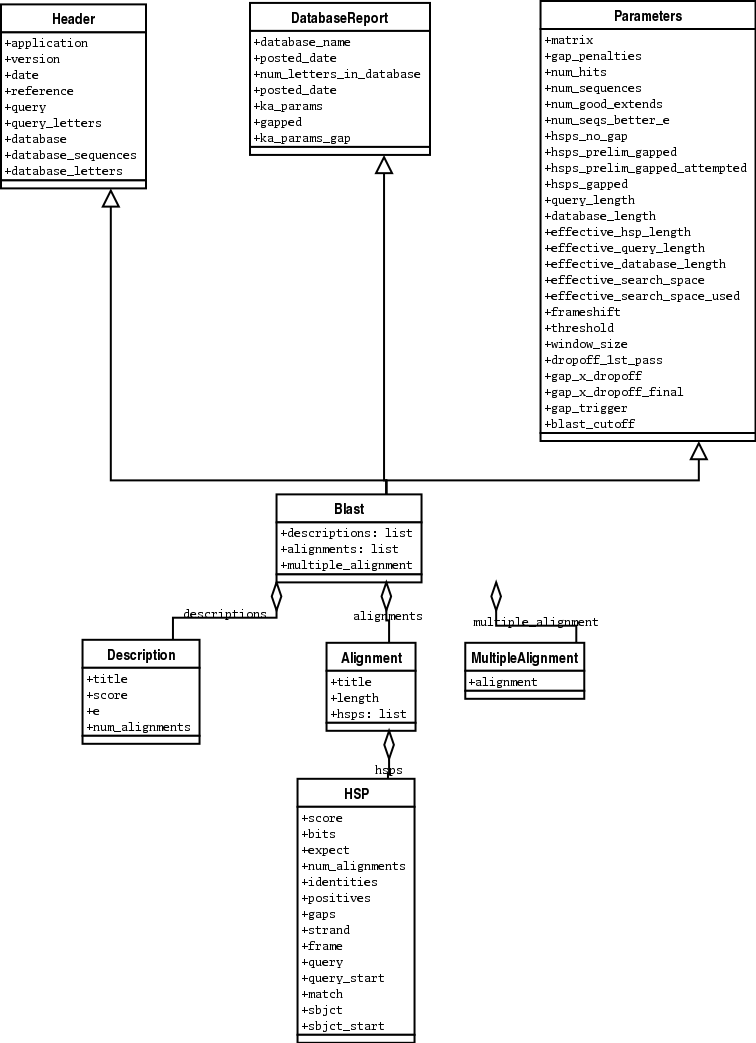
\includegraphics[width=0.8\textwidth]{images/BlastRecord.png}
\caption{Class diagram for the Blast Record class representing all of the info in a BLAST report}
\label{fig:blastrecord}
\end{figure}
\end{latexonly}

The PSIBlast record object is similar, but has support for the rounds that are used in the iteration steps of PSIBlast. The class diagram for PSIBlast is shown in Figure~\ref{fig:psiblastrecord}.

\begin{htmlonly}
\label{fig:psiblastrecord}
\imgsrc[width=650, height=750]{images/PSIBlastRecord.png}
\end{htmlonly}

\begin{latexonly}
\begin{figure}[htbp]
\centering
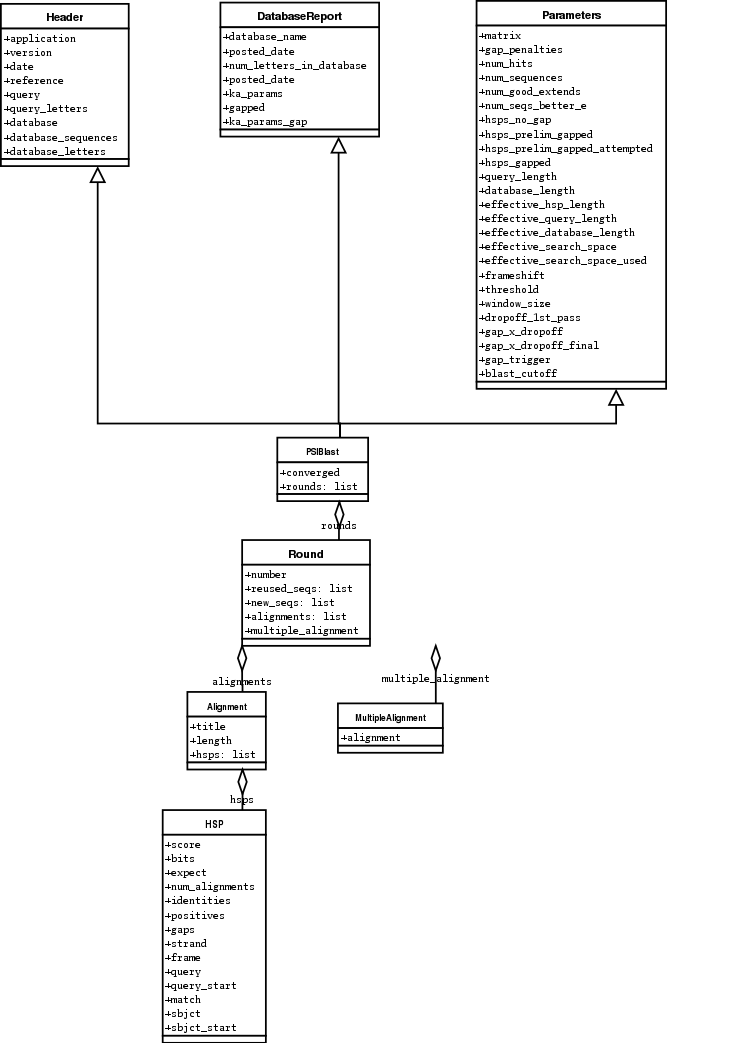
\includegraphics[width=0.8\textwidth]{images/PSIBlastRecord.png}
\caption{Class diagram for the PSIBlast Record class.}
\label{fig:psiblastrecord}
\end{figure}
\end{latexonly}

\section{Deprecated BLAST parsers}
\label{sec:parsing-blast-deprecated}

Older versions of Biopython had parsers for BLAST output in plain text or HTML
format. Over the years, we discovered that it is very hard to maintain these
parsers in working order. Basically, any small change to the BLAST output in
newly released BLAST versions tends to cause the plain text and HTML parsers
to break. We therefore recommend parsing BLAST output in XML format, as
described in section~\ref{sec:parsing-blast}.

The HTML parser in \verb|Bio.Blast.NCBIWWW| has been officially deprecated
and will issue warnings if you try and use it.  We plan to remove this
completely in a few releases time.

Our plain text BLAST parser works a bit better, but use it at your own risk.
It may or may not work, depending on which BLAST versions or programs you're
using.

\subsection{Parsing plain-text BLAST output}

The plain text BLAST parser is located in \verb|Bio.Blast.NCBIStandalone|.

As with the XML parser, we need to have a handle object that we can pass to the parser. The handle must implement the \verb|readline()| method and do this properly. The common ways to get such a handle are to either use the provided \verb|blastall| or \verb|blastpgp| functions to run the local blast, or to run a local blast via the command line, and then do something like the following:

\begin{verbatim}
>>> result_handle = open("my_file_of_blast_output.txt")
\end{verbatim}

Well, now that we've got a handle (which we'll call \verb|result_handle|),
we are ready to parse it. This can be done with the following code:

\begin{verbatim}
>>> from Bio.Blast import NCBIStandalone
>>> blast_parser = NCBIStandalone.BlastParser()
>>> blast_record = blast_parser.parse(result_handle)
\end{verbatim}

This will parse the BLAST report into a Blast Record class (either a Blast or a PSIBlast record, depending on what you are parsing) so that you can extract the information from it. In our case, let's just use print out a quick summary of all of the alignments greater than some threshold value.

\begin{verbatim}
>>> E_VALUE_THRESH = 0.04
>>> for alignment in b_record.alignments:
...     for hsp in alignment.hsps:
...         if hsp.expect < E_VALUE_THRESH:
...             print '****Alignment****'
...             print 'sequence:', alignment.title
...             print 'length:', alignment.length
...             print 'e value:', hsp.expect
...             print hsp.query[0:75] + '...'
...             print hsp.match[0:75] + '...'
...             print hsp.sbjct[0:75] + '...'
\end{verbatim}

If you also read the section~\ref{sec:parsing-blast} on parsing BLAST XML output, you'll notice that the above code is identical to what is found in that section. Once you parse something into a record class you can deal with it independent of the format of the original BLAST info you were parsing. Pretty snazzy!

Sure, parsing one record is great, but I've got a BLAST file with tons of records -- how can I parse them all? Well, fear not, the answer lies in the very next section.

\subsection{Parsing a file full of BLAST runs}

Of course, local blast is cool because you can run a whole bunch of sequences against a database and get back a nice report on all of it. So, Biopython definitely has facilities to make it easy to parse humongous files without memory problems.

We can do this using the blast iterator. To set up an iterator, we first set up a parser, to parse our blast reports in Blast Record objects:

\begin{verbatim}
>>> from Bio.Blast import NCBIStandalone
>>> blast_parser = NCBIStandalone.BlastParser()
\end{verbatim}

Then we will assume we have a handle to a bunch of blast records, which we'll call \verb|result_handle|. Getting a handle is described in full detail above in the blast parsing sections.

Now that we've got a parser and a handle, we are ready to set up the iterator with the following command:

\begin{verbatim}
>>> blast_iterator = NCBIStandalone.Iterator(blast_handle, blast_parser)
\end{verbatim}

The second option, the parser, is optional. If we don't supply a parser, then the iterator will just return the raw BLAST reports one at a time.

Now that we've got an iterator, we start retrieving blast records (generated by our parser) using \verb|next()|:

\begin{verbatim}
>>> blast_record = blast_iterator.next()
\end{verbatim}

Each call to next will return a new record that we can deal with. Now we can iterate through this records and generate our old favorite, a nice little blast report:

\begin{verbatim}
>>> for b_record in b_iterator :
...     E_VALUE_THRESH = 0.04
...     for alignment in b_record.alignments:
...         for hsp in alignment.hsps:
...             if hsp.expect < E_VALUE_THRESH:
...                 print '****Alignment****'
...                 print 'sequence:', alignment.title
...                 print 'length:', alignment.length
...                 print 'e value:', hsp.expect
...                 if len(hsp.query) > 75:
...                     dots = '...'
...                 else:
...                     dots = ''
...                 print hsp.query[0:75] + dots
...                 print hsp.match[0:75] + dots
...                 print hsp.sbjct[0:75] + dots
\end{verbatim}

%Notice that \verb|b_iterator.next()| will return \verb|None| when it runs out of records to parse, so it is easy to iterate through the entire file with a while loop that checks for the existence of a record.

The iterator allows you to deal with huge blast records without any memory problems, since things are read in one at a time. I have parsed tremendously huge files without any problems using this.

\subsection{Finding a bad record somewhere in a huge file}

One really ugly problem that happens to me is that I'll be parsing a huge blast file for a while, and the parser will bomb out with a ValueError. This is a serious problem, since you can't tell if the ValueError is due to a parser problem, or a problem with the BLAST. To make it even worse, you have no idea where the parse failed, so you can't just ignore the error, since this could be ignoring an important data point.

We used to have to make a little script to get around this problem, but the \verb|Bio.Blast| module now includes a \verb|BlastErrorParser| which really helps make this easier. The \verb|BlastErrorParser| works very similar to the regular \verb|BlastParser|, but it adds an extra layer of work by catching ValueErrors that are generated by the parser, and attempting to diagnose the errors.

Let's take a look at using this parser -- first we define the file we are going to parse and the file to write the problem reports to:

\begin{verbatim}
>>> import os
>>> blast_file = os.path.join(os.getcwd(), "blast_out", "big_blast.out")
>>> error_file = os.path.join(os.getcwd(), "blast_out", "big_blast.problems")
\end{verbatim}

Now we want to get a \verb|BlastErrorParser|:

\begin{verbatim}
>>> from Bio.Blast import NCBIStandalone
>>> error_handle = open(error_file, "w")
>>> blast_error_parser = NCBIStandalone.BlastErrorParser(error_handle)
\end{verbatim}

Notice that the parser take an optional argument of a handle. If a handle is passed, then the parser will write any blast records which generate a ValueError to this handle. Otherwise, these records will not be recorded.

Now we can use the \verb|BlastErrorParser| just like a regular blast parser. Specifically, we might want to make an iterator that goes through our blast records one at a time and parses them with the error parser:

\begin{verbatim}
>>> result_handle = open(blast_file)
>>> iterator = NCBIStandalone.Iterator(result_handle, blast_error_parser)
\end{verbatim}

We can read these records one a time, but now we can catch and deal with errors that are due to problems with Blast (and not with the parser itself):

\begin{verbatim}
>>> try:
...     next_record = iterator.next()
... except NCBIStandalone.LowQualityBlastError, info:
...     print "LowQualityBlastError detected in id %s" % info[1]
\end{verbatim}

The \verb|.next()| method is normally called indirectly via a \verb|for|-loop.
Right now the \verb|BlastErrorParser| can generate the following errors:

\begin{itemize}
  \item \verb|ValueError| -- This is the same error generated by the regular BlastParser, and is due to the parser not being able to parse a specific file. This is normally either due to a bug in the parser, or some kind of discrepancy between the version of BLAST you are using and the versions the parser is able to handle.

  \item \verb|LowQualityBlastError| -- When BLASTing a sequence that is of really bad quality (for example, a short sequence that is basically a stretch of one nucleotide), it seems that Blast ends up masking out the entire sequence and ending up with nothing to parse. In this case it will produce a truncated report that causes the parser to generate a ValueError. \verb|LowQualityBlastError| is reported in these cases. This error returns an info item with the following information:
  \begin{itemize}
    \item \verb|item[0]| -- The error message
    \item \verb|item[1]| -- The id of the input record that caused the error. This is really useful if you want to record all of the records that are causing problems.
  \end{itemize}
\end{itemize}

As mentioned, with each error generated, the BlastErrorParser will write the offending record to the specified \verb|error_handle|. You can then go ahead and look and these and deal with them as you see fit. Either you will be able to debug the parser with a single blast report, or will find out problems in your blast runs. Either way, it will definitely be a useful experience!

Hopefully the \verb|BlastErrorParser| will make it much easier to debug and deal with large Blast files.

\section{Dealing with PSIBlast}

Note that the \verb|Bio.Blast.NCBIXML| parser can read the XML output from
current versions of PSI-BLAST, but information like which sequences in each
iteration is new or reused isn't present in the XML file.
If you care about this information you may have more joy with the plain text
output and the \verb|PSIBlastParser| in \verb|Bio.Blast.NCBIStandalone|.

\chapter{Accessing NCBI's Entrez databases}
\label{chapter:entrez}

Entrez (\url{http://www.ncbi.nlm.nih.gov/Entrez}) is a data retrieval system that provides users access to NCBI's databases such as PubMed, GenBank, GEO, and many others. You can access Entrez from a web browser to manually enter queries, or you can use Biopython's \verb+Bio.Entrez+ module for programmatic access to Entrez. The latter allows you for example to search PubMed or download GenBank records from within a Python script.

The \verb+Bio.Entrez+ module makes use of the Entrez Programming Utilities (also known as EUtils), consisting of eight tools that are described in detail on NCBI's page at \url{http://www.ncbi.nlm.nih.gov/entrez/utils/}.
Each of these tools corresponds to one Python function in the \verb+Bio.Entrez+ module, as described in the sections below. This module makes sure that the correct URL is used for the queries, and that not more than one request is made every three seconds, as required by NCBI.

The output returned by the Entrez Programming Utilities is typically in XML format. To parse such output, you have several options:
\begin{enumerate}
  \item Use \verb+Bio.Entrez+'s parser to parse the XML output into a Python object;
  \item Use the DOM (Document Object Model) parser in Python's standard library;
  \item Use the SAX (Simple API for XML) parser in Python's standard library;
  \item Read the XML output as raw text, and parse it by string searching and manipulation.
\end{enumerate}
For the DOM and SAX parsers, see the Python documentation. The parser in \verb+Bio.Entrez+ is discussed below.

The Entrez Programming Utilities can also generate output in other formats, such as the Fasta or GenBank file formats for sequence databases, or the MedLine format for the literature database, discussed in Section~\ref{sec:entrez-specialized-parsers}.

\section{Entrez Guidelines}
\label{sec:entrez-guidelines}
Before using Biopython to access the NCBI's online resources (via \verb|Bio.Entrez| or some of the other modules), please read the \href{http://www.ncbi.nlm.nih.gov/entrez/query/static/eutils_help.html#UserSystemRequirements}{NCBI's Entrez User Requirements}.  If the NCBI finds you are abusing their systems, they can and will ban your access! 

To paraphrase:

\begin{itemize}
\item For any series of more than 100 requests, do this at weekends or outside USA peak times.  This is up to you to obey.
\item Use the \url{http://eutils.ncbi.nlm.nih.gov} address, not the standard NCBI Web address.  Biopython uses this web address.
\item Make no more than one request every 3 seconds.  This is automatically enforced by Biopython.
\item Use the optional email parameter so the NCBI can contact you if there is a problem.  You can either explicitly set the email address as a parameter with each call to Entrez (e.g., include {\tt email = "A.N.Other@example.com"} in the argument list), or as of Biopython 1.48, you can set a global email address:
\begin{verbatim}
>>> from Bio import Entrez
>>> Entrez.email = "A.N.Other@example.com"
\end{verbatim}
{\tt Bio.Entrez} will then use this email address with each call to Entrez.  The {\tt example.com} address is a reserved domain name specifically for documentation (RFC 2606).  Please DO NOT use a random email -- it's better not to give an email at all.
\item If you are using Biopython within some larger software suite, use the tool parameter to specify this.  The tool parameter will default to Biopython.
\item For large queries, the NCBI also recommend using their session history feature (the WebEnv session cookie string, see Section~\ref{sec:entrez-webenv}).  This is only slightly more complicated.
\end{itemize}

In conclusion, be sensible with your usage levels.  If you plan to download lots of data, consider other options.  For example, if you want easy access to all the human genes, consider fetching each chromosome by FTP as a GenBank file, and importing these into your own BioSQL database (see Section~\ref{sec:BioSQL}).

\section{EInfo: Obtaining information about the Entrez databases}

EInfo provides field index term counts, last update, and available links for each of NCBI's databases. In addition, you can use EInfo to obtain a list of all database names accessible through the Entrez utilities:
\begin{verbatim}
>>> from Bio import Entrez
>>> Entrez.email = "A.N.Other@example.com"     # Always tell NCBI who you are
>>> handle = Entrez.einfo()
>>> result = handle.read()
\end{verbatim}
The variable \verb+result+ now contains a list of databases in XML format:
\begin{verbatim}
>>> print result
<?xml version="1.0"?>
<!DOCTYPE eInfoResult PUBLIC "-//NLM//DTD eInfoResult, 11 May 2002//EN"
 "http://www.ncbi.nlm.nih.gov/entrez/query/DTD/eInfo_020511.dtd">
<eInfoResult>
<DbList>
        <DbName>pubmed</DbName>
        <DbName>protein</DbName>
        <DbName>nucleotide</DbName>
        <DbName>nuccore</DbName>
        <DbName>nucgss</DbName>
        <DbName>nucest</DbName>
        <DbName>structure</DbName>
        <DbName>genome</DbName>
        <DbName>books</DbName>
        <DbName>cancerchromosomes</DbName>
        <DbName>cdd</DbName>
        <DbName>gap</DbName>
        <DbName>domains</DbName>
        <DbName>gene</DbName>
        <DbName>genomeprj</DbName>
        <DbName>gensat</DbName>
        <DbName>geo</DbName>
        <DbName>gds</DbName>
        <DbName>homologene</DbName>
        <DbName>journals</DbName>
        <DbName>mesh</DbName>
        <DbName>ncbisearch</DbName>
        <DbName>nlmcatalog</DbName>
        <DbName>omia</DbName>
        <DbName>omim</DbName>
        <DbName>pmc</DbName>
        <DbName>popset</DbName>
        <DbName>probe</DbName>
        <DbName>proteinclusters</DbName>
        <DbName>pcassay</DbName>
        <DbName>pccompound</DbName>
        <DbName>pcsubstance</DbName>
        <DbName>snp</DbName>
        <DbName>taxonomy</DbName>
        <DbName>toolkit</DbName>
        <DbName>unigene</DbName>
        <DbName>unists</DbName>
</DbList>
</eInfoResult>
\end{verbatim}

Since this is a fairly simple XML file, we could extract the information it contains simply by string searching. Using \verb+Bio.Entrez+'s parser instead, we can directly parse this XML file into a Python object:
\begin{verbatim}
>>> from Bio import Entrez
>>> handle = Entrez.einfo()
>>> record = Entrez.read(handle)
\end{verbatim}
Now \verb+record+ is a dictionary with exactly one key:
\begin{verbatim}
>>> record.keys()
[u'DbList']
\end{verbatim}
The values stored in this key is the list of database names shown in the XML above:
\begin{verbatim}
>>> record["DbList"]
['pubmed', 'protein', 'nucleotide', 'nuccore', 'nucgss', 'nucest',
 'structure', 'genome', 'books', 'cancerchromosomes', 'cdd', 'gap',
 'domains', 'gene', 'genomeprj', 'gensat', 'geo', 'gds', 'homologene',
 'journals', 'mesh', 'ncbisearch', 'nlmcatalog', 'omia', 'omim', 'pmc',
 'popset', 'probe', 'proteinclusters', 'pcassay', 'pccompound',
 'pcsubstance', 'snp', 'taxonomy', 'toolkit', 'unigene', 'unists']
\end{verbatim}

For each of these databases, we can use EInfo again to obtain more information:
\begin{verbatim}
>>> handle = Entrez.einfo(db="pubmed")
>>> record = Entrez.read(handle)
>>> record["DbInfo"]["Description"]
'PubMed bibliographic record'
>>> record["DbInfo"]["Count"]
'17989604'
>>> record["DbInfo"]["LastUpdate"]
'2008/05/24 06:45'
\end{verbatim}
Try \verb+record["DbInfo"].keys()+ for other information stored in this record.

\section{ESearch: Searching the Entrez databases}
\label{sec:entrez-esearch}
To search any of these databases, we use \verb+Bio.Entrez.esearch()+. For example, let's search in PubMed for publications related to Biopython:
\begin{verbatim}
>>> from Bio import Entrez
>>> Entrez.email = "A.N.Other@example.com"     # Always tell NCBI who you are
>>> handle = Entrez.esearch(db="pubmed", term="biopython")
>>> record = Entrez.read(handle)
>>> record["IdList"]
['16403221', '16377612', '14871861', '14630660', '12230038']
\end{verbatim}
In this output, you see five PubMed IDs (16403221, 16377612, 14871861, 14630660, 12230038), which can be retrieved by EFetch (see section \ref{sec:efetch}).

You can also use ESearch to search GenBank. Here we'll do a quick search for the \emph{matK} gene in \emph{Cypripedioideae} orchids:

\begin{verbatim}
>>> handle = Entrez.esearch(db="nucleotide",term="Cypripedioideae[Orgn] AND matK[Gene]")
>>> record = Entrez.read(handle)
>>> record["Count"]
'25'
>>> record["IdList"]
['186972394', '186972384', '186972382', '186972378', ..., '61585484']
\end{verbatim}
Each of the IDs (186972394, 186972384, 186972382, \ldots) is a GenBank identifier. See section~\ref{sec:efetch} for information on how to actually download these GenBank records.

As a final example, let's get a list of computational journal titles:
\begin{verbatim}
>>> handle = Entrez.esearch(db="journals", term="computational")
>>> record = Entrez.read(handle)
>>> record["Count"]
'16'
>>> record["IdList"]
['30367', '33843', '33823', '32989', '33190', '33009', '31986',
 '34502', '8799', '22857', '32675', '20258', '33859', '32534',
 '32357', '32249']
\end{verbatim}
Again, we could use EFetch to obtain more information for each of these journal IDs.

ESearch has many useful options --- see the \href{http://www.ncbi.nlm.nih.gov/entrez/query/static/esearch\_help.html}{ESearch help page} for more information.

\section{EPost}
EPost posts a list of UIs for use in subsequent search strategies; see the  \href{http://www.ncbi.nlm.nih.gov/entrez/query/static/epost\_help.html}{EPost help page} for more information. It is available from Biopython through \verb+Bio.Entrez.epost()+.

\section{ESummary: Retrieving summaries from primary IDs}
ESummary retrieves document summaries from a list of primary IDs (see the  \href{http://www.ncbi.nlm.nih.gov/entrez/query/static/esummary\_help.html}{ESummary help page} for more information). In Biopython, ESummary is available as \verb+Bio.Entrez.esummary()+. Using the search result above, we can for example find out more about the journal with ID 30367:
\begin{verbatim}
>>> from Bio import Entrez
>>> Entrez.email = "A.N.Other@example.com"     # Always tell NCBI who you are
>>> handle = Entrez.esummary(db="journals", id="30367")
>>> record = Entrez.read(handle)
>>> record[0]["Id"]
'30367'
>>> record[0]["Title"]
'Computational biology and chemistry'
>>> record[0]["Publisher"]
'Pergamon,'
\end{verbatim}

\section{EFetch: Downloading full records from Entrez}
\label{sec:efetch}

EFetch is what you use when you want to retrieve a full record from Entrez.
From the \emph{Cypripedioideae} example above, we can download GenBank record 186972394 using \verb+Bio.Entrez.efetch+:

\begin{verbatim}
>>> from Bio import Entrez
>>> Entrez.email = "A.N.Other@example.com"     # Always tell NCBI who you are
>>> handle = Entrez.efetch(db="nucleotide", id="186972394", rettype="genbank")
>>> print handle.read()
LOCUS       EU490707                1302 bp    DNA     linear   PLN 05-MAY-2008
DEFINITION  Selenipedium aequinoctiale maturase K (matK) gene, partial cds;
            chloroplast.
ACCESSION   EU490707
VERSION     EU490707.1  GI:186972394
KEYWORDS    .
SOURCE      chloroplast Selenipedium aequinoctiale
  ORGANISM  Selenipedium aequinoctiale
            Eukaryota; Viridiplantae; Streptophyta; Embryophyta; Tracheophyta;
            Spermatophyta; Magnoliophyta; Liliopsida; Asparagales; Orchidaceae;
            Cypripedioideae; Selenipedium.
REFERENCE   1  (bases 1 to 1302)
  AUTHORS   Neubig,K.M., Whitten,W.M., Carlsward,B.S., Blanco,M.A.,
            Endara,C.L., Williams,N.H. and Moore,M.J.
  TITLE     Phylogenetic utility of ycf1 in orchids
  JOURNAL   Unpublished
REFERENCE   2  (bases 1 to 1302)
  AUTHORS   Neubig,K.M., Whitten,W.M., Carlsward,B.S., Blanco,M.A.,
            Endara,C.L., Williams,N.H. and Moore,M.J.
  TITLE     Direct Submission
  JOURNAL   Submitted (14-FEB-2008) Department of Botany, University of
            Florida, 220 Bartram Hall, Gainesville, FL 32611-8526, USA
FEATURES             Location/Qualifiers
     source          1..1302
                     /organism="Selenipedium aequinoctiale"
                     /organelle="plastid:chloroplast"
                     /mol_type="genomic DNA"
                     /specimen_voucher="FLAS:Blanco 2475"
                     /db_xref="taxon:256374"
     gene            <1..>1302
                     /gene="matK"
     CDS             <1..>1302
                     /gene="matK"
                     /codon_start=1
                     /transl_table=11
                     /product="maturase K"
                     /protein_id="ACC99456.1"
                     /db_xref="GI:186972395"
                     /translation="IFYEPVEIFGYDNKSSLVLVKRLITRMYQQNFLISSVNDSNQKG
                     FWGHKHFFSSHFSSQMVSEGFGVILEIPFSSQLVSSLEEKKIPKYQNLRSIHSIFPFL
                     EDKFLHLNYVSDLLIPHPIHLEILVQILQCRIKDVPSLHLLRLLFHEYHNLNSLITSK
                     KFIYAFSKRKKRFLWLLYNSYVYECEYLFQFLRKQSSYLRSTSSGVFLERTHLYVKIE
                     HLLVVCCNSFQRILCFLKDPFMHYVRYQGKAILASKGTLILMKKWKFHLVNFWQSYFH
                     FWSQPYRIHIKQLSNYSFSFLGYFSSVLENHLVVRNQMLENSFIINLLTKKFDTIAPV
                     ISLIGSLSKAQFCTVLGHPISKPIWTDFSDSDILDRFCRICRNLCRYHSGSSKKQVLY
                     RIKYILRLSCARTLARKHKSTVRTFMRRLGSGLLEEFFMEEE"
ORIGIN      
        1 attttttacg aacctgtgga aatttttggt tatgacaata aatctagttt agtacttgtg
       61 aaacgtttaa ttactcgaat gtatcaacag aattttttga tttcttcggt taatgattct
      121 aaccaaaaag gattttgggg gcacaagcat tttttttctt ctcatttttc ttctcaaatg
      181 gtatcagaag gttttggagt cattctggaa attccattct cgtcgcaatt agtatcttct
      241 cttgaagaaa aaaaaatacc aaaatatcag aatttacgat ctattcattc aatatttccc
      301 tttttagaag acaaattttt acatttgaat tatgtgtcag atctactaat accccatccc
      361 atccatctgg aaatcttggt tcaaatcctt caatgccgga tcaaggatgt tccttctttg
      421 catttattgc gattgctttt ccacgaatat cataatttga atagtctcat tacttcaaag
      481 aaattcattt acgccttttc aaaaagaaag aaaagattcc tttggttact atataattct
      541 tatgtatatg aatgcgaata tctattccag tttcttcgta aacagtcttc ttatttacga
      601 tcaacatctt ctggagtctt tcttgagcga acacatttat atgtaaaaat agaacatctt
      661 ctagtagtgt gttgtaattc ttttcagagg atcctatgct ttctcaagga tcctttcatg
      721 cattatgttc gatatcaagg aaaagcaatt ctggcttcaa agggaactct tattctgatg
      781 aagaaatgga aatttcatct tgtgaatttt tggcaatctt attttcactt ttggtctcaa
      841 ccgtatagga ttcatataaa gcaattatcc aactattcct tctcttttct ggggtatttt
      901 tcaagtgtac tagaaaatca tttggtagta agaaatcaaa tgctagagaa ttcatttata
      961 ataaatcttc tgactaagaa attcgatacc atagccccag ttatttctct tattggatca
     1021 ttgtcgaaag ctcaattttg tactgtattg ggtcatccta ttagtaaacc gatctggacc
     1081 gatttctcgg attctgatat tcttgatcga ttttgccgga tatgtagaaa tctttgtcgt
     1141 tatcacagcg gatcctcaaa aaaacaggtt ttgtatcgta taaaatatat acttcgactt
     1201 tcgtgtgcta gaactttggc acggaaacat aaaagtacag tacgcacttt tatgcgaaga
     1261 ttaggttcgg gattattaga agaattcttt atggaagaag aa
//
\end{verbatim}

The argument \verb+rettype="genbank"+ lets us download this record in the GenBank format. Alternatively, you could for example use \verb+rettype="fasta"+ to get the Fasta-format; see the \href{http://www.ncbi.nlm.nih.gov/entrez/query/static/efetchseq\_help.html}{EFetch Help page} for other options. The available formats depend on which database you are downloading from.

If you fetch the record in one of the formats accepted by \verb+Bio.SeqIO+ (see Chapter~\ref{chapter:Bio.SeqIO}), you can directly parse it into a \verb+SeqRecord+:

\begin{verbatim}
>>> from Bio import Entrez, SeqIO
>>> handle = Entrez.efetch(db="nucleotide", id="186972394",rettype="genbank")
>>> record = SeqIO.read(handle, "genbank")
>>> print record
ID: EU490707.1
Name: EU490707
Description: Selenipedium aequinoctiale maturase K (matK) gene, partial cds; chloroplast.
Number of features: 3
...
Seq('ATTTTTTACGAACCTGTGGAAATTTTTGGTTATGACAATAAATCTAGTTTAGTA...GAA', IUPACAmbiguousDNA())\end{verbatim}

To get the output in XML format, which you can parse using the \verb+Bio.Entrez.read()+ function, use \verb+retmode="xml"+:

\begin{verbatim}
>>> from Bio import Entrez
>>> handle = Entrez.efetch(db="nucleotide", id="186972394", retmode="xml")
>>> record = Entrez.read(handle)
>>> record[0]["GBSeq_definition"] 
'Selenipedium aequinoctiale maturase K (matK) gene, partial cds; chloroplast'
>>> record[0]["GBSeq_source"] 
'chloroplast Selenipedium aequinoctiale'
\end{verbatim}

If you want to perform a search with \verb|Bio.Entrez.esearch()|, and then download the records with \verb|Bio.Entrez.efetch()|, you should use the WebEnv history feature -- see Section~\ref{sec:entrez-webenv}.

\section{ELink}
For help on ELink, see the \href{http://www.ncbi.nlm.nih.gov/entrez/query/static/elink\_help.html}{ELink help page}. ELink is available from Biopython through \verb+Bio.Entrez.elink()+.

\section{EGQuery: Obtaining counts for search terms}
EGQuery provides counts for a search term in each of the Entrez databases. This is particularly useful to find out how many items your search terms would find in each database without actually performing lots of separate searches with ESearch (see the example in \ref{subsec:entrez_example_genbank} below).

In this example, we use \verb+Bio.Entrez.egquery()+ to obtain the counts for ``Biopython'':

\begin{verbatim}
>>> from Bio import Entrez
>>> Entrez.email = "A.N.Other@example.com"     # Always tell NCBI who you are
>>> handle = Entrez.egquery(term="biopython")
>>> record = Entrez.read(handle)
>>> for row in record["eGQueryResult"]: print row["DbName"], row["Count"]
...
pubmed 6
pmc 62
journals 0
...
\end{verbatim}
See the \href{http://www.ncbi.nlm.nih.gov/entrez/query/static/egquery\_help.html}{EGQuery help page} for more information.

\section{ESpell: Obtaining spelling suggestions}
ESpell retrieves spelling suggestions. In this example, we use \verb+Bio.Entrez.espell()+ to obtain the correct spelling of Biopython:

\begin{verbatim}
>>> from Bio import Entrez
>>> Entrez.email = "A.N.Other@example.com"     # Always tell NCBI who you are
>>> handle = Entrez.espell(term="biopythooon")
>>> record = Entrez.read(handle)
>>> record["Query"]
'biopythooon'
>>> record["CorrectedQuery"]
'biopython'
\end{verbatim}
See the \href{http://www.ncbi.nlm.nih.gov/entrez/query/static/espell\_help.html}{ESpell help page} for more information.

\section{Specialized parsers}
\label{sec:entrez-specialized-parsers}

The \verb+Bio.Entrez.read+ function can parse most (if not all) XML output returned by Entrez. Entrez typically allows you to retrieve records in other formats, which may have some advantages compared to the XML format in terms of readability.

To request a specific file format from Entrez using \verb|Bio.Entrez.efetch()| requires specifying the \verb|rettype| and/or \verb|retmode| optional arguments.  The different combinations are described for each database type on the \href{http://www.ncbi.nlm.nih.gov/entrez/query/static/efetch_help.html}{NCBI efetch webpage}.

One obvious case is you may prefer to download sequences in the FASTA or GenBank plain text formats (which can then be parsed with \verb|Bio.SeqIO|, see Sections~\ref{sec:SeqIO_GenBank_Online} and~\ref{sec:efetch}).  For the literature databases, Biopython contains a parser for the \verb+MEDLINE+ format used in PubMed.

\subsection{Parsing Medline records}
\label{subsec:entrez-and-medline}
You can find the Medline parser in \verb+Bio.Medline+. Suppose we want to parse the file \verb+pubmed_result1.txt+, containing one Medline record. You can find this file in Biopython's \verb+Tests\Medline+ directory. The file looks like this:

\begin{verbatim}
PMID- 12230038
OWN - NLM
STAT- MEDLINE
DA  - 20020916
DCOM- 20030606
LR  - 20041117
PUBM- Print
IS  - 1467-5463 (Print)
VI  - 3
IP  - 3
DP  - 2002 Sep
TI  - The Bio* toolkits--a brief overview.
PG  - 296-302
AB  - Bioinformatics research is often difficult to do with commercial software. The
      Open Source BioPerl, BioPython and Biojava projects provide toolkits with
...
\end{verbatim}We first open the file and then parse it:
\begin{verbatim}
>>> from Bio import Medline
>>> input = open("pubmed_result1.txt")
>>> record = Medline.read(input)
\end{verbatim}
The \verb+record+ now contains the Medline record as a Python dictionary:
\begin{verbatim}
>>> record["PMID"]
'12230038'
>>> record["AB"]
'Bioinformatics research is often difficult to do with commercial software.
The Open Source BioPerl, BioPython and Biojava projects provide toolkits with
multiple functionality that make it easier to create customised pipelines or
analysis. This review briefly compares the quirks of the underlying languages
and the functionality, documentation, utility and relative advantages of the
Bio counterparts, particularly from the point of view of the beginning
biologist programmer.'
\end{verbatim}
The key names used in a Medline record can be rather obscure; use
\begin{verbatim}
>>> help(record)
\end{verbatim}
for a brief summary.

To parse a file containing multiple Medline records, you can use the \verb+parse+ function instead:
\begin{verbatim}
>>> from Bio import Medline
>>> input = open("pubmed_result2.txt")
>>> records = Medline.parse(input)
>>> for record in records:
...     print record["TI"]
A high level interface to SCOP and ASTRAL implemented in python.
GenomeDiagram: a python package for the visualization of large-scale genomic data.
Open source clustering software.
PDB file parser and structure class implemented in Python.
\end{verbatim}

Instead of parsing Medline records stored in files, you can also parse Medline records downloaded by \verb+Bio.Entrez.efetch+. For example, let's look at all Medline records in PubMed related to Biopython:
\begin{verbatim}
>>> from Bio import Entrez
>>> Entrez.email = "A.N.Other@example.com"     # Always tell NCBI who you are
>>> handle = Entrez.esearch(db="pubmed",term="biopython")
>>> record = Entrez.read(handle)
>>> record["IdList"]
['18606172', '16403221', '16377612', '14871861', '14630660', '12230038']
\end{verbatim}
We now use \verb+Bio.Entrez.efetch+ to download these Medline records:
\begin{verbatim}
>>> idlist = record["IdList"]
>>> handle = Entrez.efetch(db="pubmed",id=idlist,rettype="medline",retmode="text")
\end{verbatim}
Here, we specify \verb+rettype="medline", retmode="text"+ to obtain the Medline records in plain-text Medline format. Now we use \verb+Bio.Medline+ to parse these records:
\begin{verbatim}
>>> from Bio import Medline
>>> records = Medline.parse(handle)
>>> for record in records:
...     print record["AU"]
['Munteanu CR', 'Gonzalez-Diaz H', 'Magalhaes AL']
['Casbon JA', 'Crooks GE', 'Saqi MA']
['Pritchard L', 'White JA', 'Birch PR', 'Toth IK']
['de Hoon MJ', 'Imoto S', 'Nolan J', 'Miyano S']
['Hamelryck T', 'Manderick B']
['Mangalam H']
\end{verbatim}

For comparison, here we show an example using the XML format:
\begin{verbatim}
>>> idlist = record["IdList"]
>>> handle = Entrez.efetch(db="pubmed",id=idlist,rettype="medline",retmode="xml")
>>> records = Entrez.read(handle)
>>> for record in records:
...     print record["MedlineCitation"]["Article"]["ArticleTitle"]
Enzymes/non-enzymes classification model complexity based on composition, sequence, 3D
 and topological indices.
A high level interface to SCOP and ASTRAL implemented in python.
GenomeDiagram: a python package for the visualization of large-scale genomic data.
Open source clustering software.
PDB file parser and structure class implemented in Python.
The Bio* toolkits--a brief overview.
\end{verbatim}

\section{Examples}
\label{sec:entrez_examples}

\subsection{PubMed and Medline}
\label{subsec:pub_med}

If you are in the medical field or interested in human issues (and many times even if you are not!), PubMed (\url{http://www.ncbi.nlm.nih.gov/PubMed/}) is an excellent source of all kinds of goodies. So like other things, we'd like to be able to grab information from it and use it in python scripts.

In this example, we will query PubMed for all articles having to do with orchids (see section~\ref{sec:orchids} for our motivation). We first check how many of such articles there are:

\begin{verbatim}
>>> from Bio import Entrez
>>> Entrez.email = "A.N.Other@example.com"     # Always tell NCBI who you are
>>> handle = Entrez.egquery(term="orchid")
>>> record = Entrez.read(handle)
>>> for row in record["eGQueryResult"]:
...     if row["DbName"]=="pubmed":
...         print row["Count"]
463
\end{verbatim}

Now we use the \verb+Bio.Entrez.efetch+ function to download the PubMed IDs of these 463 articles:
\begin{verbatim}
>>> handle = Entrez.esearch(db="pubmed", term="orchid", retmax=463)
>>> record = Entrez.read(handle)
>>> idlist = record["IdList"]
>>> print idlist
\end{verbatim}


This returns a python list containing all of the PubMed IDs of articles related to orchids:

\begin{verbatim}
['18680603', '18665331', '18661158', '18627489', '18627452', '18612381',
'18594007', '18591784', '18589523', '18579475', '18575811', '18575690',
...
\end{verbatim}

Now that we've got them, we obviously want to get the corresponding Medline records and extract the information from them. Here, we'll download the Medline records in the Medline flat-file format, and use the \verb+Bio.Medline+ module to parse them:

\begin{verbatim}
>>> from Bio import Medline
>>> handle = Entrez.efetch(db="pubmed", id=idlist, rettype="medline",
                           retmode="text")
>>> records = Medline.parse(handle)
\end{verbatim}

Keep in mind that \verb+records+ is an iterator, so you can iterate through the records only once. If you want to save the records, you can convert them to a list:

\begin{verbatim}
>>> records = list(records)
\end{verbatim}

Let's now iterate over the records to print out some information about each record:

\begin{verbatim}
>>> for record in records:
...     print "title:", record["TI"]
...     if "AU" in records:
...         print "authors:", record["AU"]
...     print "source:", record["CO"]
...     print
\end{verbatim}

The output for this looks like:

\begin{verbatim}
title: Sex pheromone mimicry in the early spider orchid (ophrys sphegodes):
patterns of hydrocarbons as the key mechanism for pollination by sexual
deception [In Process Citation]
authors: ['Schiestl FP', 'Ayasse M', 'Paulus HF', 'Lofstedt C', 'Hansson BS',
'Ibarra F', 'Francke W']
source: J Comp Physiol [A] 2000 Jun;186(6):567-74
\end{verbatim}

Especially interesting to note is the list of authors, which is returned as a standard python list. This makes it easy to manipulate and search using standard python tools. For instance, we could loop through a whole bunch of entries searching for a particular author with code like the following:

\begin{verbatim}
>>> search_author = "Waits T"

>>> for record in records:
...     if not "AU" in record:
...         continue
...     if search_author in record["	AU"]:
...         print "Author %s found: %s" % (search_author, record["SO"])
\end{verbatim}

Hopefully this section gave you an idea of the power and flexibility of the Entrez and Medline interfaces and how they can be used together.

\subsection{Searching, downloading, and parsing Entrez Nucleotide records with Bio.Entrez}
\label{subsec:entrez_example_genbank}

Here we'll show a simple example of performing a remote Entrez query. In section~\ref{sec:orchids} of the parsing examples, we talked about using NCBI's Entrez website to search the NCBI nucleotide databases for info on Cypripedioideae, our friends the lady slipper orchids. Now, we'll look at how to automate that process using a Python script. In this example, we'll just show how to connect, get the results, and parse them, with the Entrez module doing all of the work.

First, we use EGQuery to find out the number of results we will get before actually downloading them.  EGQuery will tell us how many search results were found in each of the databases, but for this example we are only interested in nucleotides:
\begin{verbatim}
>>> from Bio import Entrez
>>> Entrez.email = "A.N.Other@example.com"     # Always tell NCBI who you are
>>> handle = Entrez.egquery(term="Cypripedioideae")
>>> record = Entrez.read(handle)
>>> for row in record["eGQueryResult"]:
...     if row["DbName"]=="nuccore":
...         print row["Count"]
814
\end{verbatim}

So, we expect to find 814 Entrez Nucleotide records (this is the number I obtained in 2008; it is likely to increase in the future). If you find some ridiculously high number of hits, you may want to reconsider if you really want to download all of them, which is our next step:
\begin{verbatim}
>>> from Bio import Entrez
>>> handle = Entrez.esearch(db="nucleotide", term="Cypripedioideae", retmax=814)
>>> record = Entrez.read(handle)
\end{verbatim}

Here, \verb+record+ is a Python dictionary containing the search results and some auxiliary information. Just for information, let's look at what is stored in this dictionary:
\begin{verbatim}
>>> print record.keys()
[u'Count', u'RetMax', u'IdList', u'TranslationSet', u'RetStart', u'QueryTranslation']
\end{verbatim}
First, let's check how many results were found:
\begin{verbatim}
>>> print record["Count"]
'814'
\end{verbatim}
which is the number we expected. The 814 results are stored in \verb+record['IdList']+:
\begin{verbatim}
>>> print len(record["IdList"])
814
\end{verbatim}
Let's look at the first five results:
\begin{verbatim}
>>> print record["IdList"][:5]
['187237168', '187372713', '187372690', '187372688', '187372686']
\end{verbatim}

\label{sec:entrez-batched-efetch}
We can download these records using \verb+efetch+.
While you could download these records one by one, to reduce the load on NCBI's servers, it is better to fetch a bunch of records at the same time, shown below.
However, in this situation you should ideally be using the history feature described later in Section~\ref{sec:entrez-webenv}.

\begin{verbatim}
>>> idlist = ",".join(record["IdList"][:5])
>>> print idlist
187237168,187372713,187372690,187372688,187372686
>>> handle = Entrez.efetch(db="nucleotide", id=idlist, retmode="xml")
>>> records = Entrez.read(handle)
>>> print len(records)
5
\end{verbatim}
Each of these records corresponds to one GenBank record.
\begin{verbatim}
>>> print records[0].keys()
[u'GBSeq_moltype', u'GBSeq_source', u'GBSeq_sequence',
 u'GBSeq_primary-accession', u'GBSeq_definition', u'GBSeq_accession-version',
 u'GBSeq_topology', u'GBSeq_length', u'GBSeq_feature-table',
 u'GBSeq_create-date', u'GBSeq_other-seqids', u'GBSeq_division',
 u'GBSeq_taxonomy', u'GBSeq_references', u'GBSeq_update-date',
 u'GBSeq_organism', u'GBSeq_locus', u'GBSeq_strandedness']

>>> print records[0]["GBSeq_primary-accession"]
DQ110336

>>> print records[0]["GBSeq_other-seqids"]
['gb|DQ110336.1|', 'gi|187237168']

>>> print records[0]["GBSeq_definition"]
Cypripedium calceolus voucher Davis 03-03 A maturase (matR) gene, partial cds;
mitochondrial

>>> print records[0]["GBSeq_organism"]
Cypripedium calceolus
\end{verbatim}

You could use this to quickly set up searches -- but for heavy usage, see Section~\ref{sec:entrez-webenv}.

\subsection{Searching, downloading, and parsing GenBank records using Bio.Entrez and Bio.SeqIO}
\label{sec:entrez-search-fetch-genbank}

The GenBank record format is a very popular method of holding information about sequences, sequence features, and other associated sequence information. The format is a good way to get information from the NCBI databases at \url{http://www.ncbi.nlm.nih.gov/}.

In this example we'll show how to query the NCBI databases,to retrieve the records from the query, and then parse them using \verb+Bio.SeqIO+  - something touched on in Section~\ref{sec:SeqIO_GenBank_Online}.

For simplicity, this example \emph{does not} take advantage of the WebEnv history feature -- see Section~\ref{sec:entrez-webenv} for this.

First, we want to make a query and find out the ids of the records to retrieve. Here we'll do a quick search for one of our favorite organisms, \emph{Opuntia} (prickly-pear cacti). We can do quick search and get back the GIs (GenBank identifiers) for all of the corresponding records. First we check how many records there are:

\begin{verbatim}
>>> from Bio import Entrez
>>> Entrez.email = "A.N.Other@example.com"     # Always tell NCBI who you are
>>> handle = Entrez.egquery(term="Opuntia AND rpl16")
>>> record = Entrez.read(handle)
>>> for row in record["eGQueryResult"]:
...     if row["DbName"]=="nuccore":
...         print row["Count"]
...
9
\end{verbatim}
Now we download the list of GenBank identifiers:
\begin{verbatim}
>>> handle = Entrez.esearch(db="nuccore", term="Opuntia AND rpl16")
>>> record = Entrez.read(handle)
>>> gi_list = record["IdList"]
>>> gi_list
['57240072', '57240071', '6273287', '6273291', '6273290', '6273289', '6273286',
'6273285', '6273284']
\end{verbatim}

Now we use these GIs to download the GenBank records - note that you have to supply a comma separated list of GI numbers to Entrez:

\begin{verbatim}
>>> gi_str = ",".join(gi_list)
>>> handle = Entrez.efetch(db="nuccore", id=gi_str, rettype="genbank")
\end{verbatim}

If you want to look at the raw GenBank files, you can read from this handle and print out the result:

\begin{verbatim}
>>> text = handle.read()
>>> print text
LOCUS       AY851612                 892 bp    DNA     linear   PLN 10-APR-2007
DEFINITION  Opuntia subulata rpl16 gene, intron; chloroplast.
ACCESSION   AY851612
VERSION     AY851612.1  GI:57240072
KEYWORDS    .
SOURCE      chloroplast Austrocylindropuntia subulata
  ORGANISM  Austrocylindropuntia subulata
            Eukaryota; Viridiplantae; Streptophyta; Embryophyta; Tracheophyta;
            Spermatophyta; Magnoliophyta; eudicotyledons; core eudicotyledons;
            Caryophyllales; Cactaceae; Opuntioideae; Austrocylindropuntia.
REFERENCE   1  (bases 1 to 892)
  AUTHORS   Butterworth,C.A. and Wallace,R.S.
...
\end{verbatim}

In this case, we are just getting the raw records. To get the records in a more Python-friendly form, we can use \verb+Bio.SeqIO+ to parse the GenBank data into \verb|SeqRecord| objects, including \verb|SeqFeature| objects (see Chapter~\ref{chapter:Bio.SeqIO}):

\begin{verbatim}
>>> from Bio import SeqIO
>>> handle = Entrez.efetch(db="nuccore", id=gi_str, rettype="genbank")
>>> records = SeqIO.parse(handle, "genbank")
\end{verbatim}

\noindent We can now step through the records and look at the information we are interested in:
\begin{verbatim}
>>> for record in records: 
>>> ...    print "%s, length %i, with %i features" \
>>> ...           % (record.name, len(record), len(record.features))
AY851612, length 892, with 3 features
AY851611, length 881, with 3 features
AF191661, length 895, with 3 features
AF191665, length 902, with 3 features
AF191664, length 899, with 3 features
AF191663, length 899, with 3 features
AF191660, length 893, with 3 features
AF191659, length 894, with 3 features
AF191658, length 896, with 3 features
\end{verbatim}

Using these automated query retrieval functionality is a big plus over doing things by hand.   Although the module should obey the NCBI's three-second rule, the NCBI have other recommendations like avoiding peak hours.  See Section~\ref{sec:entrez-guidelines}.
In particular, please note that for simplicity, this example does not use the WebEnv history feature.  You should use this for any non-trivial search and download work, see Section~\ref{sec:entrez-webenv}.

Finally, if plan to repeat your analysis, rather than downloading the files from the NCBI and parsing them immediately, consider just downloading the files \emph{once} and saving them to your hard disk.

\subsection{Finding the lineage of an organism}

Staying with the same organism, let's now find its lineage. First, we search the Taxonomy database for Cypripedioideae (an orchid family). We find exactly one accession number:
\begin{verbatim}
>>> from Bio import Entrez
>>> Entrez.email = "A.N.Other@example.com"     # Always tell NCBI who you are
>>> handle = Entrez.esearch(db="Taxonomy", term="Cypripedioideae")
>>> record = Entrez.read(handle)
>>> record["IdList"]
['158330']
>>> record["IdList"][0]
'158330'
\end{verbatim}
Now, we use \verb+efetch+ to download this entry in the Taxonomy database and to parse it:
\begin{verbatim}
>>> handle = Entrez.efetch(db="Taxonomy", id="158330", retmode="xml")
>>> records = Entrez.read(handle)
\end{verbatim}
Again, this record stores lots of information:
\begin{verbatim}
>>> records[0].keys()
[u'Lineage', u'Division', u'ParentTaxId', u'PubDate', u'LineageEx',
 u'CreateDate', u'TaxId', u'Rank', u'GeneticCode', u'ScientificName',
 u'MitoGeneticCode', u'UpdateDate']
\end{verbatim}
We can get the lineage directly from this record:
\begin{verbatim}
>>> records[0]["Lineage"]
'cellular organisms; Eukaryota; Viridiplantae; Streptophyta; Streptophytina;
 Embryophyta; Tracheophyta; Euphyllophyta; Spermatophyta; Magnoliophyta;
 Liliopsida; Asparagales; Orchidaceae'
\end{verbatim}

\section{Using the history and WebEnv}
\label{sec:entrez-webenv}

Often you will want to make a series of linked queries.  Most typically, running a search, perhaps refining the search, and then retrieving detailed search results.  You \emph{can} do this by making a series of separate calls to Entrez.  However, the NCBI prefer you to take advantage of their history support.

\subsection{Searching for and downloading sequences using the history}
For example, suppose we want to search and download all the \textit{Opuntia} rpl16 nucleotide sequences, and store them in a FASTA file.  As shown in Section~\ref{sec:entrez-search-fetch-genbank}, we can naively combine \verb|Bio.Entrez.esearch()| (Section~\ref{sec:entrez-esearch}) to get a list of GI numbers, and then call \verb|Bio.Entrez.efetch()| (Section~\ref{sec:efetch}) to download them all.

However, the approved approach is to run the search with the history feature.  Then, we can fetch the results by reference to the search results - which the NCBI can anticipate and cache.

To do this, you call \verb|Bio.Entrez.esearch()| as normal, but with the additional argument of \verb|usehistory="y"|,

\begin{verbatim}
>>> from Bio import Entrez
>>> Entrez.email = "history.user@example.com"
>>> search_handle = Entrez.esearch(db="nucleotide",term="Opuntia and rpl16",
                                   usehistory="y")
>>> search_results = Entrez.read(search_handle)
>>> search_handle.close()
\end{verbatim}

\noindent When you get the XML output back, it will still include the usual search results:

\begin{verbatim}
>>> gi_list = search_results["IdList"]
>>> count = int(search_results["Count"])
>>> assert count == len(gi_list)
\end{verbatim}

\noindent However, you also get given two additional pieces of information, the {\tt WebEnv} session cookie, and the{\tt QueryKey}:

\begin{verbatim}
>>> session_cookie = search_results["WebEnv"]
>>> query_key = search_results["QueryKey"] 
\end{verbatim}

Having stored these values in variables {\tt session\_cookie} and {\tt query\_key} we can use them as parameters to \verb|Bio.Entrez.efetch()| instead of giving the GI numbers as identifiers.  

While for small searches you might be OK downloading everything at once, its better download in batches.  You use the {\tt retstart} and {\tt retmax} parameters to specify which range of search results you want returned (starting entry using zero-based counting, and maximum number of results to return).  For example,

\begin{verbatim}
batch_size = 3
out_handle = open("orchid_rpl16.fasta", "w")
for start in range(0,count,batch_size) :
    end = min(count, start+batch_size)
    print "Going to download record %i to %i" % (start+1, end)
    fetch_handle = Entrez.efetch(db="nucleotide", rettype="fasta",
                                 retstart=start, retmax=batch_size,
                                 webenv=session_cookie, query_key=query_key)
    data = fetch_handle.read()
    fetch_handle.close()
    out_handle.write(data)
out_handle.close()
\end{verbatim}

\noindent For illustrative purposes, this example downloaded the FASTA records in batches of three.  Unless you are downloading genomes or chromosomes, you would normally pick a larger batch size.

\subsection{Searching for and downloading abstracts using the history}
Here is another history example, searching for papers published in the last year about the \textit{Opuntia}, and then download them into a file in MedLine format:

\begin{verbatim}
from Bio import Entrez
Entrez.email = "history.user@example.com"
search_results = Entrez.read(Entrez.esearch(db="pubmed",
                                            term="Opuntia[ORGN]",
                                            reldate=365, datetype="pdat",
                                            usehistory="y"))
count = int(search_results["Count"])
print "Found %i results" % count

batch_size = 10
out_handle = open("recent_orchid_papers.txt", "w")
for start in range(0,count,batch_size) :
    end = min(count, start+batch_size)
    print "Going to download record %i to %i" % (start+1, end)
    fetch_handle = Entrez.efetch(db="pubmed", rettype="medline",
                                 retstart=start, retmax=batch_size,
                                 webenv=search_results["WebEnv"],
                                 query_key=search_results["QueryKey"])
    data = fetch_handle.read()
    fetch_handle.close()
    out_handle.write(data)
out_handle.close()
\end{verbatim}

\noindent At the time of writing, this gave 28 matches - but because this is a date dependent search, this will of course vary.  As described in Section~\ref{subsec:entrez-and-medline} above, you can then use \verb|Bio.Medline| to parse the saved records.

And finally, don't forget to include your \emph{own} email address in the Entrez calls.

\chapter{Swiss-Prot, Prosite, Prodoc, and ExPASy}
\label{chapter:swiss_prot}

\section{Bio.SwissProt: Parsing Swiss-Prot files}

Swiss-Prot (\url{http://www.expasy.org/sprot}) is a hand-curated database of protein sequences.  Biopython can parse the ``plain text'' Swiss-Prot file format, which is still used for the UniProt Knowledgebase which combined Swiss-Prot, TrEMBL and PIR-PSD.  We do not (yet) support the UniProtKB XML file format.

\subsection{Parsing Swiss-Prot records}

In Section~\ref{sec:SeqIO_ExPASy_and_SwissProt}, we described how to extract the sequence of a Swiss-Prot record as a \verb|SeqRecord| object. Alternatively, you can store the Swiss-Prot record in a \verb|Bio.SwissProt.SProt.Record| object, which in fact stores the complete information contained in the Swiss-Prot record. In this Section, we describe how to extract \verb|Bio.SwissProt.SProt.Record| objects from a Swiss-Prot file.

To parse a Swiss-Prot record, we first get a handle to a Swiss-Prot record. There are several ways to do so, depending on where and how the Swiss-Prot record is stored:
\begin{itemize}
\item Open a Swiss-Prot file locally: \newline
\verb|>>> handle = open("myswissprotfile.dat")|
\item Open a gzipped Swiss-Prot file:
\begin{verbatim}
>>> import gzip
>>> handle = gzip.open("myswissprotfile.dat.gz")
\end{verbatim}
\item Open a Swiss-Prot file over the internet:
\begin{verbatim}
>>> import urllib
>>> handle = urllib.urlopen("http://www.somelocation.org/data/someswissprotfile.dat")
\end{verbatim}
\item Open a Swiss-Prot file over the internet from the ExPASy database
(see section \ref{subsec:expasy_swissprot}):
\begin{verbatim}
>>> from Bio import ExPASy
>>> handle = ExPASy.get_sprot_raw(myaccessionnumber)
\end{verbatim}
\end{itemize}
The key point is that for the parser, it doesn't matter how the handle was created, as long as it points to data in the Swiss-Prot format.

We can use Bio.SeqIO as described in Section~\ref{sec:SeqIO_ExPASy_and_SwissProt} to get file format agnostic \verb|SeqRecord| objects.  Alternatively, we can get \verb|Bio.SwissProt.SProt.Record| objects which are a much closer match to the underlying file format, using following code.

To read one Swiss-Prot record from the handle, we use the function \verb|read()|:
\begin{verbatim}
>>> from Bio import SwissProt
>>> record = SwissProt.read(handle)
\end{verbatim}
This function should be used if the handle points to exactly one Swiss-Prot record. It raises a \verb|ValueError| if no Swiss-Prot record was found, and also if more than one record was found.

We can now print out some information about this record:
\begin{verbatim}
>>> print record.description
CHALCONE SYNTHASE 3 (EC 2.3.1.74) (NARINGENIN-CHALCONE SYNTHASE 3).
>>> for ref in record.references:
...     print "authors:", ref.authors
...     print "title:", ref.title
...
authors: Liew C.F., Lim S.H., Loh C.S., Goh C.J.;
title: "Molecular cloning and sequence analysis of chalcone synthase cDNAs of
Bromheadia finlaysoniana.";
>>> print record.organism_classification
['Eukaryota', 'Viridiplantae', 'Embryophyta', 'Tracheophyta', 'Spermatophyta',
'Magnoliophyta', 'Liliopsida', 'Asparagales', 'Orchidaceae', 'Bromheadia']
\end{verbatim}

To parse a file that contains more than one Swiss-Prot record, we use the \verb|parse| function instead. This function allows us to iterate over the records in the file.

For example, let's parse the full Swiss-Prot database and collect all the descriptions.
You can download this from the \href{ftp://ftp.expasy.org/databases/uniprot/current_release/knowledgebase/complete/uniprot_sprot.dat.gz}{ExPAYs FTP site} as a single gzipped-file \verb|uniprot_sprot.dat.gz| (about 300MB).  This is a compressed file containing a single file, \verb|uniprot_sprot.dat| (over 1.5GB).

As described at the start of this section, you can use the python library \verb|gzip| to open and uncompress a \texttt{.gz} file, like this:

\begin{verbatim}
import gzip
handle = gzip.open("uniprot_sprot.dat.gz")
\end{verbatim}

However, uncompressing a large file takes time, and each time you open the file for reading in this way, it has to be decompressed on the fly.  So, if you can spare the disk space you'll save time in the long run if you first decompress the file to disk, to get the \verb|uniprot_sprot.dat| file inside.  Then you can open the file for reading as usual:

\begin{verbatim}
handle = open("uniprot_sprot.dat")
\end{verbatim}

As of August 2008, the full Swiss-Prot database downloaded from ExPASy contained 290484 Swiss-Prot records.  One concise way to build up a list of the record descriptions is with a list comprehension: 
\begin{verbatim}
>>> from Bio import SwissProt
>>> handle = open("uniprot_sprot.dat")
>>> descriptions = [record.description for record in SwissProt.parse(handle)]
>>> len(descriptions)
290484
>>> descriptions[:3]
['104 kDa microneme/rhoptry antigen precursor (p104).',
 '104 kDa microneme/rhoptry antigen precursor (p104).',
 'Protein 108 precursor.']
\end{verbatim}

Or, using a for loop over the record iterator:
\begin{verbatim}
>>> from Bio import SwissProt
>>> descriptions = []
>>> handle = open("uniprot_sprot.dat")
>>> for record in SwissProt.parse(handle) :
...     descriptions.append(record.description)
...
>>> len(descriptions)
290484
\end{verbatim}

Because this is such a large input file, either way takes about seven minutes on my new desktop computer (using the uncompressed \verb|uniprot_sprot.dat| file as input).

It is equally easy to extract any kind of information you'd like from Swiss-Prot records. To see the members of a Swiss-Prot record, use
\begin{verbatim}
>>> dir(record)
['__doc__', '__init__', '__module__', 'accessions', 'annotation_update',
'comments', 'created', 'cross_references', 'data_class', 'description',
'entry_name', 'features', 'gene_name', 'host_organism', 'keywords',
'molecule_type', 'organelle', 'organism', 'organism_classification',
'references', 'seqinfo', 'sequence', 'sequence_length',
'sequence_update', 'taxonomy_id']
\end{verbatim}

\subsection{Parsing the Swiss-Prot keyword and category list}

Swiss-Prot also distributes a file \verb+keywlist.txt+, which lists the keywords and categories used in Swiss-Prot. The file contains entries in the following form:

\begin{verbatim}
ID   2Fe-2S.
AC   KW-0001
DE   Protein which contains at least one 2Fe-2S iron-sulfur cluster: 2 iron
DE   atoms complexed to 2 inorganic sulfides and 4 sulfur atoms of
DE   cysteines from the protein.
SY   Fe2S2; [2Fe-2S] cluster; [Fe2S2] cluster; Fe2/S2 (inorganic) cluster;
SY   Di-mu-sulfido-diiron; 2 iron, 2 sulfur cluster binding.
GO   GO:0051537; 2 iron, 2 sulfur cluster binding
HI   Ligand: Iron; Iron-sulfur; 2Fe-2S.
HI   Ligand: Metal-binding; 2Fe-2S.
CA   Ligand.
//
ID   3D-structure.
AC   KW-0002
DE   Protein, or part of a protein, whose three-dimensional structure has
DE   been resolved experimentally (for example by X-ray crystallography or
DE   NMR spectroscopy) and whose coordinates are available in the PDB
DE   database. Can also be used for theoretical models.
HI   Technical term: 3D-structure.
CA   Technical term.
//
ID   3Fe-4S.
...
\end{verbatim}

The entries in this file can be parsed by the \verb+parse+ function in the \verb+Bio.SwissProt.KeyWList+ module. Each entry is then stored as a \verb+Bio.SwissProt.KeyWList.Record+, which is a Python dictionary.

\begin{verbatim}
>>> from Bio.SwissProt import KeyWList
>>> handle = open("keywlist.txt")
>>> records = KeyWList.parse(handle)
>>> for record in records:
...     print record['ID']
...     print record['DE']
\end{verbatim}

This prints
\begin{verbatim}
2Fe-2S.
Protein which contains at least one 2Fe-2S iron-sulfur cluster: 2 iron atoms
complexed to 2 inorganic sulfides and 4 sulfur atoms of cysteines from the
protein.
...
\end{verbatim}

\section{Bio.Prosite: Parsing Prosite records}

Prosite is a database containing protein domains, protein families, functional sites, as well as the patterns and profiles to recognize them. Prosite was developed in parallel with Swiss-Prot. In Biopython, a Prosite record is represented by the \verb|Bio.Prosite.Record| class, whose members correspond to the different fields in a Prosite record.

In general, a Prosite file can contain more than one Prosite records. For example, the full set of Prosite records, which can be downloaded as a single file (\verb|prosite.dat|) from the \href{ftp://ftp.expasy.org/databases/prosite/prosite.dat}{ExPASy FTP site}, contains 2073 records in (version 20.24 released on 4 December 2007). To parse such a file, we again make use of an iterator:

\begin{verbatim}
>>> from Bio import Prosite
>>> handle = open("myprositefile.dat")
>>> records = Prosite.parse(handle)
\end{verbatim}

We can now take the records one at a time and print out some information. For example, using the file containing the complete Prosite database, we'd find
\begin{verbatim}
>>> from Bio import Prosite
>>> handle = open("prosite.dat")
>>> records = Prosite.parse(handle)
>>> record = records.next()
>>> record.accession
'PS00001'
>>> record.name
'ASN_GLYCOSYLATION'
>>> record.pdoc
'PDOC00001'
>>> record = records.next()
>>> record.accession
'PS00004'
>>> record.name
'CAMP_PHOSPHO_SITE'
>>> record.pdoc
'PDOC00004'
>>> record = records.next()
>>> record.accession
'PS00005'
>>> record.name
'PKC_PHOSPHO_SITE'
>>> record.pdoc
'PDOC00005'
\end{verbatim}
and so on. If you're interested in how many Prosite records there are, you could use
\begin{verbatim}
>>> from Bio import Prosite
>>> handle = open("prosite.dat")
>>> records = Prosite.parse(handle)
>>> n = 0
>>> for record in records: n+=1
...
>>> print n
2073
\end{verbatim}

To read exactly one Prosite from the handle, you can use the \verb|read| function:
\begin{verbatim}
>>> from Bio import Prosite
>>> handle = open("mysingleprositerecord.dat")
>>> record = Prosite.read(handle)
\end{verbatim}
This function raises a ValueError if no Prosite record is found, and also if more than one Prosite record is found.

\section{Bio.Prosite.Prodoc: Parsing Prodoc records}

In the Prosite example above, the \verb|record.pdoc| accession numbers \verb|'PDOC00001'|, \verb|'PDOC00004'|, \verb|'PDOC00005'| and so on refer to Prodoc records, which contain the Prosite Documentation. The Prodoc records are available from ExPASy as individual files, and as one file (\verb|prosite.doc|) containing all Prodoc records.

We use the parser in \verb|Bio.Prosite.Prodoc| to parse Prodoc records. For example, to create a list of all Prodoc accession numbers, you can use

\begin{verbatim}
>>> from Bio.Prosite import Prodoc
>>> handle = open("prosite.doc")
>>> records = Prodoc.parse(handle)
>>> accessions = [record.accession for record in records]
\end{verbatim}

Again a \verb|read()| function is provided to read exactly one Prodoc record from the handle.

\section{Bio.ExPASy: Accessing the ExPASy server}

Swiss-Prot, Prosite, and Prodoc records can be downloaded from the ExPASy web server at \url{http://www.expasy.org}. Six kinds of queries are available from ExPASy:
\begin{description}
\item[get\_prodoc\_entry]To download a Prodoc record in HTML format
\item[get\_prosite\_entry]To download a Prosite record in HTML format
\item[get\_prosite\_raw]To download a Prosite or Prodoc record in raw format
\item[get\_sprot\_raw]To download a Swiss-Prot record in raw format
\item[sprot\_search\_ful]To search for a Swiss-Prot record
\item[sprot\_search\_de]To search for a Swiss-Prot record
\end{description}
To access this web server from a Python script, we use the \verb|Bio.ExPASy| module.

\subsection{Retrieving a Swiss-Prot record}
\label{subsec:expasy_swissprot}

Let's say we are looking at chalcone synthases for Orchids (see section~\ref{sec:orchids} for some justification for looking for interesting things about orchids). Chalcone synthase is involved in flavanoid biosynthesis in plants, and flavanoids make lots of cool things like pigment colors and UV protectants. 

If you do a search on Swiss-Prot, you can find three orchid proteins for Chalcone Synthase, id numbers O23729, O23730, O23731. Now, let's write a script which grabs these, and parses out some interesting information.

First, we grab the records, using the \verb|get_sprot_raw()| function of \verb|Bio.ExPASy|. This function is very nice since you can feed it an id and get back a handle to a raw text record (no html to mess with!). We can the use \verb|Bio.SwissProt.read| to pull out the Swiss-Prot record, or \verb|Bio.SeqIO.read| to get a SeqRecord. The following code accomplishes what I just wrote:

\begin{verbatim}
>>> from Bio import ExPASy
>>> from Bio import SwissProt

>>> accessions = ["O23729", "O23730", "O23731"]
>>> records = []

>>> for accession in accessions:
...     handle = ExPASy.get_sprot_raw(accession)
...     record = SwissProt.read(handle)
...     records.append(record)
\end{verbatim}

If the accession number you provided to \verb|ExPASy.get_sprot_raw| does not exist, then \verb|SwissProt.read(handle)| will raise a \verb|ValueError|. You can catch \verb|ValueException| exceptions to detect invalid accession numbers:

\begin{verbatim}
>>> for accession in accessions:
...     handle = ExPASy.get_sprot_raw(accession)
...     try:
...         record = SwissProt.read(handle)
...     except ValueException:
...         print "WARNING: Accession %s not found" % accession
...     records.append(record)
\end{verbatim}

\subsection{Searching Swiss-Prot}

Now, you may remark that I knew the records' accession numbers
beforehand. Indeed, \verb|get_sprot_raw()| needs either the entry name
or an accession number. When you don't have them handy, you can use
one of the \verb|sprot_search_de()| or \verb|sprot_search_ful()|
functions.

\verb|sprot_search_de()| searches in the ID, DE, GN, OS and OG lines;
\verb|sprot_search_ful()| searches in (nearly) all the fields. They
are detailed on
\url{http://www.expasy.org/cgi-bin/sprot-search-de} and
\url{http://www.expasy.org/cgi-bin/sprot-search-ful}
respectively. Note that they don't search in TrEMBL by default
(argument \verb|trembl|). Note also that they return html pages;
however, accession numbers are quite easily extractable:

\begin{verbatim}
>>> from Bio import ExPASy
>>> import re

>>> handle = ExPASy.sprot_search_de("Orchid Chalcone Synthase")
>>> # or:
>>> # handle = ExPASy.sprot_search_ful("Orchid and {Chalcone Synthase}")
>>> html_results = handle.read()
>>> if "Number of sequences found" in html_results:
...     ids = re.findall(r'HREF="/uniprot/(\w+)"', html_results)
... else:
...     ids = re.findall(r'href="/cgi-bin/niceprot\.pl\?(\w+)"', html_results)
\end{verbatim}

\subsection{Retrieving Prosite and Prodoc records}

Prosite and Prodoc records can be retrieved either in HTML format, or in raw format. To parse Prosite and Prodoc records with Biopython, you should retrieve the records in raw format. For other purposes, however, you may be interested in these records in HTML format.

To retrieve a Prosite or Prodoc record in raw format, use \verb|get_prosite_raw()|. Although this function has \verb|prosite| in the name, it can be used for Prodoc records as well. For example, to download a Prosite record and print it out in raw text format, use

\begin{verbatim}
>>> from Bio import ExPASy
>>> handle = ExPASy.get_prosite_raw('PS00001')
>>> text = handle.read()
>>> print text
\end{verbatim}

To retrieve a Prosite record and parse it into a \verb|Bio.Prosite.Record| object, use

\begin{verbatim}
>>> from Bio import ExPASy
>>> from Bio import Prosite
>>> handle = ExPASy.get_prosite_raw('PS00001')
>>> record = Prosite.read(handle)
\end{verbatim}

Finally, to retrieve a Prodoc record and parse it into a \verb|Bio.Prosite.Prodoc.Record| object, use

\begin{verbatim}
>>> from Bio import ExPASy
>>> from Bio.Prosite import Prodoc
>>> handle = ExPASy.get_prosite_raw('PDOC00001')
>>> record = Prodoc.read(handle)
\end{verbatim}

For non-existing accession numbers, \verb|ExPASy.get_prosite_raw| returns a handle to an emptry string. When faced with an empty string, \verb|Prosite.read| and \verb|Prodoc.read| will raise a ValueError. You can catch these exceptions to detect invalid accession numbers.

The functions \verb|get_prosite_entry()| and \verb|get_prodoc_entry()| are used to download Prosite and Prodoc records in HTML format. To create a web page showing one Prosite record, you can use

\begin{verbatim}
>>> from Bio import ExPASy
>>> handle = ExPASy.get_prosite_entry('PS00001')
>>> html = handle.read()
>>> output = open("myprositerecord.html", "w")
>>> output.write(html)
>>> output.close()
\end{verbatim}

and similarly for a Prodoc record:

\begin{verbatim}
>>> from Bio import ExPASy
>>> handle = ExPASy.get_prodoc_entry('PDOC00001')
>>> html = handle.read()
>>> output = open("myprodocrecord.html", "w")
>>> output.write(html)
>>> output.close()
\end{verbatim}

For these functions, an invalid accession number returns an error message in HTML format.

\chapter{Cookbook -- Cool things to do with it}
\label{chapter:cookbook}

\section{Dealing with alignments}

It is often very useful to be able to align particular sequences. I do this quite often to get a quick and dirty idea of relationships between sequences. Consequently, it is very nice to be able to quickly write up a python script that does an alignment and gives you back objects that are easy to work with. The alignment related code in Biopython is meant to allow python-level access to alignment programs so that you can run alignments quickly from within scripts.

\subsection{Clustalw}
\label{sec:align_clustal}

Clustalx (\url{http://www-igbmc.u-strasbg.fr/BioInfo/ClustalX/Top.html}) is a very nice program for doing multiple alignments. Biopython offers access to alignments in clustal format (these normally have a \verb|*.aln| extension) that are produced by Clustalx. It also offers access to clustalw, which the is command line version of clustalx.

We'll need some sequences to align, such as \href{examples/opuntia.fasta}{opuntia.fasta} (also available online \href{http://biopython.org/DIST/docs/tutorial/examples/opuntia.fasta}{here}) which is a small FASTA file containing seven prickly-pear DNA sequences (from the cactus family \textit{opuntia}), which you can also from \verb|Doc/examples/| in the Biopython source distribution.

The first step in interacting with clustalw is to set up a command line you want to pass to the program. Clustalw has a ton of command line options, and if you set a lot of parameters, you can end up typing in a huge ol' command line quite a bit. This command line class models the command line by making all of the options be attributes of the class that can be set. A few convenience functions also exist to set certain parameters, so that some error checking on the parameters can be done.

To create a command line object to do a clustalw multiple alignment we do the following:

\begin{verbatim}
import os
from Bio.Clustalw import MultipleAlignCL

cline = MultipleAlignCL(os.path.join(os.curdir, "opuntia.fasta"))
cline.set_output("test.aln")
\end{verbatim}

First we import the \verb|MultipleAlignCL| object, which models running a multiple alignment from clustalw. We then initialize the command line, with a single argument of the fasta file that we are going to be using for the alignment. The initialization function also takes an optional second argument which specifies the location of the \verb|clustalw| executable. By default, the commandline will just be invoked with 'clustalw,' assuming that you've got it somewhere on your \verb|PATH|.

The second argument sets the output to go to the file \verb|test.aln|. The \verb|MultipleAlignCL| object also has numerous other parameters to specify things like output format, gap costs, etc.

We can look at the command line we have generated by invoking the \verb|__str__| member attribute of the \verb|MultipleAlignCL| class. This is done by calling \verb|str(cline)| or simple by printing out the command line with \verb|print cline|. In this case, doing this would give the following output:

\begin{verbatim}
clustalw ./opuntia.fasta -OUTFILE=test.aln
\end{verbatim}

Now that we've set up a simple command line, we now want to run the commandline and collect the results so we can deal with them. This can be done using the \verb|do_alignment| function of \verb|Clustalw| as follows:

\begin{verbatim}
from Bio import Clustalw

alignment = Clustalw.do_alignment(cline)
\end{verbatim}

What happens when you run this if that Biopython executes your command line and runs clustalw with the given parameters. It then grabs the output, and if it is in a format that Biopython can parse (currently only clustal format), then it will parse the results and return them as an alignment object of the appropriate type. So in this case since we are getting results in the default clustal format, the returned \verb|alignment| object will be a \verb|ClustalAlignment| type.

Once we've got this alignment, we can do some interesting things with it such as get \verb|seq_record| objects for all of the sequences involved in the alignment:

\begin{verbatim}
all_records = alignment.get_all_seqs()

print "description:", all_records[0].description
print "sequence:", all_records[0].seq
\end{verbatim}

This prints out the description and sequence object for the first sequence in the alignment:

\begin{verbatim}
description: gi|6273285|gb|AF191659.1|AF191
sequence: Seq('TATACATTAAAGAAGGGGGATGCGGATAAATGGAAAGGCGAAAGAAAGAAAAAAATGAAT
...', IUPACAmbiguousDNA())
\end{verbatim}

You can also calculate the maximum length of the alignment with:

\begin{verbatim}
length = alignment.get_alignment_length()
\end{verbatim}

Finally, to write out the alignment object in the original format, we just need to access the \verb|__str__| function. So doing a \verb|print alignment| gives:

\begin{verbatim}
CLUSTAL X (1.81) multiple sequence alignment


gi|6273285|gb|AF191659.1|AF191      TATACATTAAAGAAGGGGGATGCGGATAAATGGAAAGGCGAAAGAAAGAA
gi|6273284|gb|AF191658.1|AF191      TATACATTAAAGAAGGGGGATGCGGATAAATGGAAAGGCGAAAGAAAGAA
...
\end{verbatim}

This makes it easy to write your alignment back into a file with all of the original info intact.

If you want to do more interesting things with an alignment, the best thing to do is to pass the alignment to an alignment information generating object, such as the SummaryInfo object, described in section~\ref{sec:summary_info}.

\subsection{Calculating summary information}
\label{sec:summary_info}

Once you have an alignment, you are very likely going to want to find out information about it. Instead of trying to have all of the functions that can generate information about an alignment in the alignment object itself, we've tried to separate out the functionality into separate classes, which act on the alignment.

Getting ready to calculate summary information about an object is quick to do. Let's say we've got an alignment object called \verb|alignment|. All we need to do to get an object that will calculate summary information is:

\begin{verbatim}
from Bio.Align import AlignInfo
summary_align = AlignInfo.SummaryInfo(alignment)
\end{verbatim}

The \verb|summary_align| object is very useful, and will do the following neat things for you:

\begin{enumerate}
  \item Calculate a quick consensus sequence -- see section~\ref{sec:consensus}
  \item Get a position specific score matrix for the alignment -- see section~\ref{sec:pssm}
  \item Calculate the information content for the alignment -- see section~\ref{sec:getting_info_content}
  \item Generate information on substitutions in the alignment -- section~\ref{sec:sub_matrix} details using this to generate a substitution matrix.
\end{enumerate}

\subsection{Calculating a quick consensus sequence}
\label{sec:consensus}

The \verb|SummaryInfo| object, described in section~\ref{sec:summary_info}, provides functionality to calculate a quick consensus of an alignment. Assuming we've got a \verb|SummaryInfo| object called \verb|summary_align| we can calculate a consensus by doing:

\begin{verbatim}
consensus = summary_align.dumb_consensus()
\end{verbatim}

As the name suggests, this is a really simple consensus calculator, and will just add up all of the residues at each point in the consensus, and if the most common value is higher than some threshold value will add the common residue to the consensus. If it doesn't reach the threshold, it adds an ambiguity character to the consensus. The returned consensus object is Seq object whose alphabet is inferred from the alphabets of the sequences making up the consensus. So doing a \verb|print consensus| would give:

\begin{verbatim}
consensus Seq('TATACATNAAAGNAGGGGGATGCGGATAAATGGAAAGGCGAAAGAAAGAAAAAAATGAAT
...', IUPACAmbiguousDNA())
\end{verbatim}

You can adjust how \verb|dumb_consensus| works by passing optional parameters:

\begin{description}
\item[the threshold] This is the threshold specifying how common a particular residue has to be at a position before it is added. The default is $0.7$ (meaning $70\%$).

\item[the ambiguous character] This is the ambiguity character to use. The default is 'N'.

\item[the consensus alphabet] This is the alphabet to use for the consensus sequence. If an alphabet is not specified than we will try to guess the alphabet based on the alphabets of the sequences in the alignment.
\end{description}

\subsection{Position Specific Score Matrices}
\label{sec:pssm}

Position specific score matrices (PSSMs) summarize the alignment information in a different way than a consensus, and may be useful for different tasks. Basically, a PSSM is a count matrix. For each column in the alignment, the number of each alphabet letters is counted and totaled. The totals are displayed relative to some representative sequence along the left axis. This sequence may be the consesus sequence, but can also be any sequence in the alignment. For instance for the alignment,

\begin{verbatim}
GTATC
AT--C
CTGTC
\end{verbatim}

\noindent the PSSM is:

\begin{verbatim}
      G A T C
    G 1 1 0 1
    T 0 0 3 0
    A 1 1 0 0
    T 0 0 2 0
    C 0 0 0 3
\end{verbatim}

Let's assume we've got an alignment object called \verb|c_align|. To get a PSSM with the consensus sequence along the side we first get a summary object and calculate the consensus sequence:

\begin{verbatim}
summary_align = AlignInfo.SummaryInfo(c_align)
consensus = summary_align.dumb_consensus()
\end{verbatim}

Now, we want to make the PSSM, but ignore any \verb|N| ambiguity residues when calculating this:

\begin{verbatim}
my_pssm = summary_align.pos_specific_score_matrix(consensus,
                                                  chars_to_ignore = ['N'])
\end{verbatim}

Two notes should be made about this:

\begin{enumerate}
  \item To maintain strictness with the alphabets, you can only include characters along the top of the PSSM that are in the alphabet of the alignment object. Gaps are not included along the top axis of the PSSM.

  \item The sequence passed to be displayed along the left side of the axis does not need to be the consensus. For instance, if you wanted to display the second sequence in  the alignment along this axis, you would need to do:

\begin{verbatim}
second_seq = alignment.get_seq_by_num(1)
my_pssm = summary_align.pos_specific_score_matrix(second_seq
                                                  chars_to_ignore = ['N'])
\end{verbatim}

\end{enumerate}

The command above returns a \verb|PSSM| object. To print out the PSSM as we showed above, we simply need to do a \verb|print my_pssm|, which gives:

\begin{verbatim}
    A   C   G   T
T  0.0 0.0 0.0 7.0
A  7.0 0.0 0.0 0.0
T  0.0 0.0 0.0 7.0
A  7.0 0.0 0.0 0.0
C  0.0 7.0 0.0 0.0
A  7.0 0.0 0.0 0.0
T  0.0 0.0 0.0 7.0
T  1.0 0.0 0.0 6.0
...
\end{verbatim}

You can access any element of the PSSM by subscripting like \verb|your_pssm[sequence_number][residue_count_name]|. For instance, to get the counts for the 'A' residue in the second element of the above PSSM you would do:

\begin{verbatim}
>>> print my_pssm[1]["A"]
7.0
\end{verbatim}

The structure of the PSSM class hopefully makes it easy both to access elements and to pretty print the matrix.

\subsection{Information Content}
\label{sec:getting_info_content}

A potentially useful measure of evolutionary conservation is the information content of a sequence.

A useful introduction to information theory targetted towards molecular biologists can be found at \url{http://www.lecb.ncifcrf.gov/~toms/paper/primer/}. For our purposes, we will be looking at the information content of a consesus sequence, or a portion of a consensus sequence. We calculate information content at a particular column in a multiple sequence alignment using the following formula:

\begin{displaymath}
IC_{j} = \sum_{i=1}^{N_{a}} P_{ij} \mathrm{log}\left(\frac{P_{ij}}{Q_{i}}\right)
\end{displaymath}

\noindent where:

\begin{itemize}
  \item $IC_{j}$ -- The information content for the $j$-th column in an alignment.
  \item $N_{a}$ -- The number of letters in the alphabet.
  \item $P_{ij}$ -- The frequency of a particular letter $i$ in the $j$-th column (i.~e.~if G occured 3 out of 6 times in an aligment column, this would be 0.5)
  \item $Q_{i}$ --  The expected frequency of a letter $i$. This is an
  optional argument, usage of which is left at the user's
  discretion. By default, it is automatically assigned to $0.05 = 1/20$ for a
  protein alphabet, and $0.25 = 1/4$ for a nucleic acid alphabet. This is for
  geting the information content without any assumption of prior
  distribtions. When assuming priors, or when using a non-standard
  alphabet, you should supply the values for $Q_{i}$.
\end{itemize}

Well, now that we have an idea what information content is being calculated in Biopython, let's look at how to get it for a particular region of the alignment.

First, we need to use our alignment to get a alignment summary object, which we'll assume is called \verb|summary_align| (see section~\ref{sec:summary_info}) for instructions on how to get this. Once we've got this object, calculating the information content for a region is as easy as:

\begin{verbatim}
info_content = summary_align.information_content(5, 30,
                                                 chars_to_ignore = ['N'])
\end{verbatim}

Wow, that was much easier then the formula above made it look! The variable \verb|info_content| now contains a float value specifying the information content over the specified region (from 5 to 30 of the alignment). We specifically ignore the ambiguity residue 'N' when calculating the information content, since this value is not included in our alphabet (so we shouldn't be interested in looking at it!).

As mentioned above, we can also calculate relative information content by supplying the expected frequencies:

\begin{verbatim}
expect_freq = {
    'A' : .3,
    'G' : .2,
    'T' : .3,
    'C' : .2}
\end{verbatim}

The expected should not be passed as a raw dictionary, but instead by passed as a \verb|SubsMat.FreqTable| object (see section~\ref{sec:freq_table} for more information about FreqTables). The FreqTable object provides a standard for associating the dictionary with an Alphabet, similar to how the Biopython Seq class works.

To create a FreqTable object, from the frequency dictionary you just need to do:

\begin{verbatim}
from Bio.Alphabet import IUPAC
from Bio.SubsMat import FreqTable

e_freq_table = FreqTable.FreqTable(expect_freq, FreqTable.FREQ,
                                   IUPAC.unambiguous_dna)
\end{verbatim}

Now that we've got that, calculating the relative information content for our region of the alignment is as simple as:

\begin{verbatim}
info_content = summary_align.information_content(5, 30,
                                                 e_freq_table = e_freq_table,
                                                 chars_to_ignore = ['N'])
\end{verbatim}

Now, \verb|info_content| will contain the relative information content over the region in relation to the expected frequencies.

The value return is calculated using base 2 as the logarithm base in the formula above. You can modify this by passing the parameter \verb|log_base| as the base you want:

\begin{verbatim}
info_content = summary_align.information_content(5, 30, log_base = 10,
                                                 chars_to_ignore = ['N'])
\end{verbatim}

Well, now you are ready to calculate information content. If you want to try applying this to some real life problems, it would probably be best to dig into the literature on information content to get an idea of how it is used. Hopefully your digging won't reveal any mistakes made in coding this function!

\subsection{Translating between Alignment formats}

One thing that you always end up having to do is convert between different formats.
You can do this using the \verb|Bio.AlignIO| module, see Section~\ref{sec:converting-alignments}.

\section{Substitution Matrices}
\label{sec:sub_matrix}

Substitution matrices are an extremely important part of everyday bioinformatics work. They provide the scoring terms for classifying how likely two different residues are to substitute for each other. This is essential in doing sequence comparisons. The book ``Biological Sequence Analysis'' by Durbin et al. provides a really nice introduction to Substitution Matrices and their uses. Some famous substitution matrices are the PAM and BLOSUM series of matrices.

Biopython provides a ton of common substitution matrices, and also provides functionality for creating your own substitution matrices.

\subsection{Using common substitution matrices}

\subsection{Creating your own substitution matrix from an alignment}
\label{sec:subs_mat_ex}

A very cool thing that you can do easily with the substitution matrix
classes is to create your own substitution matrix from an
alignment. In practice, this is normally done with protein
alignments. In this example, we'll first get a biopython alignment
object and then get a summary object to calculate info about the
alignment. The file containing \href{examples/protein.aln}{protein.aln}
(also available online
\href{http://biopython.org/DIST/docs/tutorial/examples/protein.aln}{here})
contains the Clustalw alignment output.

\begin{verbatim}
from Bio import Clustalw
from Bio.Alphabet import IUPAC
from Bio.Align import AlignInfo

# get an alignment object from a Clustalw alignment output
c_align = Clustalw.parse_file("protein.aln", IUPAC.protein)
summary_align = AlignInfo.SummaryInfo(c_align)
\end{verbatim}

Sections~\ref{sec:align_clustal} and~\ref{sec:summary_info} contain
more information on doing this.

Now that we've got our \verb|summary_align| object, we want to use it
to find out the number of times different residues substitute for each
other. To make the example more readable, we'll focus on only amino
acids with polar charged side chains. Luckily, this can be done easily
when generating a replacement dictionary, by passing in all of the
characters that should be ignored. Thus we'll create a dictionary of
replacements for only charged polar amino acids using:

\begin{verbatim}
replace_info = summary_align.replacement_dictionary(["G", "A", "V", "L", "I",
                                                     "M", "P", "F", "W", "S",
                                                     "T", "N", "Q", "Y", "C"])
\end{verbatim}

This information about amino acid replacements is represented as a
python dictionary which will look something like:

\begin{verbatim}
{('R', 'R'): 2079.0, ('R', 'H'): 17.0, ('R', 'K'): 103.0, ('R', 'E'): 2.0,
('R', 'D'): 2.0, ('H', 'R'): 0, ('D', 'H'): 15.0, ('K', 'K'): 3218.0,
('K', 'H'): 24.0, ('H', 'K'): 8.0, ('E', 'H'): 15.0, ('H', 'H'): 1235.0,
('H', 'E'): 18.0, ('H', 'D'): 0, ('K', 'D'): 0, ('K', 'E'): 9.0,
('D', 'R'): 48.0, ('E', 'R'): 2.0, ('D', 'K'): 1.0, ('E', 'K'): 45.0,
('K', 'R'): 130.0, ('E', 'D'): 241.0, ('E', 'E'): 3305.0,
('D', 'E'): 270.0, ('D', 'D'): 2360.0}
\end{verbatim}

This information gives us our accepted number of replacements, or how
often we expect different things to substitute for each other. It
turns out, amazingly enough, that this is all of the information we
need to go ahead and create a substitution matrix. First, we use the
replacement dictionary information to create an Accepted Replacement
Matrix (ARM):

\begin{verbatim}
from Bio import SubsMat
my_arm = SubsMat.SeqMat(replace_info)
\end{verbatim}

With this accepted replacement matrix, we can go right ahead and
create our log odds matrix (i.~e.~a standard type Substitution Matrix):

\begin{verbatim}
my_lom = SubsMat.make_log_odds_matrix(my_arm)
\end{verbatim}

The log odds matrix you create is customizable with the following
optional arguments:

\begin{itemize}
  \item \verb|exp_freq_table| -- You can pass a table of expected
  frequencies for each alphabet. If supplied, this will be used
  instead of the passed accepted replacement matrix when calculate
  expected replacments.

  \item \verb|logbase| - The base of the logarithm taken to create the
  log odd matrix. Defaults to base 10.

  \item \verb|factor| - The factor to multiply each matrix entry
  by. This defaults to 10, which normally makes the matrix numbers
  easy to work with.

  \item \verb|round_digit| - The digit to round to in the matrix. This
  defaults to 0 (i.~e.~no digits).

\end{itemize}

Once you've got your log odds matrix, you can display it prettily
using the function \verb|print_mat|. Doing this on our created matrix
gives:

\begin{verbatim}
>>> my_lom.print_mat()
D   6
E  -5   5
H -15 -13  10
K -31 -15 -13   6
R -13 -25 -14  -7   7
   D   E   H   K   R
\end{verbatim}

Very nice. Now we've got our very own substitution matrix to play with!

\section{BioSQL -- storing sequences in a relational database}
\label{sec:BioSQL}
\href{http://www.biosql.org/}{BioSQL} is a joint effort between the
\href{http://open-bio.org/}{OBF} projects (BioPerl, BioJava etc) to support a
shared database schema for storing sequence data. In theory, you could load a
GenBank file into the database with BioPerl, then using Biopython extract this
from the database as a record object with featues - and get more or less the same
thing as if you had loaded the GenBank file directly as a SeqRecord using
\verb|Bio.SeqIO| (Chapter~\ref{chapter:Bio.SeqIO}).

Biopython's BioSQL module is currently documented at
\url{http://biopython.org/wiki/BioSQL} which is part of our wiki pages.

\section{Going 3D: The PDB module}

Biopython also allows you to explore the extensive realm of macromolecular structure.
Biopython comes with a PDBParser class that produces a Structure object. The Structure object
can be used to access the atomic data in the file in a convenient manner.

\subsection{Structure representation}

A macromolecular structure is represented using a structure, model chain,
residue, atom (or SMCRA) hierarchy.
\begin{htmlonly}
The figure below
\end{htmlonly}
\begin{latexonly}
Figure~\ref{fig:smcra}
\end{latexonly}
shows a UML
class diagram of the SMCRA data structure.  Such a data structure is not
necessarily best suited for the representation of the macromolecular content of
a structure, but it is absolutely necessary for a good interpretation of the
data present in a file that describes the structure (typically a PDB or MMCIF
file). If this hierarchy cannot represent the contents of a structure file, it
is fairly certain that the file contains an error or at least does not describe
the structure unambiguously. If a SMCRA data structure cannot be generated,
there is reason to suspect a problem. Parsing a PDB file can thus be used to
detect likely problems. We will give several examples of this in section
\ref{problem structures}.

\begin{htmlonly}
\imgsrc[width=650, height=750]{images/smcra.png}
\label{fig:smcra}
\end{htmlonly}

\begin{latexonly}
\begin{figure}[htbp]
\centering
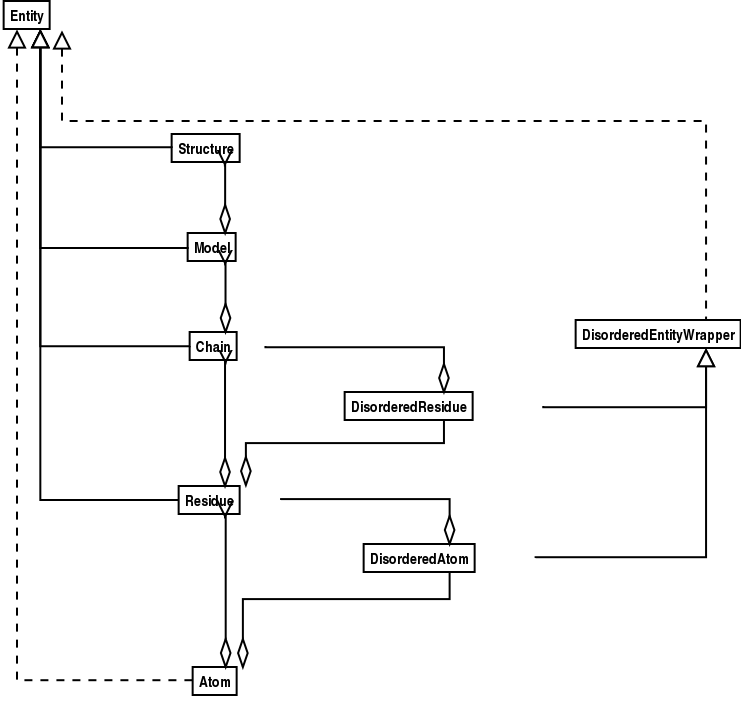
\includegraphics[width=0.8\textwidth]{images/smcra.png}
\caption{UML diagram of the SMCRA data structure
used to represent a macromolecular structure.}
\label{fig:smcra}
\end{figure}
\end{latexonly}

Structure, Model, Chain and Residue are all subclasses of the Entity base class.
The Atom class only (partly) implements the Entity interface (because an Atom
does not have children).

For each Entity subclass, you can extract a child by using a unique id for that
child as a key (e.g. you can extract an Atom object from a Residue object by
using an atom name string as a key, you can extract a Chain object from a Model
object by using its chain identifier as a key).

Disordered atoms and residues are represented by DisorderedAtom and DisorderedResidue
classes, which are both subclasses of the DisorderedEntityWrapper base class.
They hide the complexity associated with disorder and behave exactly as Atom
and Residue objects.

In general, a child Entity object (i.e. Atom, Residue, Chain, Model) can be
extracted from its parent (i.e. Residue, Chain, Model, Structure, respectively)
by using an id as a key.

\begin{verbatim}
child_entity=parent_entity[child_id]
\end{verbatim}

You can also get a list of all child Entities of a parent Entity object. Note
that this list is sorted in a specific way (e.g. according to chain identifier
for Chain objects in a Model object).

\begin{verbatim}
child_list=parent_entity.get_list()
\end{verbatim}

You can also get the parent from a child.

\begin{verbatim}
parent_entity=child_entity.get_parent()
\end{verbatim}

At all levels of the SMCRA hierarchy, you can also extract a \emph{full id}.
The full id is a tuple containing all id's starting from the top object (Structure)
down to the current object. A full id for a Residue object e.g. is something
like:

\begin{verbatim}
full_id=residue.get_full_id()

print full_id

("1abc", 0, "A", ("", 10, "A"))
\end{verbatim}

This corresponds to:

\begin{itemize}
\item The Structure with id \char`\"{}1abc\char`\"{}
\item The Model with id 0
\item The Chain with id \char`\"{}A\char`\"{}
\item The Residue with id (\char`\"{} \char`\"{}, 10, \char`\"{}A\char`\"{}).
\end{itemize}
The Residue id indicates that the residue is not a hetero-residue (nor a water)
because it has a blanc hetero field, that its sequence identifier is 10 and
that its insertion code is \char`\"{}A\char`\"{}.

Some other useful methods:

\begin{verbatim}
# get the entity's id

entity.get_id()

# check if there is a child with a given id

entity.has_id(entity_id)

# get number of children

nr_children=len(entity)
\end{verbatim}

It is possible to delete, rename, add, etc. child entities from a parent entity,
but this does not include any sanity checks (e.g. it is possible to add two
residues with the same id to one chain). This really should be done via a nice
Decorator class that includes integrity checking, but you can take a look at
the code (Entity.py) if you want to use the raw interface.

\subsubsection{Structure}

The Structure object is at the top of the hierarchy. Its id is a user given
string. The Structure contains a number of Model children. Most crystal structures
(but not all) contain a single model, while NMR structures typically consist
of several models. Disorder in crystal structures of large parts of molecules
can also result in several models.

\paragraph{Constructing a Structure object}

A Structure object is produced by a PDBParser object:

\begin{verbatim}
from Bio.PDB.PDBParser import PDBParser

p=PDBParser(PERMISSIVE=1)

structure_id="1fat"

filename="pdb1fat.ent"

s=p.get_structure(structure_id, filename)
\end{verbatim}

The {\tt PERMISSIVE} flag indicates that a number of common problems (see \ref{problem structures})
associated with PDB files will be ignored (but note that some atoms and/or residues
will be missing). If the flag is not present a {\tt PDBConstructionException}
will be generated during the parse operation.

\paragraph{Header and trailer}

You can extract the header and trailer (simple lists of strings) of the PDB
file from the PDBParser object with the {\tt get\_header} and {\tt get\_trailer}
methods.

\subsubsection{Model}

The id of the Model object is an integer, which is derived from the position
of the model in the parsed file (they are automatically numbered starting from
0). The Model object stores a list of Chain children.

\paragraph{Example}

Get the first model from a Structure object.

\begin{verbatim}
first_model=structure[0]
\end{verbatim}

\subsubsection{Chain}

The id of a Chain object is derived from the chain identifier in the structure
file, and can be any string. Each Chain in a Model object has a unique id. The
Chain object stores a list of Residue children.

\paragraph{Example}

Get the Chain object with identifier {}``A{}'' from a Model object.

\begin{verbatim}
chain_A=model["A"]
\end{verbatim}

\subsubsection{Residue}

Unsurprisingly, a Residue object stores a set of Atom children. In addition,
it also contains a string that specifies the residue name (e.g. {}``ASN{}'')
and the segment identifier of the residue (well known to X-PLOR users, but not
used in the construction of the SMCRA data structure).

The id of a Residue object is composed of three parts: the hetero field (hetfield),
the sequence identifier (resseq) and the insertion code (icode).

The hetero field is a string : it is {}``W{}'' for waters, {}``H\_{}'' followed
by the residue name (e.g. {}``H\_FUC{}'') for other hetero residues and blank
for standard amino and nucleic acids. This scheme is adopted for reasons described
in section \ref{hetero probems}.

The second field in the Residue id is the sequence identifier, an integer describing
the position of the residue in the chain.

The third field is a string, consisting of the insertion code. The insertion
code is sometimes used to preserve a certain desirable residue numbering scheme.
A Ser 80 insertion mutant (inserted e.g. between a Thr 80 and an Asn 81 residue)
could e.g. have sequence identifiers and insertion codes as followed: Thr 80
A, Ser 80 B, Asn 81. In this way the residue numbering scheme stays in tune
with that of the wild type structure.

Let's give some examples. Asn 10 with a blank insertion code would have residue
id {\tt ('' '', 10, '' '')}. Water 10 would have residue id {\tt (``W``, 10, `` ``)}.
A glucose molecule (a hetero residue with residue name GLC) with sequence identifier
10 would have residue id {\tt (''H\_GLC'', 10, '' '')}. In this way, the three
residues (with the same insertion code and sequence identifier) can be part
of the same chain because their residue id's are distinct.

In most cases, the hetflag and insertion code fields will be blank, e.g. {\tt ('' '', 10, '' '')}.
In these cases, the sequence identifier can be used as a shortcut for the full
id:

\begin{verbatim}
# use full id

res10=chain[("", 10, "")]

# use shortcut

res10=chain[10]
\end{verbatim}

Each Residue object in a Chain object should have a unique id. However, disordered
residues are dealt with in a special way, as described in section \ref{point mutations}.

A Residue object has a number of additional methods:

\begin{verbatim}
r.get_resname()		# return residue name, e.g. "ASN"
r.get_segid()		# return the SEGID, e.g. "CHN1"
\end{verbatim}

\subsubsection{Atom}

The Atom object stores the data associated with an atom, and has no children.
The id of an atom is its atom name (e.g. {}``OG{}'' for the side chain oxygen
of a Ser residue). An Atom id needs to be unique in a Residue. Again, an exception
is made for disordered atoms, as described in section \ref{disordered atoms}.

In a PDB file, an atom name consists of 4 chars, typically with leading and
trailing spaces. Often these spaces can be removed for ease of use (e.g. an
amino acid C\( \alpha  \) atom is labeled {}``.CA.{}'' in a PDB file, where
the dots represent spaces). To generate an atom name (and thus an atom id) the
spaces are removed, unless this would result in a name collision in a Residue
(i.e. two Atom objects with the same atom name and id). In the latter case,
the atom name including spaces is tried. This situation can e.g. happen when
one residue contains atoms with names {}``.CA.{}'' and {}``CA..{}'', although
this is not very likely.

The atomic data stored includes the atom name, the atomic coordinates (including
standard deviation if present), the B factor (including anisotropic B factors
and standard deviation if present), the altloc specifier and the full atom name
including spaces. Less used items like the atom element number or the atomic
charge sometimes specified in a PDB file are not stored.

An Atom object has the following additional methods:

\begin{verbatim}
a.get_name()       # atom name (spaces stripped, e.g. "CA")
a.get_id()         # id (equals atom name)
a.get_coord()      # atomic coordinates
a.get_bfactor()    # B factor
a.get_occupancy()  # occupancy
a.get_altloc()     # alternative location specifie
a.get_sigatm()     # std. dev. of atomic parameters
a.get_siguij()     # std. dev. of anisotropic B factor
a.get_anisou()     # anisotropic B factor
a.get_fullname()   # atom name (with spaces, e.g. ".CA.")
\end{verbatim}

To represent the atom coordinates, siguij, anisotropic B factor and sigatm Numpy
arrays are used.

\subsection{Disorder}

\subsubsection{General approach\label{disorder problems}}

Disorder should be dealt with from two points of view: the atom and the residue
points of view. In general, we have tried to encapsulate all the complexity that
arises from disorder. If you just want to loop over all C\( \alpha  \) atoms,
you do not care that some residues have a disordered side chain. On the other
hand it should also be possible to represent disorder completely in the data
structure. Therefore, disordered atoms or residues are stored in special objects
that behave as if there is no disorder. This is done by only representing a
subset of the disordered atoms or residues. Which subset is picked (e.g. which
of the two disordered OG side chain atom positions of a Ser residue is used)
can be specified by the user.

\subsubsection{Disordered atoms\label{disordered atoms}}

Disordered atoms are represented by ordinary Atom objects, but all Atom objects
that represent the same physical atom are stored in a DisorderedAtom object.
Each Atom object in a DisorderedAtom object can be uniquely indexed using its
altloc specifier. The DisorderedAtom object forwards all uncaught method calls
to the selected Atom object, by default the one that represents the atom with
with the highest occupancy. The user can of course change the selected Atom
object, making use of its altloc specifier. In this way atom disorder is represented
correctly without much additional complexity. In other words, if you are not
interested in atom disorder, you will not be bothered by it.

Each disordered atom has a characteristic altloc identifier. You can specify
that a DisorderedAtom object should behave like the Atom object associated with
a specific altloc identifier:

\begin{verbatim}
atom.disordered\_select("A")		# select altloc A atom

print atom.get_altloc()
"A"

atom.disordered_select("B")	   	# select altloc B atom
print atom.get_altloc()
"B"
\end{verbatim}

\subsubsection{Disordered residues}

\paragraph{Common case}

The most common case is a residue that contains one or more disordered atoms.
This is evidently solved by using DisorderedAtom objects to represent the disordered
atoms, and storing the DisorderedAtom object in a Residue object just like ordinary
Atom objects. The DisorderedAtom will behave exactly like an ordinary atom (in
fact the atom with the highest occupancy) by forwarding all uncaught method
calls to one of the Atom objects (the selected Atom object) it contains.

\paragraph{Point mutations\label{point mutations}}

A special case arises when disorder is due to a point mutation, i.e. when two
or more point mutants of a polypeptide are present in the crystal. An example
of this can be found in PDB structure 1EN2.

Since these residues belong to a different residue type (e.g. let's say Ser
60 and Cys 60) they should not be stored in a single Residue object as in the
common case. In this case, each residue is represented by one Residue object,
and both Residue objects are stored in a DisorderedResidue object.

The DisorderedResidue object forwards all uncaught methods to the selected Residue
object (by default the last Residue object added), and thus behaves like an
ordinary residue. Each Residue object in a DisorderedResidue object can be uniquely
identified by its residue name. In the above example, residue Ser 60 would have
id {}``SER{}'' in the DisorderedResidue object, while residue Cys 60 would
have id {}``CYS{}''. The user can select the active Residue object in a DisorderedResidue
object via this id.

\subsection{Hetero residues}

\subsubsection{Associated problems\label{hetero probems}}

A common problem with hetero residues is that several hetero and non-hetero
residues present in the same chain share the same sequence identifier (and insertion
code). Therefore, to generate a unique id for each hetero residue, waters and
other hetero residues are treated in a different way.

Remember that Residue object have the tuple (hetfield, resseq, icode) as id.
The hetfield is blank ({}`` {}``) for amino and nucleic acids, and a string
for waters and other hetero residues. The content of the hetfield is explained
below.

\subsubsection{Water residues}

The hetfield string of a water residue consists of the letter {}``W{}''. So
a typical residue id for a water is ({}``W{}'', 1, {}`` {}``).

\subsubsection{Other hetero residues}

The hetfield string for other hetero residues starts with {}``H\_{}'' followed
by the residue name. A glucose molecule e.g. with residue name {}``GLC{}''
would have hetfield {}``H\_GLC{}''. It's residue id could e.g. be ({}``H\_GLC{}'',
1, {}`` {}``).

\subsection{Some random usage examples}

Parse a PDB file, and extract some Model, Chain, Residue and Atom objects.

\begin{verbatim}
from Bio.PDB.PDBParser import PDBParser

parser=PDBParser()

structure=parser.get_structure("test", "1fat.pdb")
model=structure[0]
chain=model["A"]
residue=chain[1]
atom=residue["CA"]
\end{verbatim}

Extract a hetero residue from a chain (e.g. a glucose (GLC) moiety with resseq
10).

\begin{verbatim}
residue_id=("H_GLC", 10, " ")
residue=chain[residue_id]
\end{verbatim}

Print all hetero residues in chain.

\begin{verbatim}
for residue in chain.get_list():
	residue_id=residue.get_id()
	hetfield=residue_id[0]
	if hetfield[0]=="H":
		print residue_id
\end{verbatim}

Print out the coordinates of all CA atoms in a structure with B factor greater
than 50.

\begin{verbatim}
for model in structure.get_list():
  for chain in model.get_list():
    for residue in chain.get_list():
      if residue.has_id("CA"):
        ca=residue["CA"]
        if ca.get_bfactor()>50.0:
          print ca.get_coord()
\end{verbatim}

Print out all the residues that contain disordered atoms.

\begin{verbatim}
for model in structure.get_list():
  for chain in model.get_list():
    for residue in chain.get_list():
      if residue.is_disordered():
        resseq=residue.get_id()[1]
        resname=residue.get_resname()
        model_id=model.get_id()
        chain_id=chain.get_id()
        print model_id, chain_id, resname, resseq
\end{verbatim}

Loop over all disordered atoms, and select all atoms with altloc A (if present).
This will make sure that the SMCRA data structure will behave as if only the
atoms with altloc A are present.

\begin{verbatim}
for model in structure.get_list():
  for chain in model.get_list():
    for residue in chain.get_list():
      if residue.is_disordered():
        for atom in residue.get_list():
          if atom.is_disordered():
            if atom.disordered_has_id("A"):
              atom.disordered_select("A")
\end{verbatim}

Suppose that a chain has a point mutation at position 10, consisting of a Ser
and a Cys residue. Make sure that residue 10 of this chain behaves as the Cys
residue.

\begin{verbatim}
residue=chain[10]
residue.disordered_select("CYS")
\end{verbatim}

\subsection{Common problems in PDB files}

\subsubsection{Examples\label{problem structures}}

The PDBParser/Structure class was tested on about 800 structures (each belonging
to a unique SCOP superfamily). This takes about 20 minutes, or on average 1.5
seconds per structure. Parsing the structure of the large ribosomal subunit
(1FKK), which contains about 64000 atoms, takes 10 seconds on a 1000 MHz PC.

Three exceptions were generated in cases where an unambiguous data structure
could not be built. In all three cases, the likely cause is an error in the
PDB file that should be corrected. Generating an exception in these cases
is much better than running the chance of incorrectly describing
the structure in a data structure.

\paragraph{Duplicate residues}

One structure contains two amino acid residues in one chain with the same sequence
identifier (resseq 3) and icode. Upon inspection it was found that this chain
contains the residues Thr A3, \ldots{}, Gly A202, Leu A3, Glu A204. Clearly,
Leu A3 should be Leu A203. A couple of similar situations exist for structure
1FFK (which e.g. contains Gly B64, Met B65, Glu B65, Thr B67, i.e. residue Glu
B65 should be Glu B66).

\paragraph{Duplicate atoms}

Structure 1EJG contains a Ser/Pro point mutation in chain A at position 22.
In turn, Ser 22 contains some disordered atoms. As expected, all atoms belonging
to Ser 22 have a non-blank altloc specifier (B or C). All atoms of Pro 22 have
altloc A, except the N atom which has a blank altloc. This generates an exception,
because all atoms belonging to two residues at a point mutation should have
non-blank altloc. It turns out that this atom is probably shared by Ser and
Pro 22, as Ser 22 misses the N atom. Again, this points to a problem in the
file: the N atom should be present in both the Ser and the Pro residue, in both
cases associated with a suitable altloc identifier.

\subsubsection{Automatic correction}

Some errors are quite common and can be easily corrected without much risk of
making a wrong interpretation. These cases are listed below.

\paragraph{A blank altloc for a disordered atom}

Normally each disordered atom should have a non-blanc altloc identifier. However,
there are many structures that do not follow this convention, and have a blank
and a non-blank identifier for two disordered positions of the same atom. This
is automatically interpreted in the right way.

\paragraph{Broken chains}

Sometimes a structure contains a list of residues belonging to chain A, followed
by residues belonging to chain B, and again followed by residues belonging to
chain A, i.e. the chains are {}``broken{}''. This is correctly interpreted.

\subsubsection{Fatal errors}

Sometimes a PDB file cannot be unambiguously interpreted. Rather than guessing
and risking a mistake, an exception is generated, and the user is expected to
correct the PDB file. These cases are listed below.

\paragraph{Duplicate residues}

All residues in a chain should have a unique id. This id is generated based
on:

\begin{itemize}
\item The sequence identifier (resseq).
\item The insertion code (icode).
\item The hetfield string ({}``W{}'' for waters and {}``H\_{}'' followed by the
residue name for other hetero residues)
\item The residue names of the residues in the case of point mutations (to store the
Residue objects in a DisorderedResidue object).
\end{itemize}
If this does not lead to a unique id something is quite likely wrong, and an
exception is generated.

\paragraph{Duplicate atoms}

All atoms in a residue should have a unique id. This id is generated based on:

\begin{itemize}
\item The atom name (without spaces, or with spaces if a problem arises).
\item The altloc specifier.
\end{itemize}
If this does not lead to a unique id something is quite likely wrong, and an
exception is generated.

\subsection{Other features}

There are also some tools to analyze a crystal structure. Tools
exist to superimpose two coordinate sets (SVDSuperimposer), to extract
polypeptides from a structure (Polypeptide), to perform neighbor lookup
(NeighborSearch) and to write out PDB files (PDBIO). The neighbor lookup
is done using a KD tree module written in C++. It is very fast and also
includes a fast method to find all point pairs within a certain distance
of each other.

A Polypeptide object is simply a UserList of Residue objects. You can
construct a list of Polypeptide objects from a Structure object as follows:

\begin{verbatim}
model_nr=1
polypeptide_list=build_peptides(structure, model_nr)

for polypeptide in polypeptide_list:
    print polypeptide
\end{verbatim}

The Polypeptide objects are always created from a single
Model (in this case model 1).

\section{Bio.PopGen: Population genetics}

Bio.PopGen is a new Biopython module supporting population genetics,
available in Biopython 1.44 onwards.

The medium term objective for the module is to support widely used data
formats, applications and databases. This module is currently under intense
development and support for new features should appear at a rather fast pace.
Unfortunately this might also entail some instability on the API, especially
if you are using a CVS version. APIs that are made available on public
versions should be much stabler.

\subsection{GenePop}

GenePop (\url{http://genepop.curtin.edu.au/}) is a popular population
genetics software package supporting Hardy-Weinberg tests, linkage
desiquilibrium, population diferentiation, basic statistics, $F_{st}$ and
migration estimates, among others. GenePop does not supply sequence
based statistics as it doesn't handle sequence data.
The GenePop file format is supported by a wide range of other population
genetic software applications, thus making it a relevant format in the
population genetics field.

Bio.PopGen provides a parser and generator of GenePop file format.
Utilities to manipulate the content of a record are also provided.
Here is an example on how to read a GenePop file (you can find
example GenePop data files in the Test/PopGen directory of Biopython):

\begin{verbatim}
from Bio.PopGen import GenePop

handle = open("example.gen")
rec = GenePop.parse(handle)
handle.close()
\end{verbatim}

This will read a file called example.gen and parse it. If you
do print rec, the record will be output again, in GenePop format.

The most important information in rec will be the loci names and
population information (but there is more -- use help(GenePop.Record)
to check the API documentation). Loci names can be found on rec.loci\_list.
Population information can be found on rec.populations.
Populations is a list with one element per population. Each element is itself
a list of individuals, each individual is a pair composed by individual
name and a list of alleles (2 per marker), here is an example for
rec.populations:

\begin{verbatim}
[
    [
        ('Ind1', [(1, 2),    (3, 3), (200, 201)],
        ('Ind2', [(2, None), (3, 3), (None, None)],
    ],
    [
        ('Other1', [(1, 1),  (4, 3), (200, 200)],
    ]
]
\end{verbatim}

So we have two populations, the first with two individuals, the
second with only one. The first individual of the first
population is called Ind1, allelic information for each of
the 3 loci follows. Please note that for any locus, information
might be missing (see as an example, Ind2 above).

A few utility functions to manipulate GenePop records are made
available, here is an example:

\begin{verbatim}
from Bio.PopGen import GenePop

#Imagine that you have loaded rec, as per the code snippet above...

rec.remove_population(pos)
#Removes a population from a record, pos is the population position in
#  rec.populations, remember that it starts on position 0.
#  rec is altered.

rec.remove_locus_by_position(pos)
#Removes a locus by its position, pos is the locus position in
#  rec.loci_list, remember that it starts on position 0.
#  rec is altered.

rec.remove_locus_by_name(name)
#Removes a locus by its name, name is the locus name as in
#  rec.loci_list. If the name doesn't exist the function fails
#  silently.
#  rec is altered.

rec_loci = rec.split_in_loci()
#Splits a record in loci, that is, for each loci, it creates a new
#  record, with a single loci and all populations.
#  The result is returned in a dictionary, being each key the locus name.
#  The value is the GenePop record.
#  rec is not altered.

rec_pops =  rec.split_in_pops(pop_names)
#Splits a record in populations, that is, for each population, it creates
#  a new record, with a single population and all loci.
#  The result is returned in a dictionary, being each key
#  the population name. As population names are not available in GenePop,
#  they are passed in array (pop_names).
#  The value of each dictionary entry is the GenePop record.
#  rec is not altered.
\end{verbatim}

GenePop does not support population names, a limitation which can be
cumbersome at times. Functionality to enable population names is currently
being planned for Biopython. These extensions won't break compatibility in
any way with the standard format.  In the medium term, we would also like to
support the GenePop web service.

\subsection{Coalescent simulation}

A coalescent simulation is a backward model of population genetics with relation to
time. A simulation of ancestry is done until the Most Recent Common Ancestor (MRCA) is found.
This ancestry relationship starting on the MRCA and ending on the current generation
sample is sometimes called a genealogy. Simple cases assume a population of constant
size in time, haploidy, no population structure, and simulate the alleles of a single
locus under no selection pressure.

Coalescent theory is used in many fields like selection detection, estimation of
demographic parameters of real populations or disease gene mapping.

The strategy followed in the Biopython implementation of the coalescent was not
to create a new, built-in, simulator from scratch but to use an existing one,
SIMCOAL2 (\url{http://cmpg.unibe.ch/software/simcoal2/}). SIMCOAL2 allows for,
among others, population structure, multiple demographic events, simulation
of multiple types of loci (SNPs, sequences, STRs/microsatellites and RFLPs)
with recombination, diploidy multiple chromosomes or ascertainment bias. Notably
SIMCOAL2 doesn't support any selection model. We recommend reading SIMCOAL2's
documentation, available in the link above.

The input for SIMCOAL2 is a file specifying the desired demography and genome,
the output is a set of files (typically around 1000) with the simulated genomes
of a sample of individuals per subpopulation. This set of files can be used
in many ways, like to compute confidence intervals where which certain
statistics (e.g., $F_{st}$ or Tajima D) are expected to lie. Real population
genetics datasets statistics can then be compared to those confidence intervals.

Biopython coalescent code allows to create demographic scenarios and genomes and
to run SIMCOAL2.

\subsubsection{Creating scenarios}

Creating a scenario involves both creating a demography and a chromosome structure.
In many cases (e.g. when doing Approximate Bayesian Computations -- ABC) it is
important to test many parameter variations (e.g. vary the effective population size,
$N_e$, between 10, 50, 500 and 1000 individuals). The code provided allows for
the simulation of scenarios with different demographic parameters very easily.

Below we see how we can create scenarios and then how simulate them.

\paragraph{Demography}

A few predefined demographies are built-in, all have two shared parameters: sample size
(called sample\_size on the template, see below for its use) per deme and deme size, i.e.
subpopulation size (pop\_size). All demographies are available as templates where all
parameters can be varied, each template has a system name. The prefedined
demographies/templates are:

\begin{description}
\item[Single population, constant size] The standard parameters are enough to specifity
it. Template name: simple.
\item[Single population, bottleneck] As seen on figure \ref{fig:bottle}. The parameters
are current population size (pop\_size on template ne3 on figure), time of expansion,
given as the generation in the past when it occured (expand\_gen), 
effective population size during bottleneck (ne2), time of contraction
(contract\_gen) and original size in the remote past (ne3). Template name: bottle.
\item[Island model] The typical island model. The total number of demes is specified
by total\_demes and the migration rate by mig. Template name island.
\item[Stepping stone model - 1 dimension] The stepping stone model in 1 dimension,
extremes disconnected. The total number of demes is total\_demes, migration rate
is mig. Template name is ssm\_1d.
\item[Stepping stone model - 2 dimensions] The stepping stone model in 2 dimensions,
extremes disconnected. The parameters are x for the horizontal dimension and y
for the vertical (being the total number of demes x times y), migration rate is mig.
Template name is ssm\_2d.
\end{description}

\begin{htmlonly}
\label{fig:bottle}
\imgsrc{images/bottle.png}
\end{htmlonly}

\begin{latexonly}
\begin{figure}[htbp]
\centering
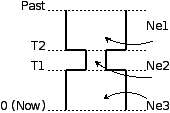
\includegraphics{images/bottle.png}
\caption{A bottleneck}
\label{fig:bottle}
\end{figure}
\end{latexonly}

In our first example, we will generate a template for a single population, constant size
model with a sample size of 30 and a deme size of 500. The code for this is:

\begin{verbatim}
from Bio.PopGen.SimCoal.Template import generate_simcoal_from_template

generate_simcoal_from_template('simple',
    [(1, [('SNP', [24, 0.0005, 0.0])])],
    [('sample_size', [30]),
    ('pop_size', [100])])
\end{verbatim}

Executing this code snippet will generate a file on the current directory called
simple\_100\_300.par this file can be given as input to SIMCOAL2 to simulate the
demography (below we will see how Biopython can take care of calling SIMCOAL2).

This code consists of a single function call, let's discuss it parameter by parameter.

The first parameter is the template id (from the list above). We are using the id
'simple' which is the template for a single population of constant size along time.

The second parameter is the chromosome structure. Please ignore it for now, it will be
explained in the next section.

The third parameter is a list of all required parameters (recall that the simple model
only needs sample\_size and pop\_size) and possible values (in this case each
parameter only has a possible value).

Now, let's consider an example where we want to generate several island models, and we
are interested in varying the number of demes: 10, 50 and 100 with a migration
rate of 1\%. Sample size and deme
size will be the same as before. Here is the code:


\begin{verbatim}
from Bio.PopGen.SimCoal.Template import generate_simcoal_from_template

generate_simcoal_from_template('island',
    [(1, [('SNP', [24, 0.0005, 0.0])])],
    [('sample_size', [30]),
    ('pop_size', [100]),
    ('mig', [0.01]),
    ('total_demes', [10, 50, 100])])
\end{verbatim}

In this case, 3 files will be generated: island\_100\_0.01\_100\_30.par,
island\_10\_0.01\_100\_30.par and island\_50\_0.01\_100\_30.par. Notice the
rule to make file names: template name, followed by parameter values in
reverse order.

A few, arguably more esoteric template demographies exist (please check the
Bio/PopGen/SimCoal/data directory on Biopython source tree). Furthermore it is possible
for the user to create new templates. That functionality will be discussed in a future
version of this document.

\paragraph{Chromosome structure}

We strongly recommend reading SIMCOAL2 documentation to understand the full potential
available in modeling chromosome structures. In this subsection we only discuss how
to implement chromosome structures using the Biopython interface, not the underlying
SIMCOAL2 capabilities.

We will start by implementing a single chromosome, with 24 SNPs with
a recombination rate immediately on the right of each locus of 0.0005 and a
minimum frequency of the minor allele of 0. This will be specified by the
following list (to be passed as second parameter to the function
generate\_simcoal\_from\_template):

\begin{verbatim}
[(1, [('SNP', [24, 0.0005, 0.0])])]
\end{verbatim}

This is actually the chromosome structure used in the above examples.


The chromosome structure is represented by a list of chromosomes,
each chromosome (i.e., each element in the list)
is composed by a tuple (a pair): the first element
is the number of times the chromosome is to be repeated (as there
might be interest in repeating the same chromosome many times).
The second element is a list of the actual components of the chromosome.
Each element is again a pair, the first member is the locus type and
the second element the parameters for that locus type. Confused?
Before showing more examples let's review the example above: We have
a list with one element (thus one chromosome), the chromosome is
a single instance (therefore not to be repeated), it is composed
of 24 SNPs, with a recombination rate of 0.0005 between each
consecutive SNP, the minimum frequency of the minor allele is
0.0 (i.e, it can be absent from a certain population).

Let's see a more complicated example:

\begin{verbatim}
[
  (5, [
       ('SNP', [24, 0.0005, 0.0])
      ]
  ),
  (2, [
       ('DNA', [10, 0.0, 0.00005, 0.33]),
       ('RFLP', [1, 0.0, 0.0001]),
       ('MICROSAT', [1, 0.0, 0.001, 0.0, 0.0])
      ]
  )
]
\end{verbatim}

We start by having 5 chromosomes with the same structure as
above (i.e., 24 SNPs). We then have 2 chromosomes which
have a DNA sequence with 10 nucleotides, 0.0 recombination rate,
0.0005 mutation rate, and a transition rate of 0.33. Then we
have an RFLP with 0.0 recombination rate to the next locus and
a 0.0001 mutation rate. Finally we have a microsatellite (or STR),
with 0.0 recombination rate to the next locus (note, that as this
is a single microsatellite which has no loci following, this
recombination rate here is irrelevant), with a mutation rate
of 0.001, geometric paramater of 0.0 and a range constraint
of 0.0 (for information about this parameters please consult
the SIMCOAL2 documentation, you can use them to simulate
various mutation models, including the typical  -- for microsatellites --
stepwise mutation model among others).


\subsubsection{Running SIMCOAL2}

We now discuss how to run SIMCOAL2 from inside Biopython. It is required
that the binary for SIMCOAL2 is called simcoal2 (or simcoal2.exe on Windows
based platforms), please note that the typical name when downloading the
program is in the format simcoal2\_x\_y. As such renaming of the binary
after download is needed.

It is possible to run SIMCOAL2 on files that were not generated using the method
above (e.g., writing a parameter file by hand), but we will show an
example by creating a model using the framework presented above.

\begin{verbatim}
from Bio.PopGen.SimCoal.Template import generate_simcoal_from_template
from Bio.PopGen.SimCoal.Controller import SimCoalController


generate_simcoal_from_template('simple',
    [
      (5, [
           ('SNP', [24, 0.0005, 0.0])
          ]
      ),
      (2, [
           ('DNA', [10, 0.0, 0.00005, 0.33]),
           ('RFLP', [1, 0.0, 0.0001]),
           ('MICROSAT', [1, 0.0, 0.001, 0.0, 0.0])
          ]
      )
    ],
    [('sample_size', [30]),
    ('pop_size', [100])])

ctrl = SimCoalController('.')
ctrl.run_simcoal('simple_100_30.par', 50)
\end{verbatim}

The lines of interest are the last two (plus the new import).
Firstly a controller for the
application is created. The directory where the binary is located has
to be specified.

The simulator is then run on the last line: we know, from the rules explained
above, that the input file name is simple\_100\_30.par for the
simulation parameter file created. We then specify
that we want to run 50 independent simulations, by default Biopython
requests a simulation of diploid data, but a third parameter can
be added to simulate haploid data (adding as a parameter the
string '0'). SIMCOAL2 will now run (please
note that this can take quite a lot of time) and will create a directory
with the simulation results. The results can now be analysed (typically
studying the data with Arlequin3). In the future Biopython might support
reading the Arlequin3 format and thus allowing for the analysis of SIMCOAL2
data inside Biopython.


\subsection{Other applications}

Here we discuss interfaces and utilities to deal with population genetics'
applications which arguably have a smaller user base.

\subsubsection{FDist: Detecting selection and molecular adaptation}

FDist is a selection detection application suite based on computing
(i.e. simulating) a ``neutral'' confidence interval based on $F_{st}$ and
heterozygosity. Markers (which can be SNPs, microsatellites, AFLPs
among others) which lie outside the ``neutral'' interval are to be
considered as possible candidates for being under selection.

FDist is mainly used when the number of markers is considered enough
to estimate an average $F_{st}$, but not enough to either have outliers
calculated from the dataset directly or, with even more markers for
which the relative positions in the genome are known, to use
approaches based on, e.g., Extended Haplotype Heterozygosity (EHH).

The typical usage pattern for FDist is as follows:

\begin{enumerate}
\item Import a dataset from an external format into FDist format.
\item Compute average $F_{st}$. This is done by datacal inside FDist.
\item Simulate ``neutral'' markers based on the
    average $F_{st}$ and expected number of total populations.
    This is the core operation, done by fdist inside FDist.
\item Calculate the confidence interval, based on the desired
    confidence boundaries (typically 95\% or 99\%). This is done by
    cplot and is mainly used to plot the interval.
\item Assess each marker status against the simulation ``neutral''
    confidence interval. Done
    by pv. This is used to detect the outlier status of each marker
    against the simulation.
\end{enumerate}

We will now discuss each step with illustrating example code
(for this example to work FDist binaries have to be on the
executable PATH).

The FDist data format is application specific and is not used at
all by other applications, as such you will probably have to convert
your data for use with FDist. Biopython can help you do this.
Here is an example converting from GenePop format to FDist format
(along with imports that will be needed on examples further below):

\begin{verbatim}
from Bio.PopGen import GenePop
from Bio.PopGen import FDist
from Bio.PopGen.FDist import Controller
from Bio.PopGen.FDist.Utils import convert_genepop_to_fdist

gp_rec = GenePop.parse(open("example.gen"))
fd_rec = convert_genepop_to_fdist(gp_rec)
in_file = open("infile", "w")
in_file.write(str(fd_rec))
in_file.close()
\end{verbatim}

In this code we simply parse a GenePop file and convert it to a FDist
record.

Printing an FDist record will generate
a string that can be directly saved to a file and supplied to FDist. FDist
requires the input file to be called infile, therefore we save the record on
a file with that name.

The most important fields on a FDist record are: num\_pops, the number of
populations; num\_loci, the number of loci and loci\_data with the marker
data itself. Most probably the details of the record are of no interest
to the user, as the record only purpose is to be passed to FDist.

The next step is to calculate the average $F_{st}$ of the dataset (along
with the sample size):

\begin{verbatim}
ctrl = Controller.FDistController()
fst, samp_size = ctrl.run_datacal()
\end{verbatim}

On the first line we create an object to control the call of  FDist
suite, this object will be used further on in order to call other
suite applications.

On the second line we call the datacal application which computes the
average $F_{st}$
and the sample size. It is worth noting that the $F_{st}$ computed by
datacal is a \emph{variation} of Weir and Cockerham's $\theta$.

We can now call the main fdist application in order to simulate neutral
markers.

\begin{verbatim}
sim_fst = ctrl.run_fdist(npops = 15, nsamples = fd_rec.num_pops, fst = fst,
    sample_size = samp_size, mut = 0, num_sims = 40000)
\end{verbatim}

\begin{description}
\item[npops] Number of populations existing in nature. This is really a
    ``guestimate''. Has to be lower than 100.
\item[nsamples] Number of populations sampled, has to be lower than npops.
\item[fst] Average $F_{st}$.
\item[sample\_size] Average number of individuals sampled on each population.
\item[mut] Mutation model: 0 - Infinite alleles; 1 - Stepwise mutations
\item[num\_sims] Number of simulations to perform. Typically a number around
    40000 will be OK, but if you get a confidence interval that looks sharp
    (this can be detected when plotting the confidence interval computed
    below) the value can be increased (a suggestion would be steps of 10000
    simulations).
\end{description}

The confusion in wording between number of samples and sample size
stems from the original application.

A file named out.dat will be created with the simulated heterozygosities
and $F_{st}$s, it will have as many lines as the number of simulations
requested.

Note that fdist returns the average $F_{st}$ that it was \emph{capable} of
simulating, for more details about this issue please read below the paragraph
on approximating the desired average $F_{st}$.

The next (optional) step is to calculate the confidence interval:

\begin{verbatim}
cpl_interval = ctrl.run_cplot(ci=0.99)
\end{verbatim}

You can only call cplot after having run fdist.

This will calculate the confidence intervals (99\% in this case)
for a previous fdist run. A list of quadruples is returned. The
first element represents the heterozygosity, the second the lower
bound of $F_{st}$ confidence interval for that heterozygosity,
the third the average and the fourth the upper bound. This can
be used to trace the confidence interval contour. This list
is also written to a file, out.cpl.

The main purpose of this step is return a set of points which can
be easily used to plot a confidence interval. It can be skipped
if the objective is only to assess the status of each marker against
the simulation, which is the next step...

\begin{verbatim}
pv_data = ctrl.run_pv()
\end{verbatim}

You can only call cplot after having run datacal and fdist.

This will use the simulated markers to assess the status of each
individual real marker. A list, in the same order than the loci\_list
that is on the FDist record (which is in the same order that the GenePop
record) is returned. Each element in the list is a quadruple, the
fundamental member of each quadruple is the last element (regarding the
other elements, please refer to the pv documentation -- for the
sake of simplicity we will not discuss them here) which returns the
probability of the simulated $F_{st}$ being lower than the marker $F_{st}$.
Higher values would indicate a stronger candidate for positive selection,
lower values a candidate for balancing selection, and intermediate values
a possible neutral marker. What is ``higher'', ``lower'' or ``intermediate''
is really a subjective issue, but taking a ``confidence interval'' approach
and considering a 95\% confidence interval, ``higher'' would be between 0.95
and 1.0, ``lower'' between 0.0 and 0.05 and ``intermediate'' between 0.05 and
0.95.

\paragraph{Approximating the desired average $F_{st}$}

Fdist tries to approximate the desired average $F_{st}$ by doing a
coalescent simulation using migration rates based on the formula

\[ N_{m} = \frac{1 - F_{st}}{4F_{st}} \]

This formula assumes a few premises like an infinite number of populations.

In practice, when the number of populations is low, the mutation model
is stepwise and the sample size increases, fdist will not be able to
simulate an acceptable approximate average $F_{st}$.

To address that, a function is provided to iteratively approach the desired
value by running several fdists in sequence. This approach is computationally
more intensive than running a single fdist run, but yields good results.
The following code runs fdist approximating the desired $F_{st}$:

\begin{verbatim}
sim_fst = ctrl.run_fdist_force_fst(npops = 15, nsamples = fd_rec.num_pops,
    fst = fst, sample_size = samp_size, mut = 0, num_sims = 40000,
    limit = 0.05)
\end{verbatim}

The only new optional parameter, when comparing with run\_fdist, is limit
which is the desired maximum error. run\_fdist can (and probably should)
be safely replaced with run\_fdist\_force\_fst.

\paragraph{Final notes}

The process to determine the average $F_{st}$ can be more sophisticated than
the one presented here. For more information we refer you to the FDist
README file. Biopython's code can be used to implement more sophisticated
approaches.

\subsection{Future Developments}

The most desired future developments would be the ones you add yourself ;) .

That being said, already existing fully functional code is currently being
incorporated in Bio.PopGen, that code covers the applications FDist and
SimCoal2, the HapMap and UCSC Table Browser databases and some simple statistics
like $F_{st}$, or allele counts.

\section{InterPro}

The \verb|Bio.InterPro| module works with files from the
InterPro database, which can be obtained from the InterPro project:
\url{http://www.ebi.ac.uk/interpro/}.

The \verb|Bio.InterPro.Record| contains all the information stored in
an InterPro record. Its string representation also is a valid InterPro
record, but it is NOT guaranteed to be equivalent to the record
from which it was produced.

The \verb|Bio.InterPro.Record| contains:

\begin{itemize}
  \item \verb|Database|
  \item \verb|Accession|
  \item \verb|Name|
  \item \verb|Dates|
  \item \verb|Type|
  \item \verb|Parent|
  \item \verb|Process|
  \item \verb|Function|
  \item \verb|Component|
  \item \verb|Signatures|
  \item \verb|Abstract|
  \item \verb|Examples|
  \item \verb|References|
  \item \verb|Database links|
\end{itemize}

\chapter{Advanced}
\label{chapter:advanced}

\section{The SeqRecord and SeqFeature classes}
\label{sec:advanced-seq}

You read all about the basic Biopython sequence class in Chapter~\ref{chapter:Bio.Seq}, which described how to do many useful things with just the sequence. However, many times sequences have important additional properties associated with them -- as you will have seen with the \verb|SeqRecord| object in Chapter~\ref{chapter:Bio.SeqIO}.
This section describes how Biopython handles these higher level descriptions of a sequence.

\subsection{Sequence IDs and Descriptions -- dealing with SeqRecords}

Immediately above the Sequence class is the Sequence Record class, defined in the \verb|Bio.SeqRecord| module. This class allows higher level features such as ids and features to be associated with the sequence, and is used thoughout the sequence input/output interface \verb|Bio.SeqIO|, described in Chapter~\ref{chapter:Bio.SeqIO}. The \verb|SeqRecord|class itself is very simple, and offers the following information as attributes:

\begin{description}
  \item[seq] -- The sequence itself -- A \verb|Seq| object

  \item[id] -- The primary ID used to identify the sequence -- a string. In most cases this is something like an accession number.

  \item[name] -- A ``common'' name/id for the sequence -- a string. In some cases this will be the same as the accession number, but it could also be a clone name. I think of this as being analagous to the LOCUS id in a GenBank record.

  \item[description] -- A human readible description or expressive name for the sequence -- as string. This is similar to what follows the id information in a FASTA formatted entry.

  \item[annotations] -- A dictionary of additional information about the sequence. The keys are the name of the information, and the information is contained in the value. This allows the addition of more ``unstructed'' information to the sequence.

  \item[features] -- A list of \verb|SeqFeature| objects with more structured information about the features on a sequence. The structure of sequence features is described below in Section~\ref{sec:seq_features}.
  
  \item[dbxrefs] - A list of database cross-references as strings.
\end{description}

Using a \verb|SeqRecord| class is not very complicated, since all of the information is stored as attributes of the class. Initializing the class just involves passing a \verb|Seq| object to the \verb|SeqRecord|:

\begin{verbatim}
>>> from Bio.Seq import Seq
>>> simple_seq = Seq("GATC")
>>> from Bio.SeqRecord import SeqRecord
>>> simple_seq_r = SeqRecord(simple_seq)
\end{verbatim}

Additionally, you can also pass the id, name and description to the initialization function, but if not they will be set as strings indicating they are unknown, and can be modified subsequently:

\begin{verbatim}
>>> simple_seq_r.id
'<unknown id>'
>>> simple_seq_r.id = 'AC12345'
>>> simple_seq_r.description = 'My little made up sequence I wish I could
write a paper about and submit to GenBank'
>>> print simple_seq_r.description
My little made up sequence I wish I could write a paper about and submit
to GenBank
>>> simple_seq_r.seq
Seq('GATC', Alphabet())
\end{verbatim}

Adding annotations is almost as easy, and just involves dealing directly with the annotation dictionary:

\begin{verbatim}
>>> simple_seq_r.annotations['evidence'] = 'None. I just made it up.'
>>> print simple_seq_r.annotations
{'evidence': 'None. I just made it up.'}
\end{verbatim}

That's just about all there is to it! Next, you may want to learn about SeqFeatures, which offer an additional structured way to represent information about a sequence.

\subsection{Features and Annotations -- SeqFeatures}
\label{sec:seq_features}

Sequence features are an essential part of describing a sequence. Once you get beyond the sequence itself, you need some way to organize and easily get at the more ``abstract'' information that is known about the sequence. While it is probably impossible to develop a general sequence feature class that will cover everything, the Biopython \verb|SeqFeature| class attempts to encapsulate as much of the information about the sequence as possible. The design is heavily based on the GenBank/EMBL feature tables, so if you understand how they look, you'll probably have an easier time grasping the structure of the Biopython classes.

\subsubsection{SeqFeatures themselves}

The first level of dealing with sequence features is the \verb|SeqFeature| class itself. This class has a number of attributes, so first we'll list them and there general features, and then work through an example to show how this applies to a real life example, a GenBank feature table. The attributes of a SeqFeature are:

\begin{description}
  \item[location] -- The location of the \verb|SeqFeature| on the sequence that you are dealing with. The locations end-points may be fuzzy -- section~\ref{sec:locations} has a lot more description on how to deal with descriptions.

  \item[type] -- This is a textual description of the type of feature (for instance, this will be something like 'CDS' or 'gene').

  \item[ref] -- A reference to a different sequence. Some times features may be ``on'' a particular sequence, but may need to refer to a different sequence, and this provides the reference (normally an accession number). A good example of this is a genomic sequence that has most of a coding sequence, but one of the exons is on a different accession. In this case, the feature would need to refer to this different accession for this missing exon.

  \item[ref\_db] -- This works along with \verb|ref| to provide a cross sequence reference. If there is a reference, \verb|ref_db| will be set as None if the reference is in the same database, and will be set to the name of the database otherwise.

  \item[strand] -- The strand on the sequence that the feature is located on. This may either be '1' for the top strand, '-1' for the bottom strand, or '0' for both strands (or if it doesn't matter). Keep in mind that this only really makes sense for double stranded DNA, and not for proteins or RNA.

  \item[qualifiers] -- This is a python dictionary of additional information about the feature. The key is some kind of terse one-word description of what the information contained in the value is about, and the value is the actual information. For example, a common key for a qualifier might be ``evidence'' and the value might be ``computational (non-experimental).'' This is just a way to let the person who is looking at the feature know that it has not be experimentally (i.~e.~in a wet lab) confirmed.
 

  \item[sub\_features] -- A very important feature of a feature is that it can have additional \verb|sub_features| underneath it. This allows nesting of features, and helps us to deal with things such as the GenBank/EMBL feature lines in a (we hope) intuitive way.
\end{description}

To show an example of SeqFeatures in action, let's take a look at the following feature from a GenBank feature table:

\begin{verbatim}
     mRNA            complement(join(<49223..49300,49780..>50208))
                     /gene="F28B23.12"
\end{verbatim}

To look at the easiest attributes of the SeqFeature first, if you got a SeqFeature object for this it would have it \verb|type| of 'mRNA', a \verb|strand| of -1 (due to the 'complement'), and would have None for the \verb|ref| and \verb|ref_db| since there are no references to external databases. The \verb|qualifiers| for this SeqFeature would be a python dictionarary that looked like \verb|{'gene' : 'F28B23.12'}|.

Now let's look at the more tricky part, how the 'join' in the location
line is handled. First, the location for the top level SeqFeature (the
one we are dealing with right now) is set as going from
\verb|'<49223' to '>50208'| (see section~\ref{sec:locations} for
the nitty gritty on how fuzzy locations like this are handled).
So the location of the top level object is the entire span of the
feature. So, how do you get at the information in the 'join?'
Well, that's where the \verb|sub_features| go in.

The \verb|sub_features| attribute will have a list with two SeqFeature
objects in it, and these contain the information in the join. Let's
look at \verb|top_level_feature.sub_features[0]|; the first
\verb|sub_feature|). This object is a SeqFeature object with a
\verb|type| of '\verb|mRNA_join|,' a \verb|strand| of -1 (inherited
from the parent SeqFeature) and a location going from
\verb|'<49223' to '49300'|.

So, the \verb|sub_features| allow you to get at the internal information if you want it (i.~e.~if you were trying to get only the exons out of a genomic sequence), or just to deal with the broad picture (i.~e.~you just want to know that the coding sequence for a gene lies in a region). Hopefully this structuring makes it easy and intuitive to get at the sometimes complex information that can be contained in a SeqFeature.

\subsubsection{Locations}
\label{sec:locations}

In the section on SeqFeatures above, we skipped over one of the more difficult parts of Features, dealing with the locations. The reason this can be difficult is because of fuzziness of the positions in locations. Before we get into all of this, let's just define the vocabulary we'll use to talk about this. Basically there are two terms we'll use:

\begin{description}
  \item[position] -- This refers to a single position on a sequence,
  which may be fuzzy or not. For instance, 5, 20, \verb|<100| and
  \verb|3^5| are all positions.

  \item[location] -- A location is two positions that defines a region of a sequence. For instance 5..20 (i.~e.~5 to 20) is a location.
\end{description}

I just mention this because sometimes I get confused between the two.

The complication in dealing with locations comes in the positions themselves. In biology many times things aren't entirely certain (as much as us wet lab biologists try to make them certain!). For instance, you might do a dinucleotide priming experiment and discover that the start of mRNA transcript starts at one of two sites. This is very useful information, but the complication comes in how to represent this as a position. To help us deal with this, we have the concept of fuzzy positions. Basically there are five types of fuzzy positions, so we have five classes do deal with them:

\begin{description}
  \item[ExactPosition] -- As its name suggests, this class represents a position which is specified as exact along the sequence. This is represented as just a a number, and you can get the position by looking at the \verb|position| attribute of the object.

  \item[BeforePosition] -- This class represents a fuzzy position
  that occurs prior to some specified site. In GenBank/EMBL notation,
  this is represented as something like \verb|'<13'|, signifying that
  the real position is located somewhere less then 13. To get
  the specified upper boundary, look at the \verb|position|
  attribute of the object.

  \item[AfterPosition] -- Contrary to \verb|BeforePosition|, this
  class represents a position that occurs after some specified site.
  This is represented in GenBank as \verb|'>13'|, and like
  \verb|BeforePosition|, you get the boundary number by looking
  at the \verb|position| attribute of the object.

  \item[WithinPosition] -- This class models a position which occurs somewhere between two specified nucleotides. In GenBank/EMBL notation, this would be represented as '(1.5)', to represent that the position is somewhere within the range 1 to 5. To get the information in this class you have to look at two attributes. The \verb|position| attribute specifies the lower boundary of the range we are looking at, so in our example case this would be one. The \verb|extension| attribute specifies the range to the higher boundary, so in this case it would be 4. So \verb|object.position| is the lower boundary and \verb|object.position + object.extension| is the upper boundary.

  \item[BetweenPosition] -- This class deals with a position that
  occurs between two coordinates. For instance, you might have a
  protein binding site that occurs between two nucleotides on a
  sequence. This is represented as \verb|'2^3'|, which indicates that
  the real position happens between position 2 and 3. Getting
  this information from the object is very similar to
  \verb|WithinPosition|, the \verb|position| attribute specifies
  the lower boundary (2, in this case) and the \verb|extension|
  indicates the range to the higher boundary (1 in this case).
\end{description}

Now that we've got all of the types of fuzzy positions we can have taken care of, we are ready to actually specify a location on a sequence. This is handled by the \verb|FeatureLocation| class. An object of this type basically just holds the potentially fuzzy start and end positions of a feature. You can create a \verb|FeatureLocation| object by creating the positions and passing them in:

\begin{verbatim}
>>> from Bio import SeqFeature
>>> start_pos = SeqFeature.AfterPosition(5)
>>> end_pos = SeqFeature.BetweenPosition(8, 1)
>>> my_location = SeqFeature.FeatureLocation(start_pos, end_pos)
\end{verbatim}

If you print out a \verb|FeatureLocation| object, you can get a nice representation of the information:

\begin{verbatim}
>>> print my_location
[>5:(8^9)]
\end{verbatim}

We can access the fuzzy start and end positions using the start and end attributes of the location:

\begin{verbatim}
>>> my_location.start
<Bio.SeqFeature.AfterPosition instance at 0x101d7164>
>>> print my_location.start
>5
>>> print my_location.end
(8^9)
\end{verbatim}

If you don't want to deal with fuzzy positions and just want numbers, you just need to ask for the \verb|nofuzzy_start| and \verb|nofuzzy_end| attributes of the location:

\begin{verbatim}
>>> my_location.nofuzzy_start
5
>>> my_location.nofuzzy_end
8
\end{verbatim}

Notice that this just gives you back the position attributes of the fuzzy locations.

Similary, to make it easy to create a position without worrying about fuzzy positions, you can just pass in numbers to the \verb|FeaturePosition| constructors, and you'll get back out \verb|ExactPosition| objects:

\begin{verbatim}
>>> exact_location = SeqFeature.FeatureLocation(5, 8)
>>> print exact_location
[5:8]
>>> exact_location.start
<Bio.SeqFeature.ExactPosition instance at 0x101dcab4>
\end{verbatim}

That is all of the nitty gritty about dealing with fuzzy positions in Biopython. It has been designed so that dealing with fuzziness is not that much more complicated than dealing with exact positions, and hopefully you find that true!

\subsubsection{References}

Another common annotation related to a sequence is a reference to a journal or other published work dealing with the sequence. We have a fairly simple way of representing a Reference in Biopython -- we have a \verb|Bio.SeqFeature.Reference| class that stores the relevant information about a reference as attributes of an object.

The attributes include things that you would expect to see in a reference like \verb|journal|, \verb|title| and \verb|authors|. Additionally, it also can hold the \verb|medline_id| and \verb|pubmed_id| and a \verb|comment| about the reference. These are all accessed simply as attributes of the object.

A reference also has a \verb|location| object so that it can specify a particular location on the sequence that the reference refers to. For instance, you might have a journal that is dealing with a particular gene located on a BAC, and want to specify that it only refers to this position exactly. The \verb|location| is a potentially fuzzy location, as described in section~\ref{sec:locations}.

That's all there is too it. References are meant to be easy to deal with, and hopefully general enough to cover lots of usage cases.

\section{Regression Testing Framework}
\label{sec:regr_test}

Biopython has a regression testing framework originally written by Andrew Dalke and ported to PyUnit by Brad Chapman which helps us make sure the code is as bug-free as possible before going out.

\subsection{Writing a Regression Test}

Every module that goes into Biopython should have a test (and should also have documentation!). Let's say you've written a new module called Biospam -- here is what you should do to make a regression test:

\begin{enumerate}
  \item Write a script called \verb|test_Biospam.py|

  \begin{itemize}

    \item This script should live in the Tests directory
      
     \item The script should test all of the important functionality of the module (the more you test the better your test is, of course!).
    
     \item Try to avoid anything which might be platform specific, such as printing floating point numbers without using an explicit formatting string.
  \end{itemize}
      
  \item If the script requires files to do the testing, these should go in
       the directory Tests/Biospam.
      
  \item Write out the test output and verify the output to be correct.
       There are two ways to do this:

  \begin{enumerate}
    \item The long way:

    \begin{itemize}
      
     \item Run the script and write its output to a file. On UNIX machines,
       you would do something like: \verb|python test_Biospam.py > test_Biospam| which would write the output to the file \verb|test_Biospam|.
      
     \item Manually look at the file \verb|test_Biospam| to make sure the output is correct. When you are sure it is all right and there are no bugs, you need to quickly edit the \verb|test_Biospam| file so that the first line is: `\verb|test_Biospam|' (no quotes).

     \item copy the \verb|test_Biospam| file to the directory Tests/output
    
   \end{itemize}

   \item The quick way:

   \begin{itemize}
      \item Run \verb|python run_tests.py -g test_Biospam.py|. The
            regression testing framework is nifty enough that it'll put
            the output in the right place in just the way it likes it.  
      
       \item Go to the output (which should be in \verb|Tests/output/test_Biospam|) and double check the output to make sure it is all correct.

   \end{itemize}

 \end{enumerate}
      
 \item Now change to the Tests directory and run the regression tests
       with \verb|python run_tests.py|. This will run all of the tests, and
       you should see your test run (and pass!).
      
  \item That's it! Now you've got a nice test for your module ready to check into CVS.
       Congratulations!
\end{enumerate}

\section{Parser Design}

Many of the older Biopython parsers were built around an event-oriented
design that includes Scanner and Consumer objects.

Scanners take input from a data source and analyze it line by line,
sending off an event whenever it recognizes some information in the
data.  For example, if the data includes information about an organism
name, the scanner may generate an \verb|organism_name| event whenever it
encounters a line containing the name.

Consumers are objects that receive the events generated by Scanners.
Following the previous example, the consumer receives the
\verb|organism_name| event, and the processes it in whatever manner
necessary in the current application.

This is a very flexible framework, which is advantageous if you want to
be able to parse a file format into more than one representation.  For
example, both the \verb|Bio.GenBank| and \verb|Bio.SwissProt| modules
use this to read their file formats as both generic \verb|SeqRecord| objects
and file-format-specific record objects.

More recently, many of the parsers added for \verb|Bio.SeqIO| and
\verb|Bio.AlignIO| take a much simpler approach, but only generate a
single object representation (\verb|SeqRecord| and \verb|Alignment| objects
respectively).

\section{Substitution Matrices}

\subsection{SubsMat}

This module provides a class and a few routines for generating substitution matrices, similar to BLOSUM or PAM matrices, but based on user-provided data.

Additionally, you may select a matrix from MatrixInfo.py, a collection of established substitution matrices.

\begin{verbatim}
class SeqMat(UserDict.UserDict)
\end{verbatim}

\begin{enumerate}
  \item Attributes

  \begin{enumerate}
    \item \verb|self.data|: a dictionary in the form of \verb|{(i1,j1):n1, (i1,j2):n2,...,(ik,jk):nk}| where i, j are alphabet letters, and n is a value.

    \item \verb|self.alphabet|: a class as defined in Bio.Alphabet

    \item \verb|self.ab_list|: a list of the alphabet's letters, sorted. Needed mainly for internal purposes

    \item \verb|self.sum_letters|: a dictionary. \verb|{i1: s1, i2: s2,...,in:sn}| where:
    \begin{enumerate}
      \item i: an alphabet letter;
      \item s: sum of all values in a half-matrix for that letter;
      \item n: number of letters in alphabet.
    \end{enumerate}
  \end{enumerate}

  \item Methods

  \begin{enumerate}

    \item
\begin{verbatim}
__init__(self,data=None,alphabet=None,
         mat_type=NOTYPE,mat_name='',build_later=0):
\end{verbatim}

    \begin{enumerate}

      \item \verb|data|: can be either a dictionary, or another SeqMat instance.
      \item \verb|alphabet|: a Bio.Alphabet instance. If not provided, construct an alphabet from data.

      \item \verb|mat_type|: type of matrix generated. One of the following:

      \begin{description}
        \item[NOTYPE]     No type defined
        \item[ACCREP]     Accepted Replacements Matrix
        \item[OBSFREQ]    Observed Frequency Matrix
        \item[EXPFREQ]    Expsected Frequency Matrix
        \item[SUBS]       Substitution Matrix      
        \item[LO]         Log Odds Matrix
      \end{description}

      \verb|mat_type| is provided automatically by some of SubsMat's functions.

      \item \verb|mat_name|: matrix name, such as "BLOSUM62" or "PAM250"

      \item \verb|build_later|: default false. If true, user may supply only alphabet and empty dictionary, if intending to build the matrix later. this skips the sanity check of alphabet size vs. matrix size.

    \end{enumerate}

    \item
\begin{verbatim}
entropy(self,obs_freq_mat)
\end{verbatim}

    \begin{enumerate}
      \item \verb|obs_freq_mat|: an observed frequency matrix. Returns the matrix's entropy, based on the frequency in  \verb|obs_freq_mat|. The matrix instance should be LO or SUBS.
    \end{enumerate}

    \item
\begin{verbatim}
letter_sum(self,letter)
\end{verbatim}

    Returns the sum of all values in the matrix, for the provided \verb|letter|

    \item
\begin{verbatim}
all_letters_sum(self)
\end{verbatim}
   
    Fills the  dictionary attribute \verb|self.sum_letters| with the sum of values for each letter in the matrix's alphabet.

    \item
\begin{verbatim}
print_mat(self,f,format="%4d",bottomformat="%4s",alphabet=None)
\end{verbatim}

    prints the matrix to file handle f. \verb|format| is the format field for the matrix values; \verb|bottomformat| is the format field for the bottom row, containing matrix letters. Example output for a 3-letter alphabet matrix:

\begin{verbatim}
A 23
B 12 34
C 7  22  27
  A   B   C
\end{verbatim}

    The \verb|alphabet| optional argument is a string of all characters in the alphabet. If supplied, the order of letters along the axes is taken from the string, rather than by alphabetical order.

  \end{enumerate}

\item Usage

   The following section is layed out in the order by which most people wish to generate a log-odds matrix. Of course, interim matrices can be generated and
   investigated. Most people just want a log-odds matrix, that's all.
  
   \begin{enumerate}

   \item Generating an Accepted Replacement Matrix

   Initially, you should generate an accepted replacement matrix (ARM) from your data. The values in ARM are the counted number of replacements according to your data. The data could be a set of pairs or multiple alignments. So for instance if Alanine was replaced by Cysteine 10 times, and Cysteine by Alanine 12 times, the corresponding ARM entries would be:

\begin{verbatim}
('A','C'): 10, ('C','A'): 12
\end{verbatim}

as order doesn't matter, user can already provide only one entry:

\begin{verbatim}
('A','C'): 22
\end{verbatim}

 A SeqMat instance may be initialized with either a full (first method of counting: 10, 12) or half (the latter method, 22) matrices. A full protein
   alphabet matrix would be of the size 20x20 = 400. A half matrix of that alphabet would be 20x20/2 + 20/2 = 210. That is because same-letter entries don't
   change. (The matrix diagonal). Given an alphabet size of N:

   \begin{enumerate}
     \item Full matrix size:N*N

     \item Half matrix size: N(N+1)/2
   \end{enumerate}

The SeqMat constructor automatically generates a half-matrix, if a full matrix is passed. If a half matrix is passed, letters in the key should be provided in alphabetical order: ('A','C') and not ('C',A').

At this point, if all you wish to do is generate a log-odds matrix, please go to the section titled Example of Use. The following text describes the nitty-gritty of internal functions, to be used by people who wish to investigate their nucleotide/amino-acid frequency data more thoroughly.

\item Generating the observed frequency matrix (OFM)

Use:
\begin{verbatim}
OFM = SubsMat._build_obs_freq_mat(ARM)
\end{verbatim}

  The OFM is generated from the ARM, only instead of replacement counts, it contains replacement frequencies.

\item Generating an expected frequency matrix (EFM)

Use:

\begin{verbatim}
EFM = SubsMat._build_exp_freq_mat(OFM,exp_freq_table)
\end{verbatim}

  \begin{enumerate}
    \item \verb|exp_freq_table|: should be a FreqTable instance. See section~\ref{sec:freq_table} for detailed information on FreqTable. Briefly, the expected frequency table has the frequencies of appearance for each member of the alphabet. It is
  implemented as a dictionary with the alphabet letters as keys, and each letter's frequency as a value. Values sum to 1.
  \end{enumerate}

The expected frequency table can (and generally should) be generated from the observed frequency matrix. So in most cases you will generate \verb|exp_freq_table| using:

\begin{verbatim}
>>> exp_freq_table = SubsMat._exp_freq_table_from_obs_freq(OFM)
>>> EFM = SubsMat._build_exp_freq_mat(OFM,exp_freq_table)
\end{verbatim}

But you can supply your own \verb|exp_freq_table|, if you wish

\item Generating a substitution frequency matrix (SFM)

Use:

\begin{verbatim}
SFM = SubsMat._build_subs_mat(OFM,EFM)
\end{verbatim}

  Accepts an OFM, EFM. Provides the division product of the corresponding values.

\item Generating a log-odds matrix (LOM)

   Use:
\begin{verbatim}
LOM=SubsMat._build_log_odds_mat(SFM[,logbase=10,factor=10.0,round_digit=1])
\end{verbatim}

   \begin{enumerate}
     \item Accepts an SFM.

     \item \verb|logbase|: base of the logarithm used to generate the log-odds values.

     \item \verb|factor|: factor used to multiply the log-odds values.  Each entry is generated by log(LOM[key])*factor And rounded to the \verb|round_digit| place after the decimal point, if required.

\end{enumerate}

\end{enumerate}

\item Example of use

As most people would want to generate a log-odds matrix, with minimum hassle, SubsMat provides one function which does it all:

\begin{verbatim}
make_log_odds_matrix(acc_rep_mat,exp_freq_table=None,logbase=10,
                      factor=10.0,round_digit=0):
\end{verbatim}

\begin{enumerate}
  \item \verb|acc_rep_mat|: user provided accepted replacements matrix
  \item \verb|exp_freq_table|: expected frequencies table. Used if provided, if not, generated from the \verb|acc_rep_mat|.
  \item \verb|logbase|: base of logarithm for the log-odds matrix. Default base 10.
  \item \verb|round_digit|: number after decimal digit to which result should be rounded. Default zero.
\end{enumerate}

\end{enumerate}

\subsection{FreqTable}
\label{sec:freq_table}

\begin{verbatim}
FreqTable.FreqTable(UserDict.UserDict)
\end{verbatim}

\begin{enumerate}

  \item Attributes:
 

  \begin{enumerate}
    \item \verb|alphabet|: A Bio.Alphabet instance.
    \item \verb|data|: frequency dictionary
    \item \verb|count|: count dictionary (in case counts are provided).
  \end{enumerate}

  \item Functions:
  \begin{enumerate}
    \item \verb|read_count(f)|: read a count file from stream f. Then convert to frequencies
    \item \verb|read_freq(f)|: read a frequency data file from stream f. Of course, we then don't have the counts, but it is usually the letter frquencies which are interesting.
  \end{enumerate}

  \item Example of use:
  The expected count of the residues in the database is sitting in a file, whitespace delimited, in the following format (example given for a 3-letter alphabet):

\begin{verbatim}
A   35
B   65
C   100
\end{verbatim}

And will be read using the \verb|FreqTable.read_count(file_handle)| function.

An equivalent frequency file:

\begin{verbatim}
A  0.175
B  0.325
C  0.5
\end{verbatim}

Conversely, the residue frequencies or counts can be passed as a dictionary.
Example of a count dictionary (3-letter alphabet):

\begin{verbatim}
{'A': 35, 'B': 65, 'C': 100}
\end{verbatim}

Which means that an expected data count would give a 0.5 frequency
for 'C', a 0.325 probability of 'B' and a 0.175 probability of 'A'
out of 200 total, sum of A, B and C)

 A frequency dictionary for the same data would be:

\begin{verbatim}
{'A': 0.175, 'B': 0.325, 'C': 0.5}
\end{verbatim}

Summing up to 1.

When passing a dictionary as an argument, you should indicate whether it is a count or a frequency dictionary. Therefore the FreqTable class constructor requires two arguments: the dictionary itself, and FreqTable.COUNT or FreqTable.FREQ indicating counts or frequencies, respectively.

Read expected counts. readCount will already generate the frequencies
Any one of the following may be done to geerate the frequency table (ftab):

\begin{verbatim}
>>> from SubsMat import *
>>> ftab = FreqTable.FreqTable(my_frequency_dictionary,FreqTable.FREQ)
>>> ftab = FreqTable.FreqTable(my_count_dictionary,FreqTable.COUNT)
>>> ftab = FreqTable.read_count(open('myCountFile'))
>>> ftab = FreqTable.read_frequency(open('myFrequencyFile'))
\end{verbatim}

\end{enumerate}

\chapter{Where to go from here -- contributing to Biopython}

\section{Maintaining a distribution for a platform}
\label{sec:maintain_dist}

We try to release Biopython to make it as easy to install as possible for users. Thus, we try to provide the Biopython libraries in as many install formats as we can. Doing this from release to release can be a lot of work for developers, and sometimes requires them to maintain packages they are not all that familiar with. This section is meant to provide tips to encourage other people besides developers to maintain platform builds.

In general, this is fairly easy -- all you would need to do is produce the system specific package whenever we make a release. You should then check the package (of course!) to make sure it installs everything properly. Then you just send it to one of the main developers, they stick the package on the web site and just like that, you've contributed to Biopython! Snazzy.

Below are some tips for certain platforms to maybe get people started with helping out:

\begin{description}
  \item[RPMs] -- RPMs are pretty popular package systems on some platforms. There is lots of documentation on RPMs available at \url{http://www.rpm.org} to help you get started with them. To create an RPM for your platform is really easy. You just need to be able to build the package from source (having a C compiler that works is thus essential) -- see the Biopython installation instructions for more info on this.

To make the RPM, you just need to do:

\begin{verbatim}
python setup.py bdist_rpm
\end{verbatim}

This will create an RPM for your specific platform and a source RPM in the directory \verb|dist|. This RPM should be good and ready to go, so this is all you need to do! Nice and easy.

\item[Windows] -- Windows products typically have a nice graphical installer that installs all of the essential components in the right place. We can use Distutils to create a installer of this type fairly easily.

You must first make sure you have a C compiler on your Windows computer, and that you can compile and install things (see the Biopython installation instructions for info on how to do this).

Once you are setup with a C compiler, making the installer just requires doing:

\begin{verbatim}
python setup.py bdist_wininst
\end{verbatim}

Now you've got a Windows installer. Congrats!

\item[Macintosh] -- We would love to find someone who wants to maintain a Macintosh distribution, and make it available in a Macintosh friendly format like bin-hex. This would basically include finding a way to compile everything on the Mac, making sure all of the code written by us UNIX-based developers works well on the Mac, and providing any Mac-friendly hints for us.

\end{description}

Once you've got a package, please test it on your system to make sure it installs everything in a good way and seems to work properly. Once you feel good about it, send it off to one of the biopython developers (write to our main list serve at biopython@biopython.org if you're not sure who to send it to) and you've done it. Thanks!

\section{Bug Reports + Feature Requests}

Getting feedback on the Biopython modules is very important to us. Open-source projects like this benefit greatly from feedback, bug-reports (and patches!) from a wide variety of contributors.

The main forums for discussing feature requests and potential bugs are the biopython development lists:

\begin{itemize}
  \item \mailto{biopython@biopython.org} -- An unmoderated list for discussion of anything to do with biopython.

  \item \mailto{biopython-dev@biopython.org} -- A more development oriented list that is mainly used by developers (but anyone is free to contribute!).
\end{itemize}

Additionally, if you think you've found a bug, you can submit it to our
bug-tracking page at \url{http://bugzilla.open-bio.org/}. This
way, it won't get buried in anyone's Inbox and forgotten about.

\section{Contributing Code}

There are no barriers to joining biopython code development other than an interest in creating biology-related code in python. The best place to express an interest is on the biopython mailing lists -- just let us know you are interested in coding and what kind of stuff you want to work on. Normally, we try to have some discussion on modules before coding them, since that helps generate good ideas -- then just feel free to jump right in and start coding!

The main biopython release tries to be fairly uniform and interworkable,
to make it easier for users. You can read about some of (fairly
informal) coding style guidelines we try to use in biopython in the
contributing documentation at
\url{http://biopython.org/wiki/Contributing}. We also try to add code to the distribution along with tests (see section~\ref{sec:regr_test} for more info on the regression testing framework) and documentation, so that everything can stay as workable and well documented as possible. This is, of course, the most ideal situation, under many situations you'll be able to find other people on the list who will be willing to help add documentation or more tests for your code once you make it available. So, to end this paragraph like the last, feel free to start working!

Additionally, if you have code that you don't think fits in the
distribution, but that you want to make available, we maintain Script
Central (\url{http://biopython.org/wiki/Scriptcentral})
which has pointers to freely available code in python for bioinformatics.

Hopefully this documentation has got you excited enough about
biopython to try it out (and most importantly, contribute!). Thanks
for reading all the way through!

\chapter{Appendix: Useful stuff about Python}
\label{sec:appendix}

If you haven't spent a lot of time programming in python, many
questions and problems that come up in using Biopython are often
related to python itself. This section tries to present some ideas and
code that come up often (at least for us!) while using the Biopython
libraries. If you have any suggestions for useful pointers that could
go here, please contribute!

\section{What the heck is a handle?}
\label{sec:appendix-handles}

Handles are mentioned quite frequently throughout this documentation,
and are also fairly confusing (at least to me!). Basically, you can
think of a handle as being a ``wrapper'' around text information.

Handles provide (at least) two benefits over plain text information:

\begin{enumerate}
  \item They provide a standard way to deal with information stored in
  different ways. The text information can be in a file, or in a
  string stored in memory, or the output from a command line program,
  or at some remote website, but the handle provides a common way of
  dealing with information in all of these formats.

  \item They allow text information to be read incrementally, instead
  of all at once. This is really important when you are dealing with
  huge text files which would use up all of your memory if you had to
  load them all.
\end{enumerate}

Handles can deal with text information that is being read (e.~g.~reading
from a file) or written (e.~g.~writing information to a file). In the
case of a ``read'' handle, commonly used functions are \verb|read()|,
which reads the entire text information from the handle, and
\verb|readline()|, which reads information one line at a time. For
``write'' handles, the function \verb|write()| is regularly used.

The most common usage for handles is reading information from a file,
which is done using the built-in python function \verb|open|. Here, we open a
handle to the file \href{examples/m\_cold.fasta}{m\_cold.fasta}
(also available online
\href{http://biopython.org/DIST/docs/tutorial/examples/m\_cold.fasta}{here}):

\begin{verbatim}
>>> handle = open("m_cold.fasta", "r")
>>> handle.readline()
">gi|8332116|gb|BE037100.1|BE037100 MP14H09 MP Mesembryanthemum ...\n"
\end{verbatim}

Handles are regularly used in Biopython for passing information to parsers.

\subsection{Creating a handle from a string}

One useful thing is to be able to turn information contained in a
string into a handle. The following example shows how to do this using
\verb|cStringIO| from the Python standard library:

\begin{verbatim}
>>> my_info = 'A string\n with multiple lines.'
>>> print my_info
A string
 with multiple lines.
>>> import cStringIO
>>> my_info_handle = cStringIO.StringIO(my_info)
>>> first_line = my_info_handle.readline()
>>> print first_line
A string

>>> second_line = my_info_handle.readline()
>>> print second_line
 with multiple lines.
\end{verbatim}

\end{document}
